%====================================================
%	CHAPTER 3 - Dynamics
%====================================================
\chapter{Kinematics \& Dynamics}
\label{ch:dynamics}
%====================================================
The following generally applicable rigid body dynamics are first developed with respect to generalized net forces and torques acting on a rigid vehicle. Following that, dynamics are extended to the nonlinear multibody case wherein constrained relative rotational actuation between interconnected bodies is incorporated; representing the actuator action which the prototype can undergo. Propeller aerodynamic effects are subsequently included into the actuation input model. Finally a consolidated quaternion based model is presented which is used for the controller development next in Ch:\ref{ch:control}.
%====================================================
\section{Rigid Body Dynamics}
\label{sec:dynamics.rigidbody}
%====================================================
\subsection{Lagrange Derivation}
\label{subsec:dynamics.rigidbody.lagrange}
%====================================================
Fundamentally any body, rigid or otherwise, can undergo two kinds of motion; namely rotational and translational movement. Often a Lagrangian approach for combined angular and translational movements is used to derive the differential equations of motion for each degree of freedom, \cite{classicaldynamics}. The Lagrangian principle ensures that (translational and rotational) energies are conserved throughout the system's state progression. When combined with Euler-Rotation equations, the Euler-Lagrangian formulation from \cite{lagrange-formalism} fully defines the aerospace 6-DOF equations of motion.
\par
Lagrangian formulation is regarded as especially useful in non-Cartesian (\emph{spherical etc\ldots}) coordinate frames and with multibody systems. With that being said, Cartesian coordinates were already defined in Sec:\ref{subsec:proto.conventions.motoraxis} for the plant. Alternatively; relative coordinates could be used for implicit-Euler based dynamics as in \cite{autonomousrobotseuler}. Rigid body dynamics in Cartesian coordinates do lend themselves to Newtonian mechanics. Both Newton-Euler and Euler-Lagrange formulations produce the same resultant differential equations of motion, but follow conceptually different derivations. The Lagrangian operator $\mathcal{L}$ is a scalar term defined as the difference between a trajectory's kinetic and potential energies, $T$ and $U$ respectively. Considering some generalized path trajectory $\vec{\mathbf{r}}(t)$ for a body, with both position $\vec{\xi}$ and attitude $\vec{H}$ states:
\begin{equation}\label{eq:generalpath}
\vec{\mathbf{r}}(t)\triangleq\begin{bmatrix}
\vec{\xi} & \vec{H}
\end{bmatrix}^T~~~~\in\mathcal{F}^{a}
\end{equation}
Coordinates in Eq:\ref{eq:generalpath} are \emph{generalized} and taken with respect to some hypothetical shared frame $\mathcal{F}^{a}$. The generalized coordinates are later refined to Cartesian body coordinates with respect to the inertial frame. The Lagrangian is the difference of the trajectory's kinetic and potential energies, by definition:
\begin{subequations}
\vspace{-6pt}
\begin{equation}\label{eq:lagrangian.a}
\mathcal{L}\big(\vec{\mathbf{r}},\dot{\vec{\mathbf{r}}},t\hspace{1pt}\big)\triangleq T\big(\vec{\mathbf{r}},\dot{\vec{\mathbf{r}}}\hspace{1pt}\big)-U\big(\vec{\mathbf{r}},\dot{\vec{\mathbf{r}}}\hspace{1pt}\big)
\end{equation}
Where the trajectory's kinetic and potential energy functions are $T$ and $U$ respectively. Introducing a rigid body's general (translational and rotational) kinetic and potential energies, both defined with respect to that shared reference frame $\mathcal{F}^a$.
\par
Noting first that there is no attitude contribution for stored potential energy, so $U\big(\vec{\mathbf{r}},\dot{\vec{\mathbf{r}}}\hspace{1pt}\big)$ consists entirely of gravitational potential energy. The gravitational acceleration vector in the inertial frame $\mathcal{F}^I$ is:
\begin{equation}\label{eq:grav}
\vec{G}_I=\begin{bmatrix} 0&0&-9.81 \end{bmatrix}^T~~~~[\text{m.s}^{-2}],~\in\mathcal{F}^I
\end{equation}
Where $\vec{G}_I$ acts in the negative $\hat{Z}_I$, downward, direction. Substituting translational kinetic and potential energies into the Lagrangian yields the following scalar term:
\begin{equation}\label{eq:lagrangian.b}
\mathcal{L}(\vec{\mathbf{r}},\dot{\vec{\mathbf{r}}},t)=\frac{1}{2}\dot{\vec{\xi}}^{~T}(m_b)\dot{\vec{\xi}}+\frac{1}{2}\dot{\vec{H}}^{~T}(J_b)\dot{\vec{H}}-m_b\vec{G}_{a}(h\cdot\hat{Z}_I)
\end{equation}
\end{subequations}
The vehicle's mass is $m_b$ and its generalized inertia matrix is similarly $J_b$, aligned and translated with respect to the common frame $\mathcal{F}^{a}$. The Euler-Lagrange formulation equates partial derivatives of the Lagrangian to any generalized forces $\vec{\mathbf{R}}$ acting on the system in frame $a$. In the rigid body motion case those \emph{generalized forces} are net forces $\vec{F}_{\mu}$ and net torques $\vec{\tau}_{\mu}$ in the shared frame $\in\mathcal{F}^{a}$.
\begin{equation}\label{eq:euler-lagrange}
\frac{d}{dt}\bigg(\frac{\partial \mathcal{L}}{\partial \dot{\vec{\mathbf{r}}}}\bigg)-\frac{\partial \mathcal{L}}{\partial \vec{\mathbf{r}}} = \vec{\mathbf{R}} = \begin{bmatrix}
\vec{F}_{\mu}\\
\vec{\tau}_{\mu}
\end{bmatrix}~~~~\in\mathcal{F}^{\Lambda}
\end{equation}
Evaluating symbolic partial derivatives of Eq:\ref{eq:lagrangian.b} with respect to the path coordinates $\vec{\mathbf{r}}(t)$ and path rates $\dot{\vec{\mathbf{r}}}(t)$ respectively produces the two following equations:
\begin{subequations}
\begin{equation}\label{eq:partial.a}
\frac{\partial \mathcal{L}}{\partial \vec{\mathbf{r}}}=\begin{bmatrix}
m_b\vec{G}_a\\
0
\end{bmatrix}~~~~\in\mathcal{F}^{a}
\end{equation}
\vspace{-5pt}
\begin{equation}\label{eq:partial.b}
\frac{d}{dt}\bigg(\frac{\partial \mathcal{L}}{\partial \dot{\vec{\mathbf{r}}}}\bigg)=\bigg[
\frac{d}{dt}m_b\dot{\vec{\xi}} ~~~ \frac{d}{dt}J_b\dot{\vec{H}}\bigg]^T~~~~\in\mathcal{F}^{a}
\end{equation}
\end{subequations}
Where $\vec{G}_a$ in the above is the gravitation force transformed to the common frame $\mathcal{F}^a$ which $\mathcal{L}\big(\vec{\mathbf{r}},\dot{\vec{\mathbf{r}}}\hspace{1pt}\big)$ is defined with respect to. The body mass $m_b$ and inertia $J_b$ could potentially have some non-zero time derivative, but for now are regarded as constants. Time varying inertias are later defined in Sec:\ref{sec:proto.inertia} and introduced to the dynamics subsequently in Sec:\ref{subsec:dynamics.nonlinearities.gyrotorques}. Here only the general rigid body case is considered. Any vector in some non-Newtonian rotating reference frame $\mathcal{F}^{a}$ has a time derivative, relative to another frame $\mathcal{F}^{b}$ with an angular velocity $\vec{\omega}_{a/b}$, as per Rotating Reference Frame or Reynolds Transportation Theorems\cite{reynolds}:
\begin{equation}\label{eq:reynolds}
\frac{d\vec{f}_b}{dt_a}=\frac{d\vec{f}_b}{dt_b}+\vec{\omega}_{a/b}\times\vec{f}_b~~~~\in\mathcal{F}^b
\end{equation}
Applying Eq:\ref{eq:reynolds} to those partial derivatives in Eq:\ref{eq:partial.b} and further defining the generalized coordinates $\big[\vec{\xi},~\vec{H}\hspace{1pt}\big]^T$ as 6-DOF Cartesian body coordinates with respect to the inertial frame $\mathcal{F}^I$ or the body frame $\mathcal{F}^b$, described in Sec:\ref{sec:proto.conventions}.
\par
Reiterating that the angular orientations $\vec{H}$ are with respect to a \emph{common frame} $\mathcal{F}^{a}$, unlike Euler angles $\vec{\eta}\in\mathcal{F}^{v2,v1,I}$. Recalling the definition of  an attitude in a shared frame $\vec{\eta}_b$ from Eq:\ref{eq:angular-rates.b}, where $\vec{\omega}_b\equiv\dot{\vec{\eta}}_b$ and $\vec{\eta}_b\in\mathcal{F}^{b}$, the trajectory's definition for $\vec{\mathbf{r}}$ is refined:
\begin{subequations}\label{eq:path-def}
\begin{equation}\label{eq:path-def.a}
\vec{\mathbf{r}}(t)=\begin{bmatrix}
\vec{\xi}&
\vec{H}
\end{bmatrix}^T
\triangleq
\begin{bmatrix}
\vec{\mathcal{E}_b}\\
\vec{\eta}_{b}
\end{bmatrix}~~~~\in\mathcal{F}^b
\end{equation}
Note that the position $\vec{\mathcal{E}}_b$ in Eq:\ref{eq:path-def.a} is the position in the \emph{body frame}, unlike $\vec{\mathcal{E}}_I\in\mathcal{F}^{I}$ from Eq:\ref{eq:position-frame}. The path rate $\dot{\vec{\mathbf{r}}}(t)$ is the defined as:
\begin{equation}
\therefore
\dot{\vec{\mathbf{r}}}(t)=
\begin{bmatrix}
\dot{\vec{\xi}} & \dot{\vec{H}}
\end{bmatrix}^T
\triangleq
\frac{d}{dt}
\begin{bmatrix}
{\vec{\mathcal{E}}}_b\\
\vec{\eta}_b
\end{bmatrix}
\equiv
\begin{bmatrix}
\vec{v}_b\\
\vec{\omega}_b
\end{bmatrix}~~~~
\in \mathcal{F}^b
\end{equation}
\end{subequations}
Substituting those changed path coordinates from Eq:\ref{eq:path-def} into the Lagrangian Eq:\ref{eq:lagrangian.b} yields a familiar Lagrangian scalar for a vehicle's energies for $\mathcal{F}^b$ relative to $\mathcal{F}^I$:
\begin{equation}\label{eq:3.7a}
\mathcal{L}=\frac{1}{2}\vec{v}_b^{~T}(m_b)\vec{v}_b + \frac{1}{2}\vec{\omega}_b^{~T}(J_b)\vec{\omega}_b
-m_b\vec{G}_b z_I
\end{equation}
Where $\vec{G}_b$ is the gravitational force vector from Eq:\ref{eq:grav} transformed to $\mathcal{F}^b$ and $z_I$ is the vertical height of the vehicle \emph{in the inertial frame}. The time derivative of the substituted path coordinates in the partial derivative Eq:\ref{eq:partial.b} is then: 
\begin{subequations}
\begin{equation}
\frac{d}{dt}\bigg(\frac{\partial \mathcal{L}}{\partial \dot{\vec{\mathbf{r}}}}\bigg)=\bigg[
m_b\frac{d}{dt}\vec{v}_b ~~~ J_b\frac{d}{dt}\vec{\omega}_b\bigg]^T
\end{equation}
With respective time derivatives of body frame vectors relative to the inertial frame, using the Reynolds transportation theorem:
\begin{equation}
m_b\frac{d}{dt}\vec{v}_b=m_b\dot{\vec{v}}_b+\vec{\omega}_{b/I}\times m_b\vec{v}_b~~~~\in\mathcal{F}^b
\end{equation}
\vspace{-8pt}
\begin{equation}
J_b \frac{d}{dt}\vec{\omega}_b=J_b\dot{\vec{\omega}}_b+\vec{\omega}_{b/I}\times J_b\vec{\omega}_b~~~~\in\mathcal{F}^b
\end{equation}
\end{subequations}
Which, when substituted back into the Euler-Lagrange formulation in Eq:\ref{eq:euler-lagrange}, yields familiar Newton-Euler rigid body differential equations of translational and rotational motion for generalized net force and torque inputs; $\vec{F}_\mu$ and $\vec{\tau}_\mu$ respectively.
\begin{subequations}\label{eq:newton}
\begin{equation}
\begin{bmatrix}
m_b\dot{\vec{v}}_b+\vec{\omega}_{b/I}\times m_b\vec{v}_b\\
J_b\dot{\vec{\omega}}_b+\vec{\omega}_{b/I}\times J_b\vec{\omega}_b
\end{bmatrix}
-
\begin{bmatrix}
m_b\vec{G}_b\\
0
\end{bmatrix}
=
\vec{\mathbf{R}}
=
\begin{bmatrix}
\vec{F}_{\mu}\\
\vec{\tau}_{\mu}
\end{bmatrix}~~~~\in\mathcal{F}^{b}
\end{equation}
\vspace{-10pt}
\begin{equation}\label{eq:newton.a}
\therefore\vec{F}_{\mu}=m_b\dot{\vec{v}}_b+\vec{\omega}_b\times m_b \vec{v}_b - m_bR_I^b(-\eta) \vec{G}_I
\end{equation}
\vspace{-12pt}
\begin{equation}\label{eq:newton.b}
\therefore\vec{\tau}_{\mu}=J_b\dot{\vec{\omega}}_b+\vec{\omega}_b\times J_b\vec{\omega}_b
\end{equation}
\end{subequations}
Reiterating that $\vec{\eta}_b\not=\vec{\eta}$~~because each Euler Angle is defined in sequentially rotated reference frames $\in\mathcal{F}^{v_2,v_1,I}$. Four separate equations are then needed to completely describe a body's position and attitude states:
\begin{subequations}\label{eq:states}
\begin{equation}\label{eq:states.a}
\dot{\vec{\mathcal{E}}}_I=R_b^I(-\eta)\vec{v}_b~~~~\in\mathcal{F}^I
\end{equation}
\vspace{-10pt}
\begin{equation}\label{eq:states.b}
\vec{F}_{\mu}=m_b\dot{\vec{v}}_b+\vec{\omega}_b\times m_b\vec{v}_b -m_b \vec{G}_b ~~~~\in\mathcal{F}^b
\end{equation}
\vspace{-8pt}
\begin{equation}\label{eq:states.c}
\dot{\vec{\eta}}=\Phi(\eta)\vec{\omega}_b~~~~\in\mathcal{F}^{v2,v1,I}
\end{equation}
\vspace{-8pt}
\begin{equation}\label{eq:states.d}
\vec{\tau}_{\mu}=J_b\dot{\vec{\omega}}_b+\vec{\omega}_b\times J_b\vec{\omega}_b~~~~\in\mathcal{F}^b
\end{equation}
\end{subequations}
Where $\Phi(\eta)$ is the Euler matrix which relates Euler rates $\dot{\vec{\eta}}$ and angular velocity $\vec{\omega}_b$, defined previously in Eq:\ref{eq:angular-rates.c}. State differentials from Eq:\ref{eq:states} can be simplified to a pair of equations defined entirely in the reference frames of the variables which they represent. The nonlinear form of those equations substitutes $d\vec{\eta}/dt=\Phi(\eta)\vec{\omega}_b$ into the Lagrangian derivative in Eq:\ref{eq:partial.b}.
\begin{equation}\label{eq:3.11}
\frac{d}{dt}\bigg(\frac{\delta \mathcal{L}}{\delta \dot{\mathbf{r}}}\bigg)=\bigg[m_b\frac{d}{dt}\vec{v}_b~~~J_b\frac{d}{dt}\dot{\vec{\eta}}_b\bigg]^T\Rightarrow\bigg[m_b\frac{d}{dt}\vec{v}_b~~~J_b\frac{d}{dt}\Phi(\eta)\vec{\omega}_b\bigg]^T
\end{equation}
Which only affects the angular component because the two kinetic energies are independent of one another. Applying the differential chain rule to the angular component of Eq:\ref{eq:3.11} yields:
\begin{equation}
J_b\frac{d}{dt}\Phi(\eta)\vec{\omega}_b=J_b\big(\dot{\Phi}(\eta)\vec{\omega}_b+\Phi(\eta)\dot{\vec{\omega}}_b \big)
\end{equation}
Drawing from \cite{autonomousrobotseuler} and recognizing that $J_b$ must be transformed to the shared intermediate Euler axes, $J\triangleq\Psi(\eta)^TJ_b\Psi(\eta)$. The state differential for the Euler angle acceleration counterpart of Eq:\ref{eq:newton.b}, defined in intermediate (non-inertial) Euler frames for each respective Euler angle, then becomes:
\begin{subequations}\label{eq:nonlinear}
\begin{equation}\label{eq:nonlinear.a}
M(\eta)\ddot{\vec{\eta}}+C(\eta,\dot{\eta})\dot{\vec{\eta}}=\Psi(\eta)\vec{\tau}_{\mu}~~~~\in\mathcal{F}^{v2,v1,I}
\end{equation}
\vspace{-15pt}
\begin{equation}\label{eq:nonlinear.b}
M(\eta)=\Psi(\eta)^TJ_b\Psi(\eta)
\end{equation}
\vspace{-10pt}
\begin{equation}\label{eq:nonlinear.c}
C(\eta,\dot{\eta})=-\Psi(\eta)J_b\dot{\Psi}(\eta)+\Psi(\eta)^T \big[\Psi(\eta)\dot{\vec{\eta}}\hspace{2pt}\big]_{\times}J_b\Psi(\eta)
\end{equation}
\end{subequations}
The relationship $\dot{\Psi}\equiv\Psi\dot{\Phi}\Psi$ was used to simplify Eq:\ref{eq:nonlinear}, the singularity present in $\Phi$ remains. The equation in Eq:\ref{eq:nonlinear.a} completely describes the state derivative $\ddot{\vec{\eta}}$ in its own reference frame(s) $\in\mathcal{F}^{v2,v1,I}$. The two differential equations which fully describe the entire body's 6-DOF motion are:
\begin{subequations}\label{eq:rigid-frame}
\begin{equation}\label{eq:rigid-frame.a}
\vec{F}_{\mu}=m_b\dot{\vec{\mathcal{E}}}_I+R_b^I(-\eta)\vec{\omega}_b \times m_b \dot{\vec{\mathcal{E}}}_I-m_b\vec{G}_I~~~~\in\mathcal{F}^I
\end{equation}
\vspace{-10pt}
\begin{equation}\label{eq:rigid-frame.b}
\vec{\tau}_{\mu}=\Psi(\eta)^{-1}M(\eta)\ddot{\vec{\eta}}+\Psi(\eta)^{-1}C(\eta,\dot{\eta})~~~~\in\mathcal{F}^{v2,v1,I}
\end{equation}
\end{subequations}
In most cases the body frame counterparts in Eq:\ref{eq:states} are used rather than Eq:\ref{eq:rigid-frame} when describing states. Eq:\ref{eq:rigid-frame} is superfluous when considering that inputs $\vec{F}_\mu$ and $\vec{\tau}_\mu$ both act in the body frame $\mathcal{F}^b$. Irrespective of the differential equation used; some singular transformation will still be performed by either $\Psi(\eta)$ from Eq:\ref{eq:angular-rates.d} or $\Phi(\eta)$ from Eq:\ref{eq:angular-rates.f}. 
\par
The generalized input forces and torques $\vec{F}_{\mu}$ and $\vec{\tau}_{\mu}$ respectively are produced by the system's controllable inputs but could include any external disturbances acting on the body. Those control inputs are directly affected by the vehicle's actuators. How actuator action produces the control inputs depends on the actuator's associated \emph{effectiveness} function. In the general case, which is expanded in Sec:\ref{sec:dynamics.aero}, the control inputs for a regular quadrotor (Fig:\ref{fig:net-force}) are as follows. 
\begin{figure}[hbtp]
\vspace{-6pt}
\centering
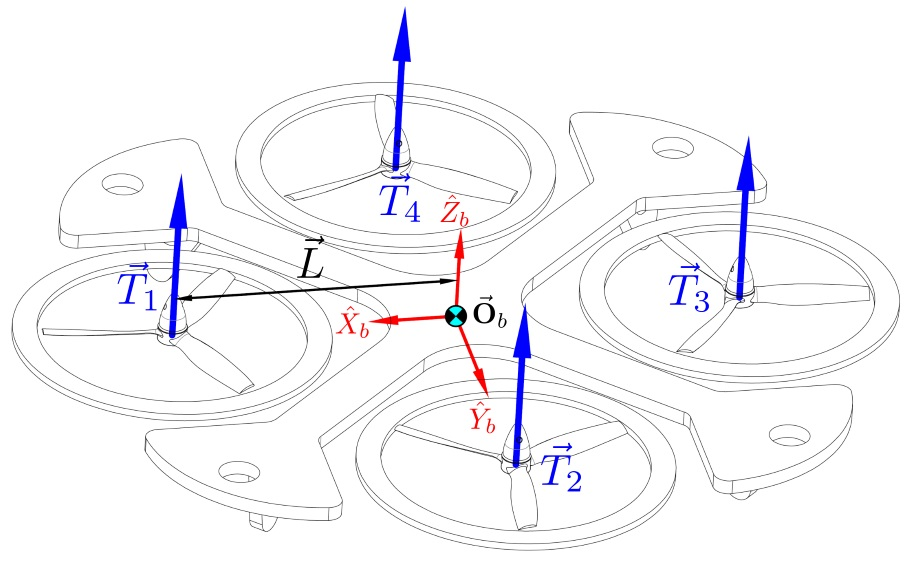
\includegraphics[width=0.8\textwidth]{figs/net-force}
\vspace{-10pt}
\caption{Generalized quadrotor net forces and torques}
\label{fig:net-force}
\vspace{-18pt}
\end{figure}
\par
Typically $\vec{F}_{\mu}$ is the net heave force acting on the center of motion $\vec{\mathbf{O}}_b$. The net heave is the sum of all thrust forces produced by rotating propellers, as some function of those rotational speeds; $\vec{T}(\Omega_i)$.
\begin{subequations}\label{eq:generalized-net-forces}
\begin{equation}
\vec{F}_{\mu} = \sum_{i=1}^4 \vec{T}(\Omega_i)\cdot\hat{Z}_b~~~~\in\mathcal{F}^b
\end{equation}
Similarly net torque $\vec{\tau}_{\mu}$ is the sum of all \emph{differential} torques produced from opposing propeller thrust vectors. Each torque arm $\vec{L}_{[1:4]}$ is the thrust's orthogonal displacement relative to the origin of \emph{motion}.
\begin{equation}
\vec{\tau}_{\mu} = \sum_{i=1}^4 \vec{L}_i \times \vec{T}(\Omega_i)\cdot\hat{Z}_b~~~~\in\mathcal{F}^{b}
\end{equation}
\end{subequations}
In Eq:\ref{eq:generalized-net-forces}, the thrust vector $\vec{T}(\Omega_i)$ is a function of the $i^{th}$ motor's rotational velocity $\Omega_i$, fixed in the $\hat{Z}_b$ direction. Each thrust vector could potentially be $\in\mathbb{R}^3$ such as the redirected vector from Eq:\ref{eq:motor-module-force-redirect}. All of the above equations are still applicable to any 6-DOF body; common simplifications applied to the system for quadrotor control are explored in App:\ref{app:equations.standard}. Aerodynamic components pertinent for thrust and torque generation relative to Eq:\ref{eq:generalized-net-forces} are now introduced; obviously the contextual focus is on quadrotor with dual-tilting axis actuators.
%====================================================
\section{Aerodynamics}
\label{sec:dynamics.aero}
%====================================================
Aerodynamic effects detailed here and subsequent nonlinear multibody responses in Sec:\ref{sec:dynamics.nonlinearities} both affect the generalized forces and torques acting on the body. The relationship between a propeller's rotational speed $\Omega_i$, in revolutions per second or [\emph{RPS}], and its perpendicular thrust vector $\vec{T}(\Omega_i)$ is more complicated than the quadratic simplification taken at static conditions which some papers assume (e.g \cite{x4flyer} etc\ldots). Produced thrust is mostly dependent on the incident air stream flowing through the propeller's rotational plane; typically being the body velocity's component normal to that propeller's plane. Fluid flowing \emph{tangentially} across the propeller's plane contributes toward in-plane aerodynamic drag and hence torque. 
\par
The combination of aerodynamic blade-element\cite{bem,forwarddescent} and fluid-dynamics momentum or \emph{disc actuator} theories equate an integral term generated across the propeller's length with the produced thrust or torque. A schedule of all aerodynamic effects encountered by a quadrotor's propellers is thoroughly detailed in both \cite{bladesforquadrotors} and \cite{nonlineardynamics}. The following is a review of pertinent aerodynamic theories; vortex ring state and parasitic drag effects are omitted as they will be approximately negligible given the aircraft's proposed flight envelope with low translational velocities.
%====================================================
\subsection{Propeller Torque and Thrust}
\label{subsec:dynamics.aero.bem}
%====================================================
\emph{\color{Gray} A possible situation which the prototype could encounter is where an upstream propeller provides the incident fluid flow to another downstream propeller. Such a situation presents a complicated fluid dynamics and vortex wake effect problem. Propeller overlapping effects are discussed in \cite{configurationpropulsion} but remain open to further research in the context of the aircraft considered here.}
\par
To expedite the system identification process some simplifications are made on the aerodynamics to construct an approximate model; specifically using coefficients in place of complete local chord and pitch based integrals. Such an assumption holds true given that twisted, fixed pitch propellers are used (Fig:\ref{fig:fixed-pitch}) and not variable pitch swash-plate actuated propellers (Fig:\ref{fig:variable-pitch}).
\begin{figure}[htbp]
\vspace{-8pt}
\centering
\begin{subfigure}{0.49\textwidth}
\centering
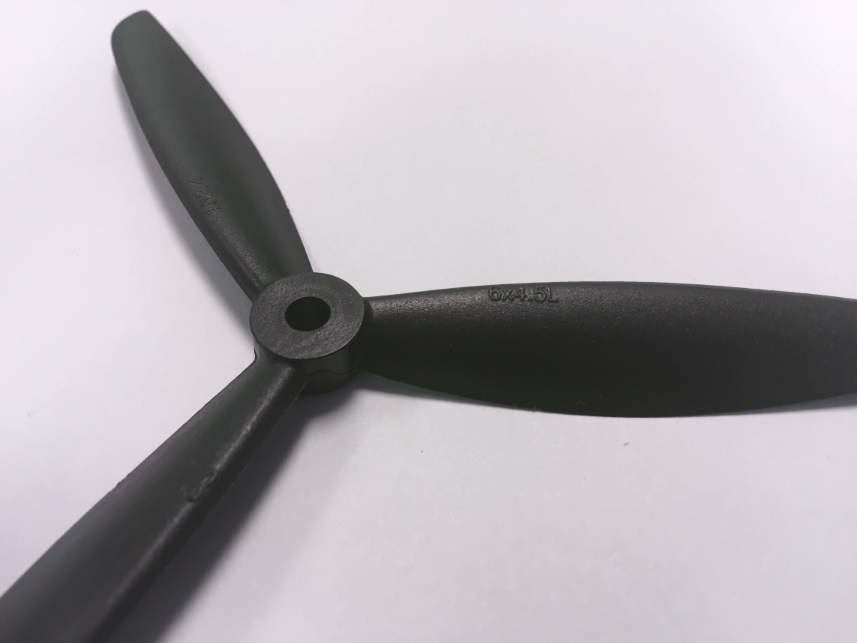
\includegraphics[width=0.8\textwidth]{figs/fixed-pitch}
\vspace{-4pt}
\caption{Twisted, fixed pitch}
\label{fig:fixed-pitch}
\end{subfigure}
\begin{subfigure}{0.49\textwidth}
\centering
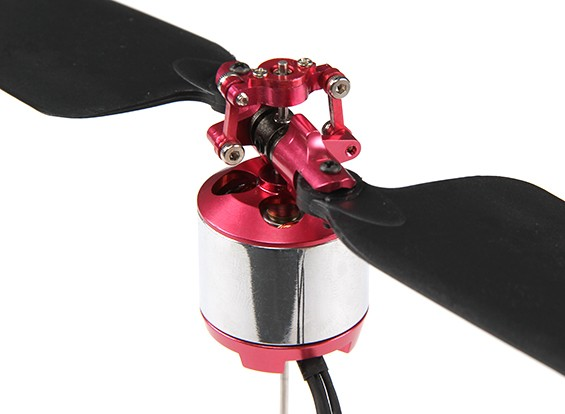
\includegraphics[width=0.8\textwidth]{figs/variable-pitch}
\vspace{-4pt}
\caption{Swash-plate variable pitch; \cite{variablepitch}}
\label{fig:variable-pitch}
\end{subfigure}
\vspace{-10pt}
\caption{Propeller types}
\label{fig:props}
\vspace{-18pt}
\end{figure}
\par
A propeller's profile applies a perpendicular scalar thrust force $T$ onto the fluid in which it rotates. To build the following theoretical explanation propellers are first considered in terms of momentum theory; only perpendicular fluid flow through the propeller's plane is regarded. That fluid stream (Fig:\ref{fig:bem-flow}) has an incident upstream velocity $v_\infty$ and a resultant slip velocity $v_s$ downstream relative to the rotational plane. The change of fluid flow as a result of the propeller's rotation can be given as:
\begin{equation}
v_s = \Delta v + v_\infty
\end{equation}
Where $\Delta v$ is the net change in fluid velocity caused by the propeller blade's rotating aerofoil profile. The propeller induces a velocity directly in front of its rotational plane $v_i$, such that the net fluid flow into the plane is $v_b=v_i+v_\infty$. That induced inflowing fluid velocity is different to the net velocity contribution of the propeller; $v_i\not=\Delta v$.
\par
\begin{figure}[htbp]
\centering
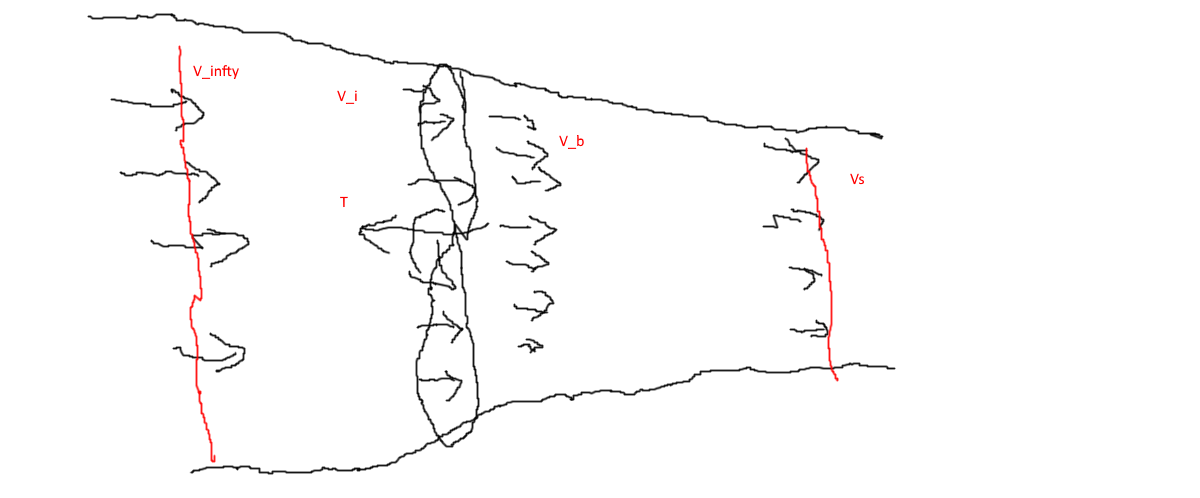
\includegraphics[width=0.85\textwidth]{figs/bem-flow}
\vspace{-12pt}
\caption{Disc Actuator Propeller Planar Flow}
\label{fig:bem-flow}
\vspace{-15pt}
\end{figure}
It is shown in \cite{bladesforquadrotors} that at static conditions, using Bernoulli's pressure theorem, the net fluid flow through the propeller's plane is:
\begin{equation}\label{eq:bernoulli}
v_b = \frac{1}{2} ( v_s - v_{\infty} ) = \frac{1}{2} \Delta v = \frac{1}{2} v_s \big|_{v_\infty=0}
\end{equation}
Stemming from classical disc actuator, or fluid \emph{momentum} theory \cite{fluidmomentum,propellers}, the scalar force $T(\Omega_i)$ acting on the fluid is calculated as a function of mass flow rate with respect to the change in fluid velocity or \emph{pressure differential}:
\begin{equation}\label{eq:prop-mass}
T=(A_b v_b)\Delta v = \rho \pi R_b^2v_b \Delta v = \rho \pi R_b^2(v_i+v_\infty)\Delta v = \frac{1}{2} \rho \pi R_b^2 \Delta v^2
\end{equation}
Where $R_b$ is the disc (propeller) radius in $\text{m}$ for the fluid stream under consideration, $A_b$ is the swept area of that propeller disc. The fluid density of that stream $\rho$ is typically $1.225~[\text{kg.m}^{-3}]$ at standard temperature and pressure (\emph{stp}). However, the desired form of thrust generated is as a function of propeller rotational velocity, $T(\Omega_i)$ in $[\text{RPS}]$, so Eq:\ref{eq:prop-mass} is not yet satisfactory. 
\par
Eq:\ref{eq:prop-mass} could be solved from the aerodynamic propulsive power expended; using $\Delta P=T\Delta v$. The relationship between rotational kinetic energy of a propeller and its transferred propulsive power is difficult to quantify, compound parasitic losses deteriorate the efficiency of the propeller and motor. Furthermore, the fluid velocity through the propeller's plane is not purely normal but is in fact a vector. 
\par
Fluid flow induced by the propeller's rotation $v_i$ directly in front of its plane of rotation has both axial and tangential induced components, termed $a$ and $a'$ respectively. Induced fluid velocity components are abstracted to induction factors which are dependent on the incident fluid velocity entering the propeller's plane of rotation:
\begin{subequations}\label{eq:induction-factors}
\vspace{-5pt}
\begin{equation}\label{eq:induction-axial}
v_i=a v_\infty~~\text{in the axial direction}
\end{equation}
\vspace{-16pt}
\begin{equation}\label{eq:induction-tangential}
v_\theta=a' \Omega_i R_b~~\text{in the tangential direction}
\end{equation}
\end{subequations}
Using the induction factors to rewrite the fluid's through velocity $v_b$ and its slip stream velocity $v_\infty$:
\begin{subequations}
\vspace{-5pt}
\begin{equation}
v_b=(1+a)v_\infty
\end{equation}
\vspace{-18pt}
\begin{equation}
v_s=(1+2a)v_\infty
\end{equation}
\end{subequations}
A consequence of the tangential fluid flow is that an angular momentum flow rate exists across the propeller plane. This produces a fluid-momentum torque opposing the rotational motion about the propeller's axis, analogous but perpendicular to Eq:\ref{eq:prop-mass}:
\begin{equation}\label{eq:prop-moment}
H=\rho\pi R_b^3 (v_\theta-v_\infty) v_b 
\end{equation}
\par
Together, Eq:\ref{eq:prop-mass} and Eq:\ref{eq:prop-moment} comprise propeller momentum theory but cannot be solved on their own. Blade-element theory analyses incremental aerofoil sections of width $dr$ of the propeller profile  at some radius $r$, the sectional view of which is illustrated in Fig:\ref{fig:bem-profile}. Each aerofoil element has a net local fluid velocity $\vec{U}$ across its profile, calculated as:
\begin{equation}
\vec{U}=\sqrt{(v_\infty+v_i)^2+(v_\Omega+v_\theta)^2}
\end{equation}
Where each profile has a chord length $c$ and an inclination (or \emph{pitch}) $\theta$ of the aerofoil \emph{zero-lift line} relative to the horizontal. Local fluid velocities incident to the propeller profile (Fig:\ref{fig:bem-profile}) make their own angle of attack $\phi$ such that a true effective angle of attack $\alpha_{eff}$ is encountered:
\begin{equation}
\phi=\theta-\alpha_{eff}
\end{equation}
That local angle of attack varies with the incident fluid flow magnitude $v_\infty$ and the induced axial velocity $v_i$. The trigonometric ratio between the two is given as:
\begin{equation}
\phi=tan^{-1}\bigg(\frac{v_\infty+v_i}{v_\Omega+v_\theta}\bigg)=tan^{-1}\bigg(\frac{v_\infty(1+a)}{\Omega r(1+a')}\bigg)
\end{equation}
\par
\begin{figure}[hbtp]
\vspace{-15pt}
\centering
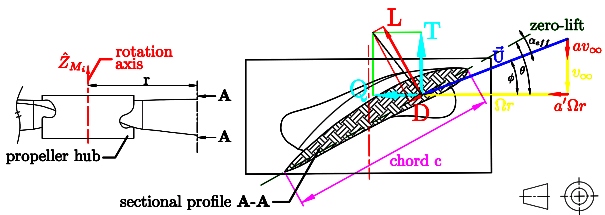
\includegraphics[width=\textwidth]{figs/bem-profile}
\caption{Blade element profile at radius r}
\label{fig:bem-profile}
\end{figure}
In-plane fluid flow $\vec{U}(r,\phi)$, for an element at radius $r$ with a local angle of attack $\phi$, then contributes towards elemental lift and drag forces as a function of aerofoil's dimensionless lift, $C_L$, and drag, $C_D$, coefficients. Those coefficients are determined by the aerofoil's characteristics, but would be constant across the length of a variable pitch, hinged and untwisted flat propeller (Fig:\ref{fig:variable-pitch}).
\begin{subequations}
\begin{equation}
\Delta L=\frac{1}{2}\rho \vec{U}(r,\phi)^2 c C_L
\end{equation}
\vspace{-10pt}
\begin{equation}
\Delta D=\frac{1}{2}\rho \vec{U}(r,\phi)^2 c C_D
\end{equation}
\end{subequations}
With air density $\rho$ again at \emph{stp}. Lift and drag forces, when taken parallel and perpendicular to the plane of rotation, are thrust $T$ and torque $F_H$ forces (Fig:\ref{fig:bem-profile}). The in-plane force applies an aerodynamic torque $H$ at the propellers hub because the force $F_H$ acts at a radius $r$, \cite{starmac}.
\begin{subequations}
\begin{equation}\label{eq:element-thrust}
dT=\frac{1}{2}\rho\vec{U}(r,\phi)^2c\big(C_L cos(\theta)+C_D sin(\theta)\big).dr
\end{equation}
\vspace{-5pt}
\begin{equation}\label{eq:element-drag}
dF_H=\frac{1}{2}\rho\vec{U}(r,\phi)^2c\big(C_L sin(\theta)+C_D cos(\theta)\big).dr
\end{equation}
\vspace{-5pt}
\begin{equation}\label{eq:element-torque}
\therefore dH = \frac{1}{2}\rho\vec{U}(r,\phi)^2c\big(C_L sin(\theta)+C_D cos(\theta)\big)r.dr
\end{equation}
\vspace{-10pt}
\begin{equation}\label{eq:element-power}
\therefore dP = \Omega r dF_H .dr
\end{equation}
\end{subequations}
\par
Rotational power expended is a product of angular velocity and the opposing in-plane torque; Eq:\ref{eq:element-power}. Power is mostly used instead of torque or drag terms in Eq:\ref{eq:element-torque} or Eq:\ref{eq:element-drag} respectively. Calculating forces and power terms as per momentum theory for each element, in terms of axial and tangential induction factors:
\begin{subequations}\label{eq:moment-thrust-element}
\begin{equation}
dT=\rho 4 \pi r^2 v_\infty(1+a)a.dr
\end{equation}
\vspace{-16pt}
\begin{equation}
dP=\rho 4 \pi r^2 v_\infty(1+a)\Omega r (1+a').dr
\end{equation}
\end{subequations}
Equating momentum and element terms produces the blade-element momentum equation(s) for aerodynamic thrust and power from a propeller. Following a few assumptions; most importantly that the lift coefficient $C_L$ is a linear function of the effective angle of attack $\alpha_{eff}$, typically characterized as:
\begin{equation}
C_L=a_L(\theta-\phi)
\end{equation}
Firstly the lift coefficient curve gradient $a_L$ is shown in \cite{aerodynamicsforengineering} for an ideally twisted blade, like the fixed pitch propellers under consideration, to be $2\pi$. An ideal lift coefficient is then a function:
\begin{equation}\label{eq:lift-curve-gradient}
C_L=2\pi(\theta-\phi)
\end{equation}
Secondly, assuming tangentially induced velocities $v_\theta$ are small when compared to the propeller's translational speed at radius $r$, $v(\Omega_i)=\Omega_i r$. The tangential induction factor $a'$ is then the ratio:
\begin{equation}
a'=\frac{v_\theta}{\Omega_i r}<<1
\end{equation}
Small angle approximations then apply to Eq:\ref{eq:element-thrust}-\ref{eq:element-torque}; $cos(\phi+\alpha_{eff})\approx 1$ and $sin(\phi+\alpha_{eff})\approx \phi+\alpha_{eff}$. Similarly net inflow and axial velocities are $(v_\infty + v_i)<<\Omega_i r$, the following integrals are then found:
\begin{subequations}
\begin{equation}\label{eq:bem-thrust}
T(\Omega_i)=\int_{r=0}^R \frac{1}{2} a_L b c \rho (\Omega_i r)^2 \bigg[\theta-\frac{v_\infty+v_i}{\Omega_i r}\bigg].dr
\end{equation}
\begin{equation}\label{eq:bem-power}
P(\Omega_i)=\int_{r=0}^R \frac{1}{2}a_L b c \rho (\Omega_i r)^3\bigg[\big(\theta-\frac{v_\infty+v_i}{\Omega_i r}\big)\big(\frac{v_\infty+v_i}{\Omega_i r}\big) + C_d\bigg].dr
\end{equation}
\end{subequations}
Where $b$ is the number of blades the propeller has. In practice knowing exact pitch and chord values as a function of $r/R$ is difficult and calculating integrals at each process step is cumbersome. Both Eq:\ref{eq:bem-thrust} and Eq:\ref{eq:bem-power} can be solved by equating element and momentum terms, a full solution of which is given in App:\ref{app:equations.bem}. Often dimensionless thrust and power coefficients are defined across the entire blade's length:
\begin{subequations}\label{eq:coefficients}
\begin{equation}\label{eq:thrust-coefficient}
C_T(J)\triangleq\frac{T}{\rho \Omega_i\hspace{-2pt}^2 D^4}
\end{equation}
\vspace{-6pt}
\begin{equation}\label{eq:power-coefficient}
C_P(J)\triangleq\frac{P}{\rho \Omega_i\hspace{-2pt}^3 D^5}
\end{equation}
\end{subequations}
Where the propeller's diameter is $D$ in $[\text{m}]$, then $\Omega_i$ is the propeller's rotational speed in \emph{revolutions per second} [\emph{RPS}] and different from other inertial equations like Eq:\ref{eq:angular-rot}, with units $[\text{rad.s}^{-1}]$. For fixed pitch propellers the thrust and power coefficients are easily determined and remain consistent. Both Eq:\ref{eq:thrust-coefficient} and Eq:\ref{eq:power-coefficient} vary as a function of the dimensionless \emph{advance ratio} $J$.
\begin{equation}\label{eq:advance}
J\triangleq\frac{v_\infty}{\Omega_i R}
\end{equation}
Typically the net upstream velocity $v_\infty$ in Eq:\ref{eq:advance} is simply the perpendicular component (projected onto the plane's normal vector $\hat{n}$, shown later in Eq:\ref{eq:normal-fluid}) of the vehicle's translational velocity in the body frame; $\vec{v}_b\perp\hat{n}$. For the case of a zero advance ratio $J=0$, the conditions are regarded as static. Static thrust and power coefficients are nominal in their values.
\par
Propeller databases like \cite{UIUC} provide comprehensive coefficient values for a range of small and medium diameter propeller types at different advance ratios. Included in the database are blade profiles, pitch and chord lengths; all the results are outcomes of the investigation \cite{lowreynolds}. 
\par
The introduction of those coefficients drastically reduces thrust estimation complexity. For a typical $6\times 4.5$ inch propeller the following coefficients were linearly interpolated from similar pitched database results in \cite{UIUC} to match subsequent physical test values. Static thrust and power coefficients determined from tests subsequently in Fig:\ref{fig:thrust-plot} and Fig:\ref{fig:torque-plot} are respectively:
\begin{subequations}
\begin{equation}
{\color{blue}C_{T0}}=0.191
\end{equation}
\vspace{-15pt}
\begin{equation}
{\color{red}C_{P0}}=0.0877
\end{equation}
\end{subequations}
Fig:\ref{fig:coeffs-plot} plots interpolated coefficients for thrust {$\color{Blue}C_{T}$} and power {$\color{Red}C_{P}$} as a function of the advance ratio $J$. As the incident upstream fluid velocity $v_\infty$ increases, the thrust coefficient decreases. So too does the power coefficient and hence the aerodynamic torque. The thrust and power coefficients can be assumed constant for low advance ratios, or in the case considered here, translational velocities.
\begin{figure}[htpb]
\centering
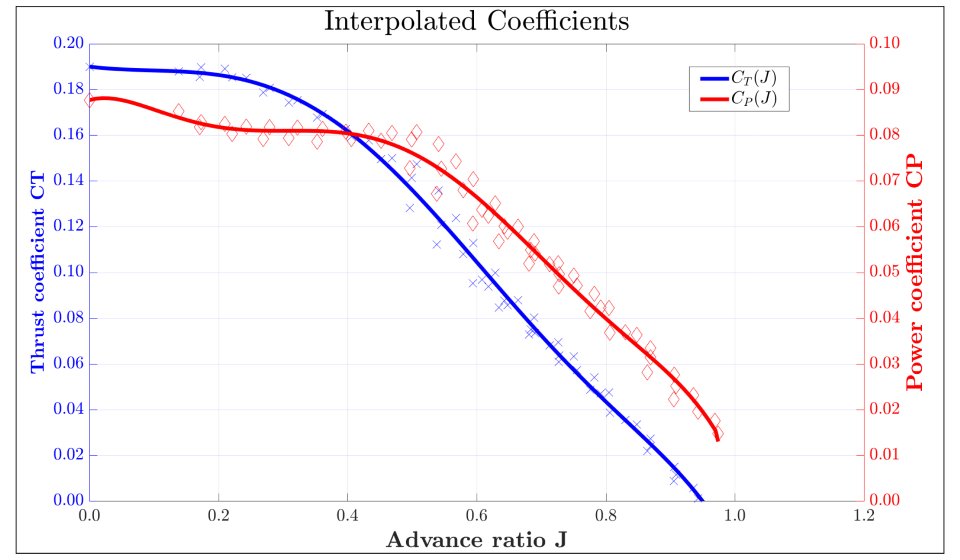
\includegraphics[width=0.74\textwidth]{graphs/coeffs-plot}
\vspace{-4pt}
\caption{Thrust and power coefficients}
\vspace{-18pt}
\label{fig:coeffs-plot}
\end{figure}
\par
Static thrust and torque tests were respectively performed on test rigs in Fig:\ref{fig:thrust-rig} and Fig:\ref{fig:torque-rig}. Measured values for each test are plotted; {\color{Red}$T(\Omega)$} in Fig:\ref{fig:thrust-plot} for thrust and {\color{Red}$H(\Omega)$} in Fig:\ref{fig:torque-plot} for torque. The physically tested values are fitted with quadratic trend-lines and plotted against static coefficient estimates using Eq:\ref{eq:thrust-coefficient} for thrust {\color{LimeGreen}$\hat{T}C_t(\Omega)$} and Eq:\ref{eq:power-coefficient} for calculated torque {\color{LimeGreen}$\hat{H}C_p(\Omega)$}. Results from Fig:\ref{fig:coeffs-plot} are used as a lookup table and values from Eq:\ref{eq:coefficients} are calculated, induced propeller thrust and torques can be accurately modelled quadratically, power is cubic with respect to rotational velocity. 
\begin{figure}[htbp]
\centering
\begin{subfigure}{0.49\textwidth}
\centering
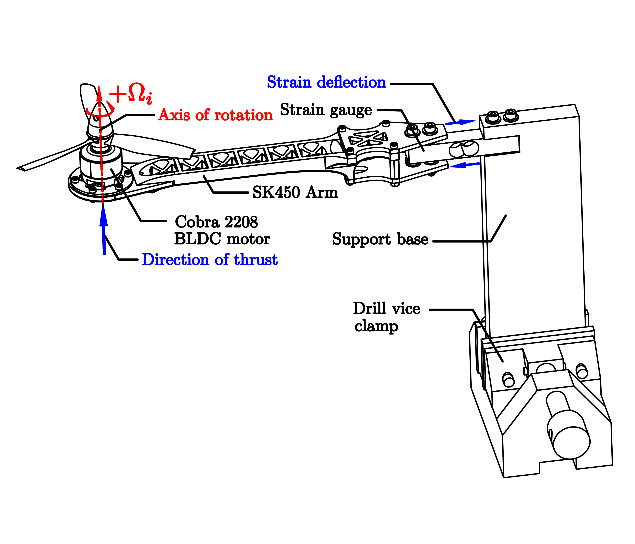
\includegraphics[width=\textwidth]{figs/thrust-rig}
\vspace{-10pt}
\caption{Propeller thrust test rig}
\label{fig:thrust-rig}
\end{subfigure}
\begin{subfigure}{0.49\textwidth}
\centering
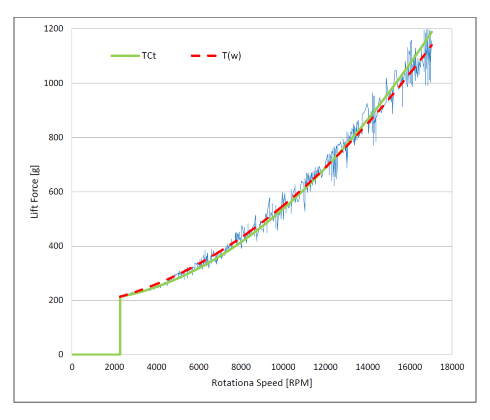
\includegraphics[width=\textwidth]{graphs/thrust-plot}
\vspace{-10pt}
\caption{Static lift force results}
\label{fig:thrust-plot}
\end{subfigure}
\vspace{-4pt}
\caption{Propeller thrust tests}
\label{fig:thrusts}
\end{figure}
\par
\begin{figure}[hbtp]
\begin{subfigure}{0.5\textwidth}
\centering
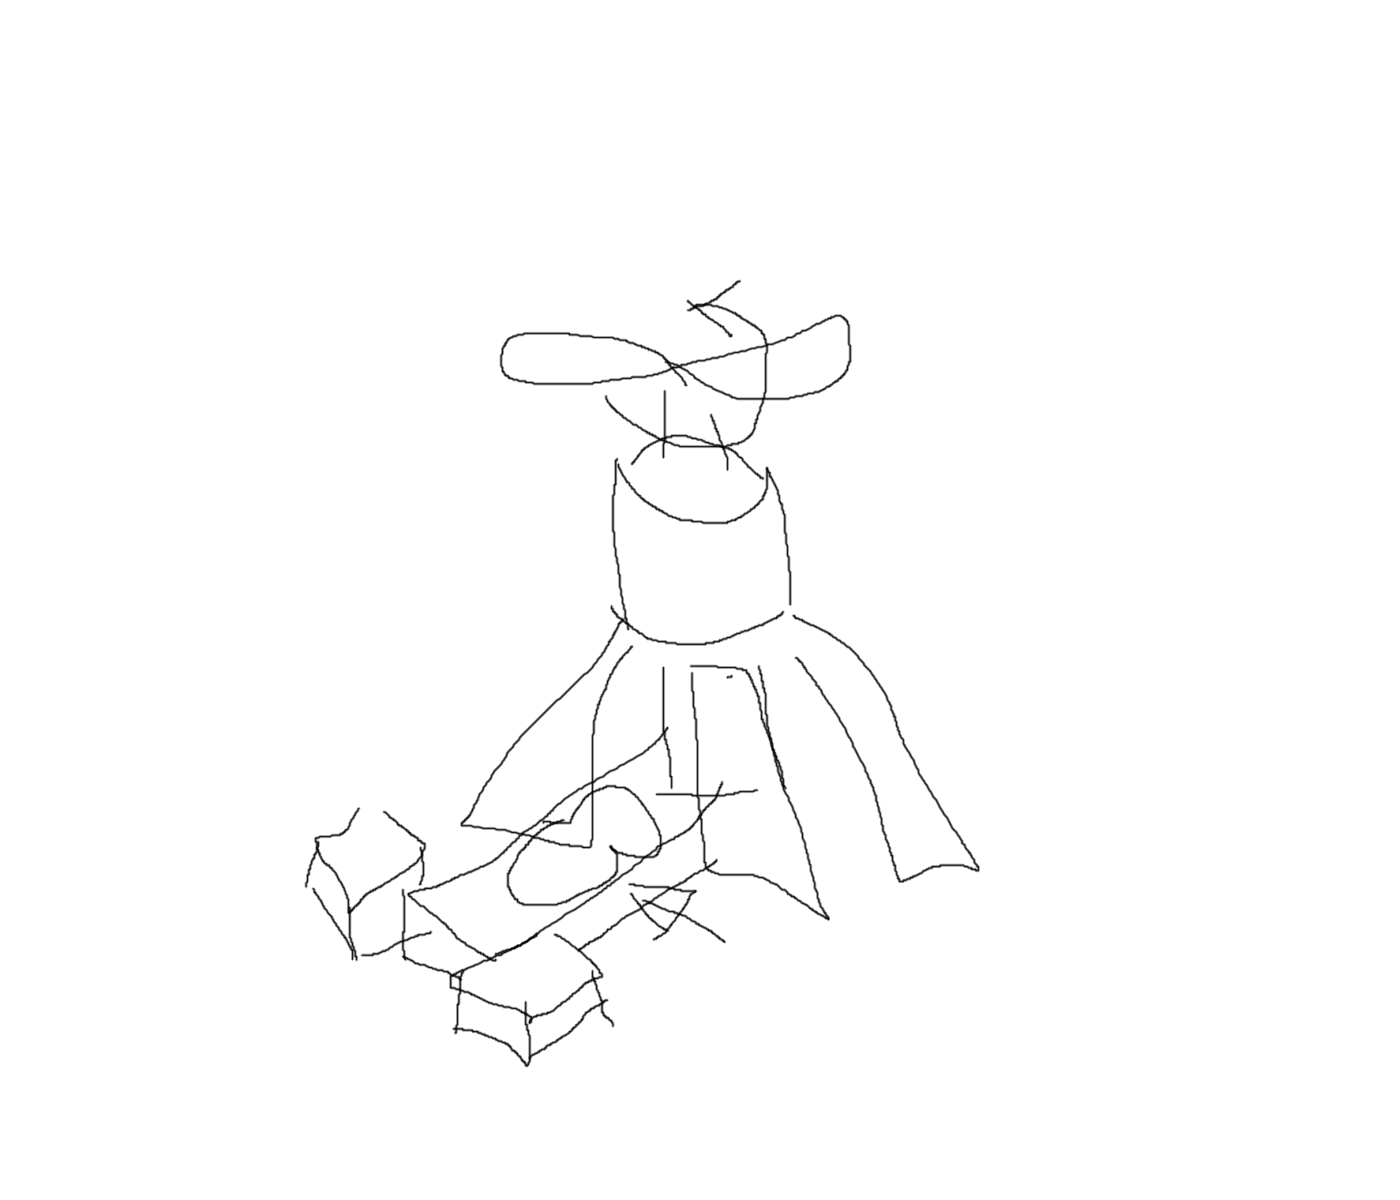
\includegraphics[width=\textwidth]{figs/torque-rig}
\vspace{-10pt}
\caption{Aerodynamic drag torque test rig}
\label{fig:torque-rig}
\end{subfigure}
\begin{subfigure}{0.5\textwidth}
\centering
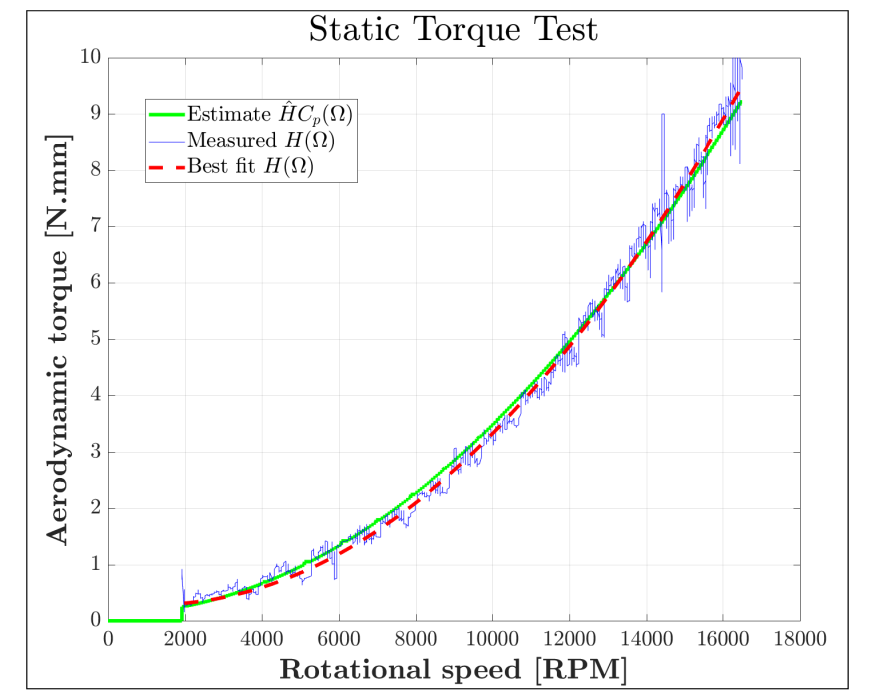
\includegraphics[width=\textwidth]{graphs/torque-plot}
\vspace{-10pt}
\caption{Torque plot}
\label{fig:torque-plot}
\end{subfigure}
\vspace{-4pt}
\caption{Static induced torque results}
\label{fig:torques}
\vspace{-16pt}
\end{figure}
\par
Advance ratios, Eq:\ref{eq:advance}, or rather the propeller incident fluid flows are dependent on the vehicle's net translational and angular velocity. Such that the fluid velocity's normal component to the propeller plane is given by:
\begin{equation}\label{eq:normal-fluid}
v_\infty = (\vec{v}_b\hspace{-1pt}' + \vec{L}_{arm}\times \vec{\omega}_b\hspace{-1pt}')\cdot \hat{n}(\lambda_i,\alpha_i)~~~~\in\mathcal{F}^{M_i}
\end{equation}
Where $\vec{v}_b\hspace{-1pt}'$ in $[\text{m.s}^{-1}]$ is the body's translational velocity and $\vec{\omega}_b\hspace{-1pt}'$ in $[\text{rad.s}^{-1}]$ is the body's angular velocity, both transformed to the propeller's frame, $\in\mathcal{F}^{M_i}$. Furthermore $\hat{n}(\lambda_i,\alpha_i)$ is the unit vector normal to the propeller's rotational plane, relative to the body velocity. Then $J$ is calculated from Eq:\ref{eq:advance}.
\par
{\color{Gray}\emph{It is worth reiterating that the above static coefficients are indeed calculated from physical static tests. However advance ratio coefficient dependencies are linearly interpolated from the closest available matching data (APC Thin-Electric 8X6 propellers) cited from \cite{UIUC}}.}
\par
Clockwise and anti-clockwise propellers and rotations were used for both thrust and torque tests. Despite both test rigs  (Fig:\ref{fig:thrust-rig} and Fig:\ref{fig:torque-rig} respectively) having been designed to specifically isolate each response, results from opposing directional tests were averaged in the hopes that stray opposing effects would cancel. Both clockwise and anti-clockwise rotational testing  results for thrust and torque measurements are included in App:\ref{app:thrust-torque}
\par
{\color{Gray}\emph{Discrepancies which exist between the model or coefficient values derived can be accounted for with lumped uncertainty disturbance terms. Model uncertainty compensation can easily be incorporated into adaptive backstepping or $H_\infty$ control algorithms. The deviation of the modelled thrust or torques from their true values would be simple to incorporate into a plant dependent Lyapunov candidate function; Sec:\ref{subsubsec:control.attitude.nonlinear.adaptivebackstep}.}}
%====================================================
\subsection{Hinged Propeller Conning \& Flapping}
\label{subsec:dynamics.aero.flap}
%====================================================
Aerodynamics which adversly affect a propeller's performance have all been well documented in their own right; mostly in the context of helicopter aerodynamic and propeller fields\cite{basichelicopter,bramwell}. Typically such effects are more pronounced when observing hinged variable pitch propellers (Fig:\ref{fig:variable-pitch}), fixed pitch propellers with small radii have a diminished effect. Moreover, low translational velocities suppress such responses but they're worth mentioning.
\par
Conning and flapping are the two most significant aerodynamic effects encountered by a propeller. Other phenomenon like cyclic vortex ring states are deemed to be inapplicable here and fall outside the scope of the investigation. 
\par
In translational flight, for a propeller without shrouding or a ducting, each blade encounters varying incident fluid flow throughout its cycle. The advancing blade relative to the body's translational direction encounters a greater fluid flow than the retreating blade, constructive and destructive interference from the body's translational velocity adds to local fluid flows. The effective local angle of attack, sectional Fig:\ref{fig:bem-profile}, for advancing and retreating propeller blades are then asymmetrical. Unbalanced angles of attack produce a dissymmetry of lift across the propeller blade's surface.
\par
\begin{figure}[htbp]
\centering
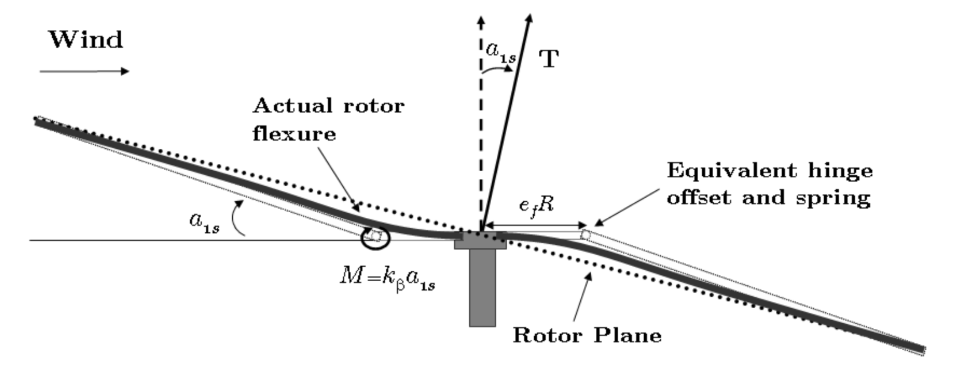
\includegraphics[width=\textwidth]{figs/prop-flap}
\caption{Propeller blade flapping; from \cite{starmac}}
\label{fig:prop-flap}
\end{figure}
\par
Throughout each rotation the blade is forced up and down as it cycles through a varying fluid velocity field, applying a torque moment about the propeller's hub. That torque's magnitude is a function of the body's net translational velocity and the propeller material's stiffness and hence its susceptibility to deflection. The flapping pitches the effective propeller plane or \emph{tip-path plane}, and hence the thrust vector line, away from its principle axis; shown in Fig:\ref{fig:prop-flap}.
\par
The propeller's resultant thrust vector is pitched away from its perpendicular normal by some deflection angle, $\alpha_{1s}$ in Fig:\ref{fig:prop-flap}, toward the direction of translational movement or wind disturbance. Propeller flapping is diminished at low translational velocities with small wind disturbances relative to propeller rotational speed. As such flapping is not applicable to the feasible flight envelope envisaged for the prototype here.
\par
\begin{figure}[hbtp]
\centering
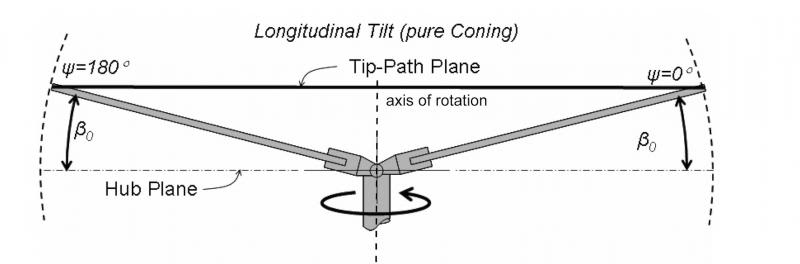
\includegraphics[width=0.95\textwidth]{figs/prop-coning}
\caption{Propeller coning}
\label{fig:prop-coning}
\end{figure}
Coning is another form of propeller deflection, illustrated in Fig:\ref{fig:prop-coning}, which again is dependent on the blade material's stiffness. Coning causes both advancing and retreating propeller blades to both deflect upward. Distributed loading on the propeller surface from supporting a body's weight causes the upward deflection. The coning reduces the effective propeller disc's radius, adversely affecting thrust produced, Eq:\ref{eq:bem-thrust}. Increased loading accentuates the coning angle experienced by the propellers and as such reduces the tip-path plane.
\par
Both aerodynamic propeller deflections can be quantified numerically. Their derivation and resultant equations are cumbersome however. In practice both effects on the produced prototype are not significant enough to affect the derived plant model. The frame could potentially be affected in more adverse ways given certain flight conditions with higher translational velocities or incident wind and fluid flow disturbances\ldots
%====================================================
\subsection{Drag}
\label{subsec:dynamics.aero.drag}
%====================================================
For any solid body with some non-zero relative translational velocity through a fluid, that fluid has a second order damping response opposing the body's movement. Net drag $\vec{D}_{net}$ is locally dependent on individual component cross-sections, for a vehicle's velocity $\vec{v}_b=[u~v~w]^T$ in $\mathcal{F}^b$, the drag force is:
\begin{equation}\label{eq:distrubance}
\vec{D}_{net}(\vec{v}_b)=\begin{bmatrix}
D_{ii} & D_{ij} & D_{ik}\\
D_{ji} & D_{jj} & D_{jk}\\
D_{ki} & D_{kj} & C_{kk}
\end{bmatrix}
\begin{bmatrix}
u\\
v\\
w
\end{bmatrix}^2
~~~~\in\mathcal{F}^b
\end{equation}
Each drag coefficient's subscript; $\hat{\imath},\hat{\jmath}$ and $\hat{k}$ is dependent on the body's directional cross-section area for each $\hat{X}_b,\hat{Y}_b,\hat{Z}_b$ axis respectively. Given a well designed and symmetrical frame, it can be assumed the off-diagonal elements are of little or no consequence and as such the drag equation can be simplified to the diagonal:
\begin{equation}
\vec{D}_{net}(\vec{v}_b)\approx diag\big(D_{ii},~D_{jj},~D_{kk}\big)\vec{v}_b^{\hspace{2pt}2}~~~~\in\mathcal{F}^b
\end{equation}
Due to the second order degree of translational velocity on the drag force; such terms can be relegated to a lumped disturbance terms to be compensated for in the control loop, Sec:\ref{subsubsec:control.attitude.nonlinear.adaptivebackstep}. The time scale separation between velocity and wind drag effects within the control loop accommodates such an assumption. Analogous rotational drag-like effects opposing angular rates exist but, for the intents and purposes of most practical flight envelopes, can be disregarded. 
\par
In simulation; if the plant has sufficient disturbance rejection then the drag term in Eq:\ref{eq:distrubance} would be easily accounted for in an adaptive backstepping algorithm. Drag, much like wind turbulence, is shown later in Sec:\ref{sec:simulation.disturbance} to be not consequential enough to be destabilizing. Furthermore it is possible to physically test for the drag coefficients to attain a higher certainty model but, given the flight conditions proposed for this research, such effects will be small if not negligible. As such those tests are outside the scope of investigation here.
%====================================================
\section{Quaternion Attitude}
%====================================================
\subsection{Rotation Matrix Singularity}\label{subsec:dynamics.rigidbody.singularity}
%====================================================
The singularity inherent to Euler angle parametrization is often mentioned but far less common is the mathematical demonstration of how that singularity manifests itself.  In general, a singularity occurs for some matrix $A$ in $\vec{y}=A\vec{x}$ when the matrix has a zero determinate; losing rank and hence differentiability of $\vec{y}$ in terms of $\vec{x}$. The combined rotation matrix from the inertial frame $\mathcal{F}^{I}$ to the body frame $\mathcal{F}^{b}$ is the singular component of an Euler parametrized sequence. 
\par
Considering the case of a rotational 3-axis gimbal system, illustrated in Fig:\ref{fig:gimbal}, which mimics the sequential nature of the Euler set. When the intermediary sequenced rotational angle is at $\pi/2$ rad, the remaining two axes become co-linear, Fig:\ref{fig:gimbal-lock}. In a ZYX rotation sequence, as adopted in this work, the singularity occurs from the rolling angle $\theta$ about the $\hat{Y}$ axis. Both the pitch $\phi$ and yaw $\psi$ rotations will subsequently have the same rotational effect. Such a situation results in as a loss of a degree of freedom.
\newpage
\begin{figure}[htbp]
\begin{subfigure}{0.5\textwidth}
\centering
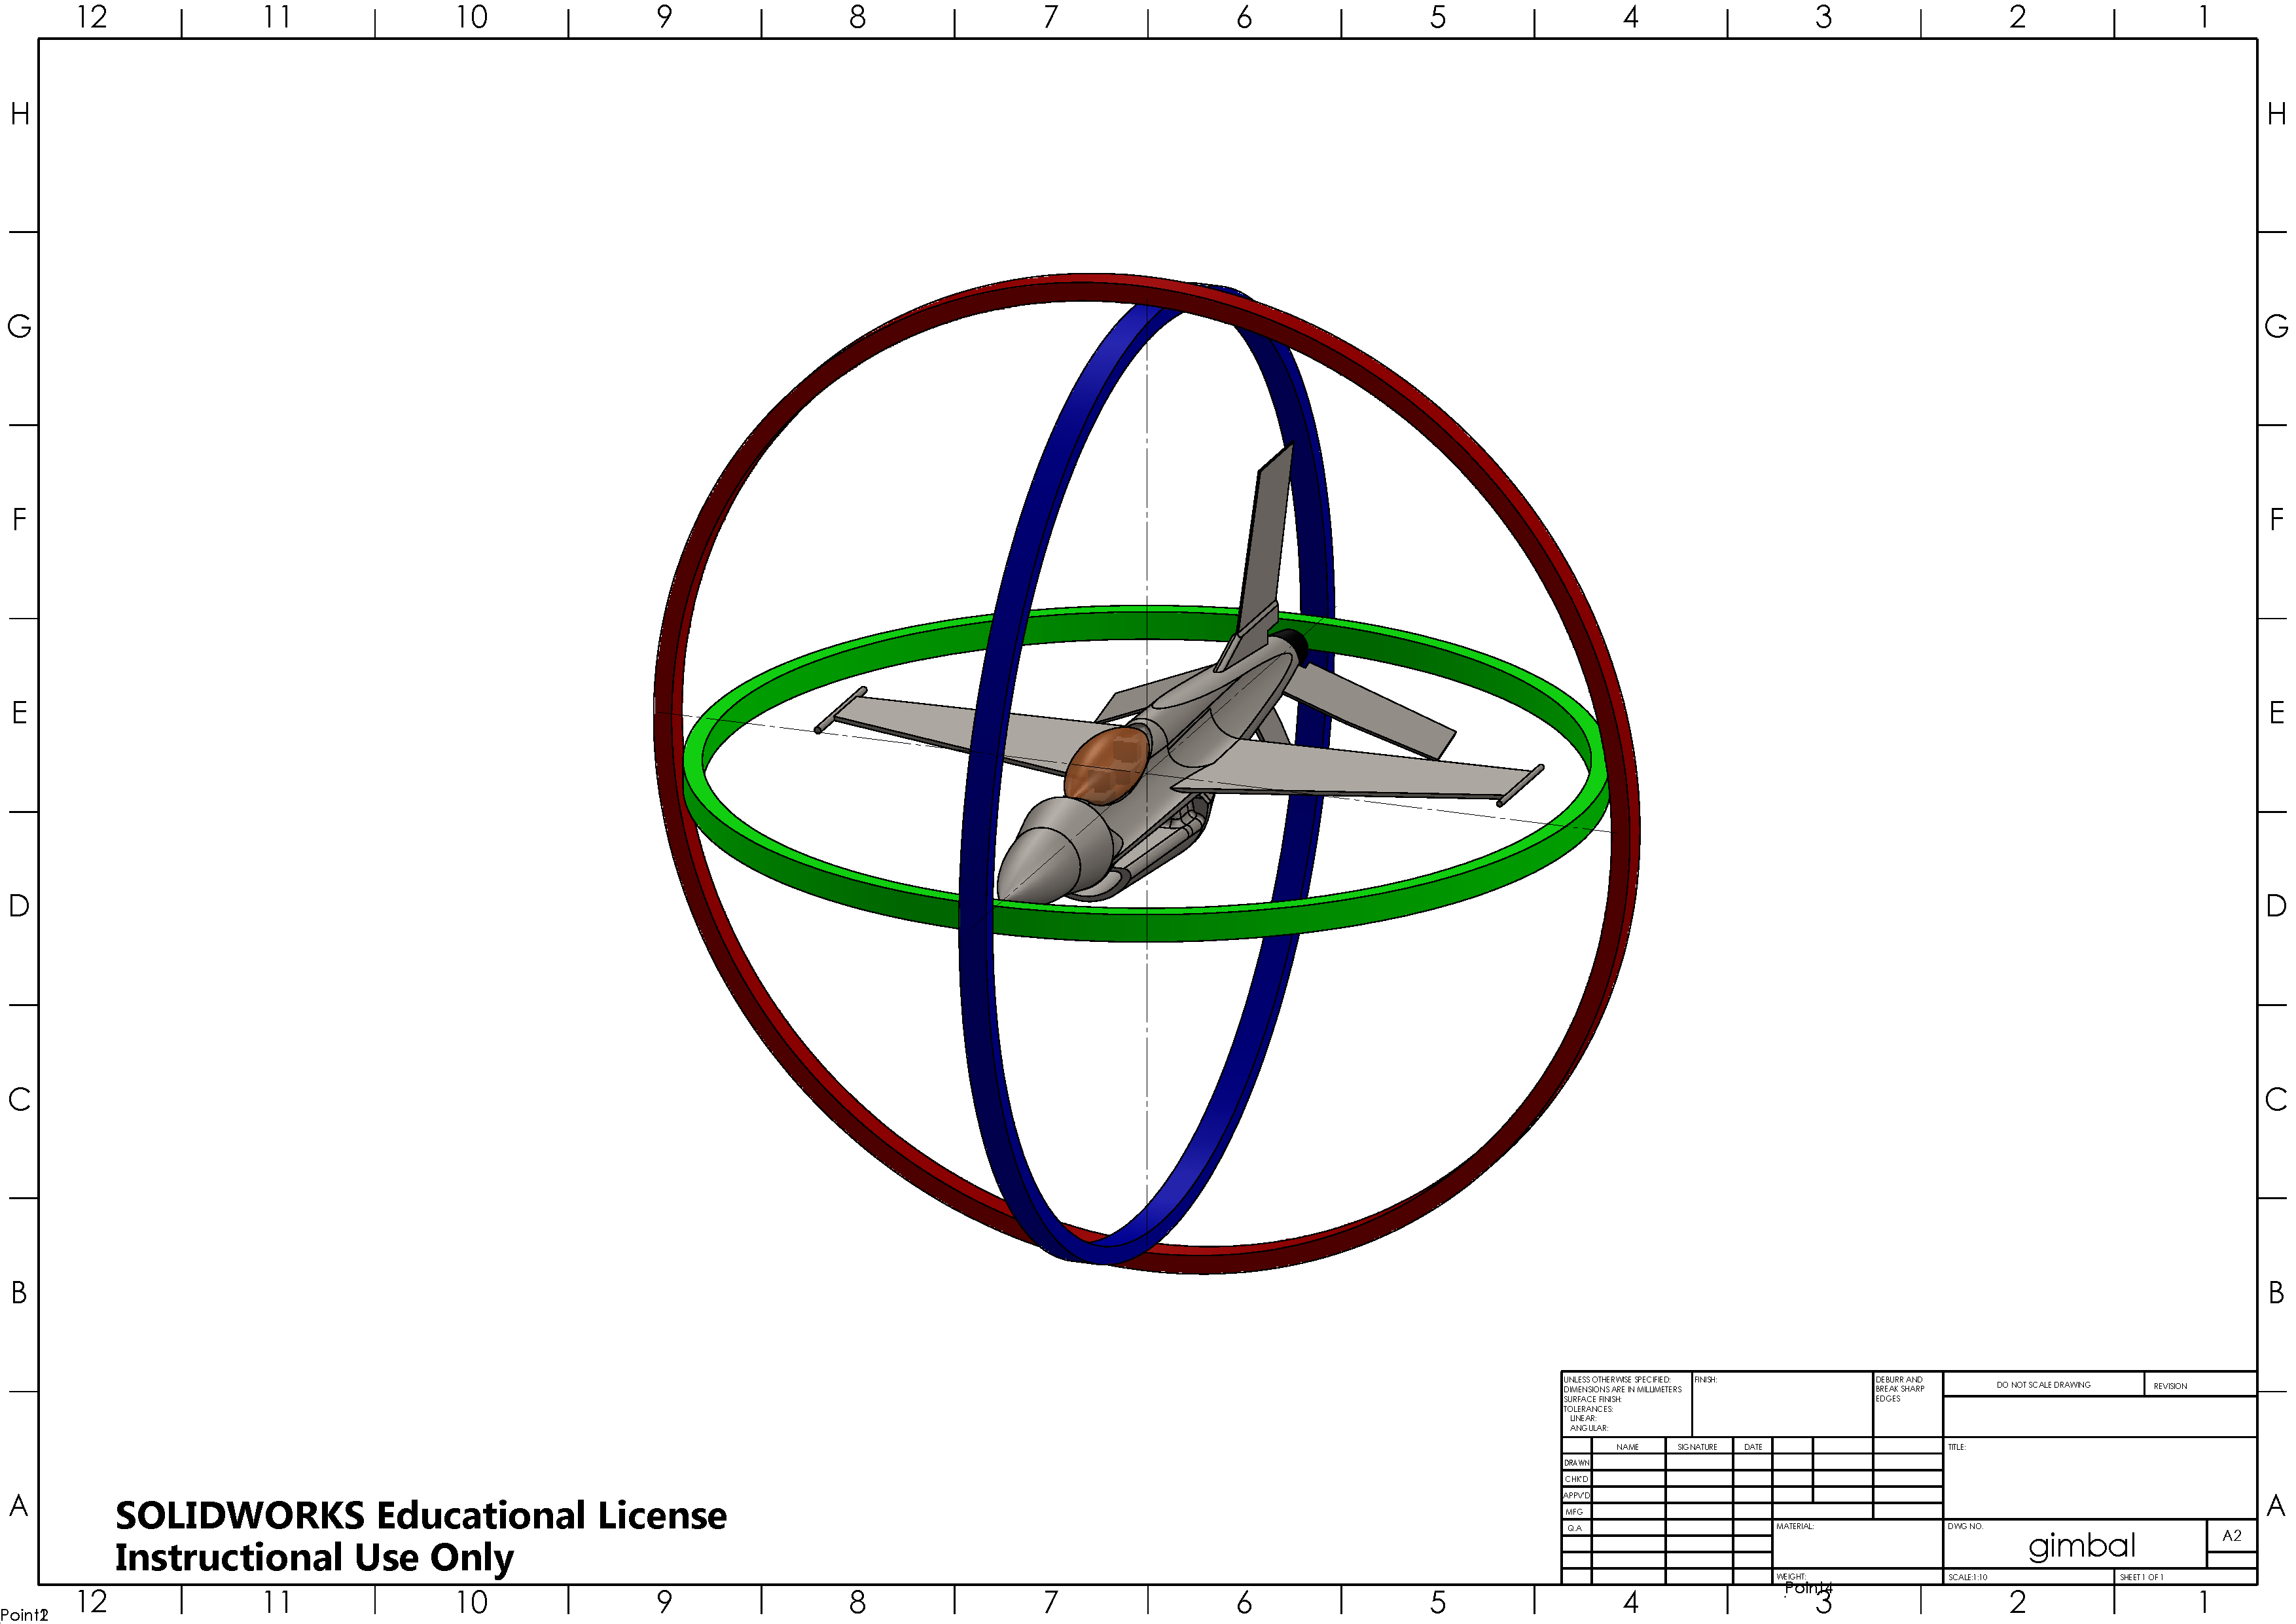
\includegraphics[clip, trim=16.5cm 8.5cm 16.5cm 6.7cm, width=0.93\textwidth]{pdfpages/gimbal}
\caption{3-Axis gimbal}
\label{fig:gimbal}
\end{subfigure}
\begin{subfigure}{0.5\textwidth}
\centering
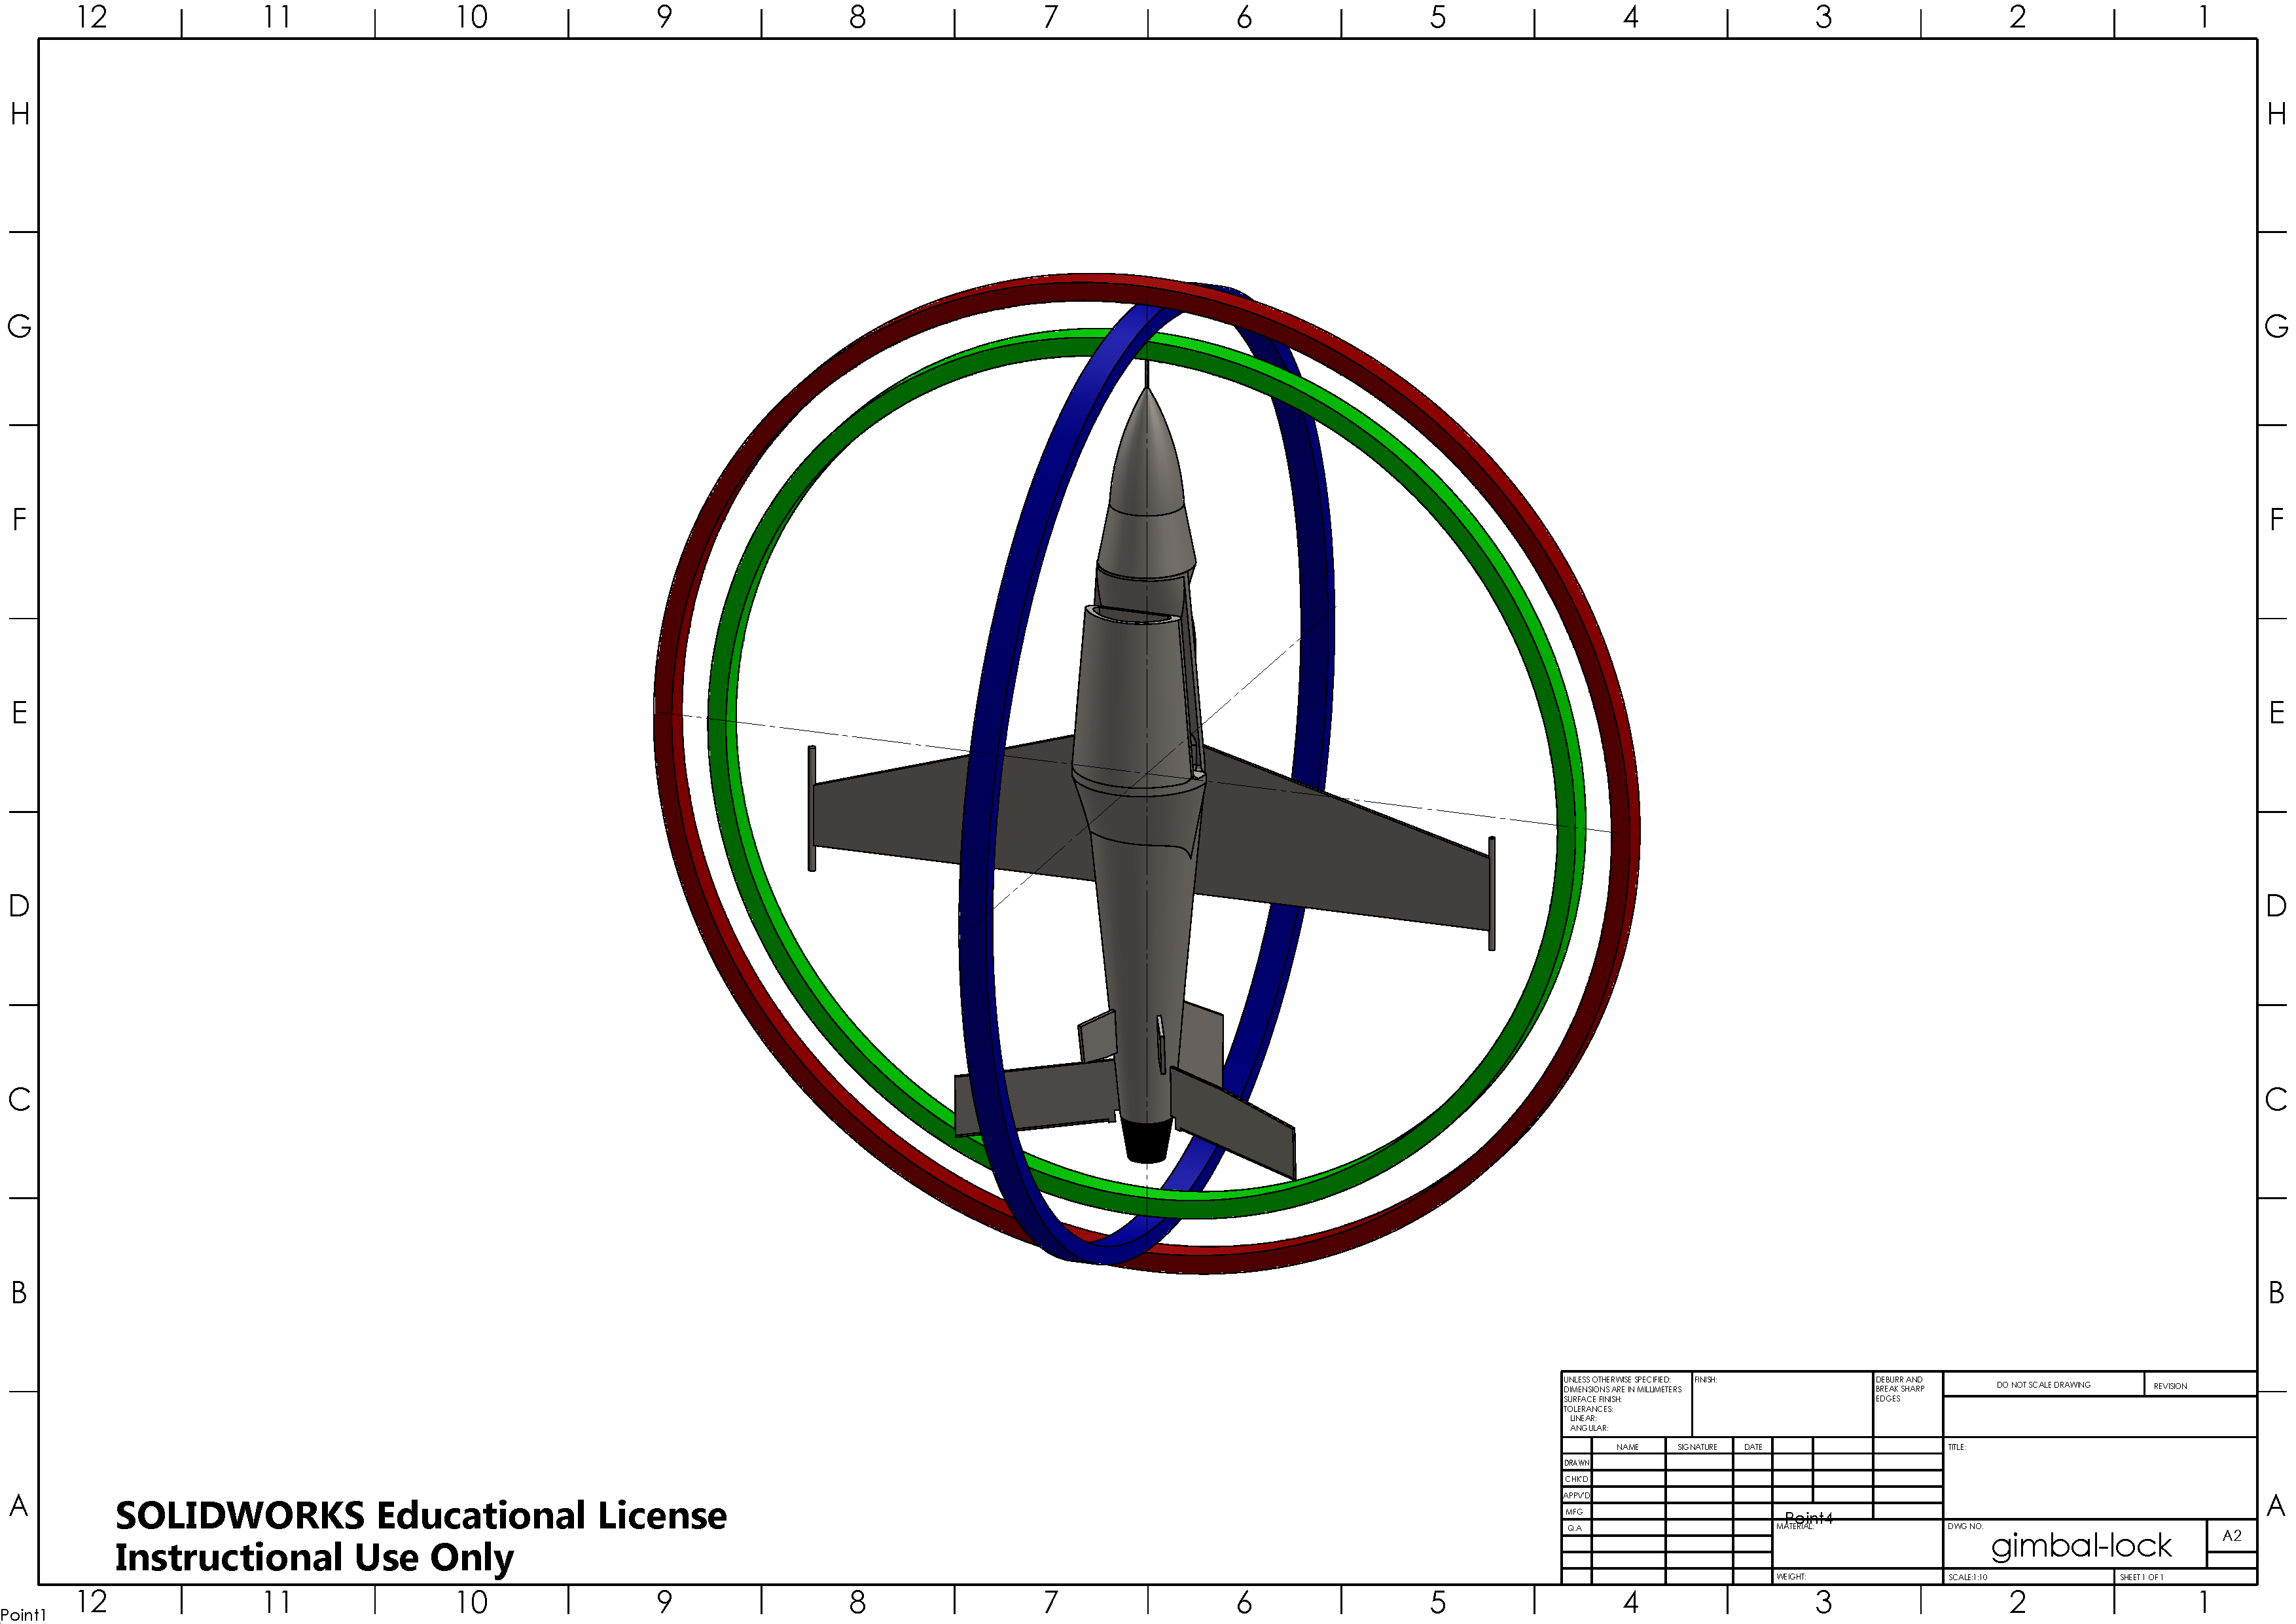
\includegraphics[clip, trim=16.5cm 8.5cm 16.5cm 6.7cm, width=0.93\textwidth]{pdfpages/gimbal-lock}
\caption{Locked gimbal with loss of DOF}
\label{fig:gimbal-lock}
\end{subfigure}
\caption{Mechanical gimbal lock}
\vspace{-10pt}
\end{figure} 
\par
What is clear physically is not necessarily as obvious mathematically. A loss of rank occurs in the Euler Matrix $\Psi(\eta)$, defined previously in Eq:\ref{eq:angular-rates.e} from Sec:\ref{subsec:proto.conventions.frames}. That relation between angular velocity, in the inertial frame or inversely in the body frame, and the angular rates of the Euler Angles has a determinant:
\begin{equation}\label{eq:euler-derivative}
\begin{bmatrix}
\dot{\phi}\\
\dot{\theta}\\
\dot{\psi}
\end{bmatrix}
=\begin{bmatrix}
1 & sin(\phi)tan(\theta) & cos(\phi)tan(\theta)\\
0 & cos(\phi) & -sin(\phi)\\
0 & sin(\phi)sec(\theta) & cos(\phi)sec(\theta)\\
\end{bmatrix}
\begin{bmatrix}
p\\
q\\
r
\end{bmatrix}
=\Phi(\eta)\omega_b~~~~\in\mathcal{F}^{v_1,v_2,I}
\end{equation}
\vspace{-2pt}
\begin{equation}
det\big(\Phi(\eta)\big)=cos(\phi)\big(cos(\phi)sec(\theta)\big)+sin(\phi)\big(\sin(\phi)sec(\theta)\big)=sec(\theta)
\end{equation}
\vspace{-6pt}
\begin{equation}
\therefore \underset{{\theta \rightarrow \pi /2}}{lim}|\Phi(\eta)|=sec(\theta)\rightarrow \infty
\end{equation}
The Euler matrix $\Phi(\eta)$ looses rank as $\theta\rightarrow\pi/2$ rad, loosing differentiability as well. The physical consequence of this is the loss of a degree of freedom. More specifically, if one looks at how the ZYX rotation (or transformation) matrices are formulated, from Eq:\ref{eq:rotationmatrix}.
\begin{subequations}
\begin{equation}
R_I^b(\eta)\triangleq R_z(\psi)R_y(\theta)R_x(\phi)=\begin{bmatrix}
c_\psi & -s_\psi & 0\\
s_\psi & c_\psi & 0\\
0 & 0 & 1
\end{bmatrix}
\begin{bmatrix}
c_\theta & 0 & s_\theta\\
0 & 1 & 0\\
-s_\theta & 0 & c_\theta
\end{bmatrix}
\begin{bmatrix}
1 & 0 & 0\\
0 & c_\phi & -s_\phi\\
0 & s_\phi & c_\phi
\end{bmatrix}
\end{equation}
\vspace{-3pt}
\begin{equation}
\therefore R_I^b(\eta)=\begin{bmatrix}
c_\psi c_\theta & c_\psi s_\theta s_\phi - s_\psi c_\phi & c_\psi s_\theta c_\phi + s_\psi s_\phi\\
s_\psi c_\theta & s_\psi s_\theta s_\phi + c_\psi c_\phi & s_\psi s_\theta  c_\phi - c_\psi s_\phi\\
-s_\theta & c_\theta s_\phi & c_\phi c_\theta\\
\end{bmatrix}
\end{equation}
In the case where $\theta=\pi/2$ rad, and using trigonometric double angles, the following can be reduced:
\begin{equation}
R_I^b(\eta)=\begin{bmatrix}
0 & c_\psi s_\phi - s_\psi c_\phi & c_\psi c_\phi + s_\psi s_\phi\\
0 & s_\psi s_\phi + c_\psi c_\phi & s_\psi c_\phi - c_\psi s_\phi\\
-1 & 0 & 0\\
\end{bmatrix}\Bigg|_{\theta=\pi/2}
\end{equation}
\vspace{-3pt}
\begin{equation}
=
\begin{bmatrix}
0 & s(\phi - \psi) & c(\phi - \psi)\\
0 & c(\phi - \psi) & s(\phi - \psi)\\
-1 & 0 & 0
\end{bmatrix}
\end{equation}
\vspace{-4pt}
\begin{equation}\label{eq:gimbal}
\therefore R_I^b(\eta)\big|_{\theta=\pi/2}\equiv R_{x'}(\phi-\psi)
\end{equation}
\end{subequations}
Where the resultant in Eq:\ref{eq:gimbal} represents an $\hat{X}'$-axis rotation in a new intermediate frame, post a $\pi/2$ rotation about the $\hat{Y}$-axis. Through trigonometric double angles a degree of freedom is lost at $\theta=\pi/2$, when both $\phi$ and $\psi$ effect the same angle.
%====================================================
\subsection{Quaternion Dynamics}
\label{subsec:dynamics.rigidbody.quaternion}
%====================================================
An algorithm proposed in \cite{euleranglesingularity} suggested a solution to avoid Euler Angle singularities. The heuristic proposed involved switching between sequence conventions (ZYX,ZYZ etc\ldots there are 12 in total) such that the singularity is always avoided. However the implementation of such an algorithm is cumbersome and compulationally exhaustive. Far more elegant is the use of \emph{quaternion} attitude representations in $\mathbb{R}^4$, used in \cite{rotationsequences,spacecraftattitutdequaternions} amongst others but most notably made popular by \cite{shoemake} for use in animation.
\par
A quaternion is analogous to a rotation matrix in that it represents an attitude difference between two reference frames. An $\mathbb{R}^3$ attitude is paramterized as one rotation $\theta$ about a single unit \emph{Euler} axis $\hat{u}$, demonstrated using the Rodriguez Formula in \cite{unwinding}. In brief, a quaternion consists of a scalar component $q_0$ and complex vector component $\vec{q}\in \mathbb{C}^3$ such that:
\begin{equation}
Q\triangleq 
\begin{bmatrix}
q_0 \\
\vec{q}
\end{bmatrix}
~~\in\mathbb{R}^4
\end{equation}
The relationship between an Euler angle rotation matrix $R_I^b(\eta)$ and a quaternion attitude $Q_b$ is given by the Rodriguez formula:
\begin{equation}\label{eq:rodriguez}
R_I^b(\eta)\equiv R(Q_b)\triangleq \mathbb{I}_{3\times 3}+2q_0[\vec{q}\hspace{2pt}]_\times+2[\vec{q}\hspace{2pt}]_\times\text{}^2
\end{equation}
Where $[.]_\times$ is the cross-product matrix, defined previously in Eq:\ref{eq:cross-product-matrix}, and $
mathbb{I}_{3\times 3}$ is an identity matrix as per convention. All quaternions, unless otherwise specified, are unit quaternions $Q\in\mathbb{Q}_u$. Quaternions with a unity magnitude ensure that rotational operations maintain the vector operand's magnitude. A unit quaternion is defined as follows:
\begin{equation}
\norm{Q}\triangleq\sqrt{{q_0}^2+\vec{q}\text{}\hspace{2pt}^2}=1
\end{equation}
Quaternion multiplication is distributive and associative, but not commutative. Specifically a quaternion multiplication operator is equivalent to the Hamilton product. For two quaternions, $Q$ and $P$:
\begin{subequations}
\begin{equation}
Q\otimes P = \begin{bmatrix}
q_0 \\
\vec{q}
\end{bmatrix}
\otimes
\begin{bmatrix}
p_0 \\
\vec{p}
\end{bmatrix}
\end{equation}
\begin{equation}\label{eq:quaternion-operator}
\triangleq\begin{bmatrix}
q_0p_0-\vec{q}\cdot\vec{p}\\
q_0\vec{p}+p_0\vec{q}+\vec{q}\times\vec{p}
\end{bmatrix}
\end{equation}
\begin{equation}\label{eq:quaternion-product}
=\underbrace{q_0 p_0 - \vec{q}\cdot \vec{p}}_{scalar}+\underbrace{p_0 \vec{q} + q_0 \vec{p} + \vec{q}\times\vec{p}}_{vector}
\end{equation}
\end{subequations}
Because the vector component of a quaternion is complex valued, it is natural that a quaternion complex conjugate $Q^*$ exists, defined:
\begin{equation}\label{eq:quaternion-conjugate}
Q^*\triangleq\begin{bmatrix}
q_0 \\
-\vec{q}~
\end{bmatrix}
\end{equation}
It follows that the fundamental quaternion identity is:
\begin{equation}
Q\otimes Q^* = \mathbb{I}_{4\times 4}
\end{equation}
A right handed quaternion rotation applied to some vector $\vec{\nu} \in\mathbb{R}^3$ involves multiplication by two unit quaternions $Q$ and its conjugate $Q^*$. 
\begin{equation}
\begin{bmatrix}
0 \\
\vec{\nu}\hspace{2pt}'
\end{bmatrix}
=Q\otimes
\begin{bmatrix}
0 \\
\vec{\nu}
\end{bmatrix}
\otimes Q^*
\end{equation}
Mostly, the zero scalar components are omitted in a rotation (\emph{or transformation}) operation, it is implied that vector operands are substituted with zero scalar quaternions.
\begin{equation}\label{eq:quaternion-rotation}
\vec{\nu}\hspace{2pt}'=Q \otimes (\vec{\nu}\hspace{2pt}) \otimes Q^*
\end{equation} 
In the case of rigid body attitude parametrization using quaternions, $Q_b$ is the quaternion which represents the difference between body and inertial frames $\mathcal{F}^b$ and $\mathcal{F}^I$ respectively. A quaternion operator is equivalent to a rotation matrix operation, for some vector $\vec{\nu}_I\in\mathcal{F}^I$;
\begin{equation}
\vec{\nu}_b=R_I^b(\eta)\vec{\nu}_I \underset{Q}{\iff} Q_b \otimes (\vec{\nu}_I) \otimes Q_b^*~~~~\in\mathcal{F}^b
\end{equation}
Since quaternions are non-commutative, the construction of a body quaternion $Q_b$ from an Euler angle set $\vec{\eta}$ is \emph{sequence dependent}. Euler angles, despite being singular, are conceptually simpler for describing a body's orientation. A ZYX sequenced body quaternion $Q_b$ relative to the inertial frame can be constructed from its Euler angle counterparts using:
\begin{equation}\label{eq:quaternion-sequence}
Q_b\triangleq Q_z\otimes Q_y\otimes Qx=\begin{bmatrix}
cos(\psi/2)\\
0\\
0\\
sin(\psi/2)
\end{bmatrix}
\otimes
\begin{bmatrix}
cos(\theta/2)\\
0\\
sin(\theta/2)\\
0
\end{bmatrix}
\otimes
\begin{bmatrix}
cos(\phi/2)\\
sin(\phi/2)\\
0\\
0
\end{bmatrix}
\end{equation}
A quaternion's time derivative, defined in \cite{fullquaternion}, with $Q_\omega$ being a quaternion with a vector component equal to angular velocity $\vec{\omega}_{b/I}$ and a zero scalar component, is:
\begin{subequations}\label{eq:quaternion-deriv}
\begin{equation}
\frac{d}{dt}Q_b\triangleq\frac{1}{2}Q_b\otimes Q_{\omega}=\frac{1}{2}Q_b\otimes\vec{\omega}_b
\end{equation}
\vspace{-12pt}
\begin{equation}
=\begin{bmatrix}
-\frac{1}{2}\vec{q}\hspace{2pt}^{T} \vec{\omega}_b\\
\frac{1}{2}\big([\vec{q}\hspace{2pt}]_\times+q_0\mathbb{I}\big)\vec{\omega}_b
\end{bmatrix}
\end{equation}
\end{subequations}
Using quaternions to represent attitudes negates the need for an Euler Matrix, $\Phi(\eta)$ from Eq:\ref{eq:angular-rates.f}, to represent attitudes and their rates. A body quaternion is fully defined in the inertial frame with respect to the body frame or inversely so. The first quaternion time derivative replaces angular velocity rate differentials in Eq:\ref{eq:states.a} and Eq:\ref{eq:states.c} respectively:
\begin{subequations}
\begin{equation}
\dot{\mathcal{E}}=R_b^I(-\eta)\vec{v}_b~~\in\mathcal{F}^I\underset{Q}{\iff}Q_b(-\eta)\otimes\vec{v}_b\otimes Q_b^*(-\eta)=Q_b^*\otimes \vec{v}_b \otimes Q_b
\end{equation}
\vspace{-14pt}
\begin{equation}
\dot{\eta}\triangleq\Phi(\eta)\vec{\omega}_b~~\in\mathcal{F}^{v2,v1,I}\underset{Q}{\iff}\dot{Q}_b=\frac{1}{2}Q_b\otimes \vec{\omega}_b
\end{equation}
\end{subequations}
Second order time derivatives for quaternion acceleration are not as useful as their higher order, velocity counterparts. The second order derivative is provided here for the sake of completeness. If at all possible, quaternion accelerations are avoided due to their complexity. The quaternion analogue for angular acceleration Eq:\ref{eq:rigid-frame.b}, dependent on net torque acting on a body $\vec{\tau}_{\mu}$, is given by:
\begin{equation}
\ddot{Q}\big(\dot{Q},Q,t)\triangleq\dot{Q}\otimes Q^* \otimes \dot{Q}+\frac{1}{2}Q\otimes \big[J_b^{-1}(\vec{\tau}_{\mu}-4(Q^*\otimes \dot{Q})\times(J_b(Q^*\otimes \dot{Q}))\big]
\end{equation}
An Euler angle attitude error state, used for control input, is defined as the subtracted error between a desired and an existing attitude orientation; $\vec{\eta}_d\in\mathcal{F}^d$ and $\vec{\eta}_b\in\mathcal{F}^b$ respectively. Where $\vec{\eta}_d$ is some attitude setpoint produced from a trajectory generator and both Euler sets are in shared frames.
\begin{equation}\label{eq:euler-error}
\vec{\eta}_e\triangleq\vec{\eta}_d-\vec{\eta}_b
\end{equation}
Quaternion attitude control and its stability goals are expanded upon subsequently in Sec:\ref{subsec:control.attitude.problem}. In contrast with Eq:\ref{eq:euler-error}, a quaternion attitude error is a multiplicative term defined as the difference between two quaternions $Q_d$ and $Q_b$:
\begin{equation}\label{eq:quaternion-error}
Q_e\triangleq Q_b^*\otimes Q_d
\end{equation}
%====================================================
\subsection{Quaternion Unwinding}
\label{subsec:dynamics.rigidbody.unwinding}
%====================================================
Although quaternions are indeed better than their Euler angle attitde counterparts and lack the associated singularity they do contain one caveat. Becuase a quaternion $Q=[q_0~\vec{q}\hspace{2pt}]^T$ represents a body's attitude in $\mathbb{R}^3$ using $\mathbb{R}^4$ there is an infinite coverage of attitude states, \cite{unwinding}. 
\par
Each unit quaternion, stemming from Euler-Rodriguez theorem, represents a single Euler-axis rotation of $\theta$ about a unit axis $\hat{u}$ such that:
\begin{equation}\label{eq:quaternion-euler-axis}
Q=\begin{bmatrix}
q_0\\
\vec{q}
\end{bmatrix}\triangleq
\begin{bmatrix}
cos(\theta/2)\\
sin(\theta/2)\hat{u}
\end{bmatrix}
\end{equation}
That rotation is applied with a quaternion operator, Eq:\ref{eq:quaternion-rotation}. For every attitude state in 3-D there exist two unique quaternions which correspond to the same orientation, differing by their rotational direction about the Euler-axis. The rotation angle $\theta$ about the Euler-axis $\hat{u}$ is reciprocal in that $\theta=\theta + 2k\pi,~k\in\mathbb{N}$. There are then two definitions for $Q_b$:
\begin{subequations}
\begin{equation}
Q_b =
\begin{bmatrix}
cos(\theta/2)\\
sin(\theta/2)\hat{u}
\end{bmatrix}
\end{equation}
\vspace{-6pt}
\begin{equation}
Q_b=\begin{bmatrix}
cos(\pi - \theta/2)\\
sin(\pi - \theta/2)\hat{u}
\end{bmatrix}
=
\begin{bmatrix}
-cos(\theta/2)\\
sin(\theta/2)\hat{u}
\end{bmatrix}
\end{equation}
\vspace{-4pt}
\begin{equation}\label{eq:euler-quaternion}
\therefore\vec{\eta}\in\mathbb{R}^3\underset{Q}{\iff}\begin{bmatrix}
\pm q_0\\
\vec{q}
\end{bmatrix}
\in\mathbb{R}^4
\end{equation}
\end{subequations}
Eq:\ref{eq:euler-quaternion} asserts that for each attitude in $\mathbb{R}^3$ there are \emph{two} corresponding quaternions in $\mathbb{R}^4$; $[\pm q_0~\vec{q}~]^T$. A consequence of this is that two possible error state trajectories exist for every attitude difference. Both a clockwise $+\theta$ and an anticlockwise $2\pi-\theta$ rotation points to the same quaternion attitude error state. This could lead to an erroneous and unnecessary ``unwinding" of a complete counter revolution. So for attitude controllers the requirement is that for positive and negative quaternion scalars the control input is consistent:
\begin{equation}
\vec{\tau}_d=h([q_0~\vec{q}\hspace{2pt}]^T,t)\equiv h([-q_0~\vec{q}\hspace{2pt}]^T,t)
\end{equation}
Or more simply that $Q_e\triangleq[|q_0|~\vec{q}\hspace{2pt}]^T$. The simplest solution adhering to that constraint, which is often used, is to neglect the quaternion scalar component altogether. Using a reduced error state, only the quaternion error vector as an argument for the control law; $h(\vec{q}_e,t)$. Such a solution is an oversimplification and would only ever be locally stable. 
\par
An alternative is to use only the absolute quaternion scalar, which ensures the error state represents a right-handed (clockwise) rotation and not necessarily the shortest path. If the resolution of trajectory coordinates generated is sufficiently fine the control plant will not encounter a problem.
\par
One proposal presented in \cite{nonlinearquadcopter} suggested using a \emph{signum} operator to design the controller coefficient sign for the desired virtual angular velocity, $\vec{\omega}_d$ control plant input. 
\begin{subequations}\label{eq:signum-unwinding}
\begin{equation}
\vec{\omega}_d=\frac{2}{\Gamma_1}sgn(q_0)\vec{q}
\end{equation}
With $\Gamma_1$ being a proportional error coefficient and signum defining the operator's sign:
\begin{equation}
sgn(q_0)\triangleq
\begin{cases}\begin{array}{ll}
1 & ~~q_0\geq 0\\
-1 & ~~q_0< 0\\
\end{array}
\end{cases}
\end{equation}
\end{subequations}
Eq:\ref{eq:signum-unwinding} was shown to be asymptotically stable but only locally in the case where the Euler-axis angle is constrained; $\theta\leq \pm\pi$. That control law  would still need the control torques to be calculated from that angular velocity $\vec{\omega}_d$ setpoint using Eq:\ref{eq:states.d}.
\par
In \cite{intelligentbackstep}, the authors used a backstepping controller with a trajectory using the absolute quaternion scalar. The resultant was a global asymptotically stable control law which tracked quaternion setpoints for a satellite's attitude. That satellite's stability proof was, however, difficult given the hybrid nature of the resulting equations. Controllers presented in Sec:\ref{subsec:control.attitude.nonlinear} all incorporate \emph{signed} quaternion scalars into the control law; the trajectory generation is assumed to specify the preferred quaternion rotational sense.
\newpage
%====================================================
\section{Multibody Nonlinearities}
\label{sec:dynamics.nonlinearities}
%====================================================
The unique component of the prototype's design which facilitates redirection of a propeller's thrust vector (Eq:\ref{eq:motor-module-force-redirect} and Sec:\ref{subsec:proto.design.actuation}) is also what makes finding the complete equations of motion drastically more complex. The relative (revolute) motion within the multibody system results in torque responses opposing those angular accelerations. Such induced responses, if left unmodelled, would almost definitely destabilize the attitude plant. Unmodelled inertia rate responses are shown to be destabilizing in \cite{inertiaspin}. Typically multibody dynamics are solved and simulated as a series of interacting torque and force constraints. There are different schools of thought on the subject, each proposing methodologies for stepping through the systems dynamics; \emph{e.g} Implicit Euler integration\cite{physicallybased,multibodydynamics}\ldots
\par
The prototype investigated here is a multibody system connected with revolute joints, which permit a single degree of relative rotation between each connected rigid body. There are no translational degrees of freedom between each body. Opposed to the angular accelerating actuator action on a body are \emph{gyroscopic} and \emph{inertia} Newtonian torque responses. The responses from each body are solved independently and those excitation induced torque constraints are introduced as additive external torques to the dynamic model derived in Sec:\ref{subsec:dynamics.rigidbody.lagrange}. A distinction must be made between torque responses here and those previously in Eq:\ref{eq:states.d}. Recalling the classical differential equation of angular motion already derived:
\begin{equation}\label{eq:angular-multibody}
\dot{\vec{\omega}}_b=J_b^{-1}\big(-\vec{\omega}_b\times J_b\vec{\omega}_b+\vec{\tau}_\mu\big)~~~~\in\mathcal{F}^b
\end{equation}
Eq:\ref{eq:angular-multibody} treats the entire body as rigid; included terms are as a result of the entire multibody's collective motion. What follows is an extension of that attitude state to incorporate relative movements between each connected body. The objective here is to model the multibody dynamic system with clear responses induced from servo rotations of inner and middle ring bodies, $\Delta\lambda_i$ and $\Delta\alpha_i$ respectively. The subsequent derivations are Lagrangian analytical dynamics applied to the multibody system under consideration. For the purposes of this derivation it is assumed that no potential energy can be stored within the structure from material flexure. The only potential energy contribution is as a result of gravitational potential energy. Moreover, each connected body is first solved as a closed energy system to ascertain the relative rotational response which is then incorporated in the overall multibody system.
\par
Alternatively the net dynamics could indeed be derived from a Lagrangian for the \emph{entire} 13 body dynamic system. Where those connected bodies are; four rotor/propeller bodies (Fig:\ref{fig:inertia-prop}), four inner ring bodies (Fig:\ref{fig:inertia-inner}), four middle ring bodies (Fig:\ref{fig:inertia-middle}) and finally the frame structure (Fig:\ref{fig:inertia-frame}) each with six degrees of freedom. Constraints on the assembly's joints would eventually reduce the degrees of freedom and simplify solving for net responses. The purpose here is to model the body's response to changes in the actuation servos' positions $\Delta\lambda_i$ and $\Delta\alpha_i$ so independent bodies are analyzed first. The final result is, in fact, a Lagrangian for those collective thirteen bodies, whose partial derivative with respect to the net angular velocity relative to the inertial frame $\partial\vec{\omega}_b$ produces the net torque acting on the system.
%====================================================
\subsection{Relative Rotational Gyroscopic \& Inertial Torques}
\label{subsec:dynamics.nonlinearities.gyrotorques}
%====================================================
\emph{\color{gray}Rotation matrices are used in the following derivations owing to the fact that induced torque responses are dependent on transformed rotational inertias. Quaternions, as mentioned in Sec:\ref{sec:proto.inertia}, are ill-suited to inertia transformations.}
\par
Each of the four motor modules are symmetrical and so the induced torque response characteristics from one module can be extrapolated simply through a $\hat{Z}_b$ reference frame rotation. Each motor module is positioned relative to the body frame's center of motion $\vec{\mathbf{O}}_b$, as in Fig:\ref{fig:body-frame}. Because each relative rotation from the actuator set $u\in\mathbb{U}$ is actuated separately and upon a different body, their responses are calculated independently too.
\par
Drawing again from Lagrangian theory and considering only the angular energy component for the inner ring assembly attached to frame $\mathcal{F}^{M_i}$. There is no relative translational motion between each connected body and the origin of \emph{motion} $\vec{\mathbf{O}}_b$, the center of the body frame $\mathcal{F}^b$ from Fig:\ref{fig:body-frame} and Fig:\ref{fig:inertia-center}. Relative velocity of each body's center of gravity with respect to $\vec{\mathbf{O}}_b$, from each rotational actuation, is small in relation to the net vehicle's translational velocity. So translational kinetic energy for each module is treated as an extension of body's net kinetic energy in Eq:\ref{eq:3.7a} and assumed to be independent of any actuator's position. The following is with regards to the $i^{th}$ motor module, numerical subscripts are implied.
\begin{figure}[htbp]
\vspace{-12pt}
\centering
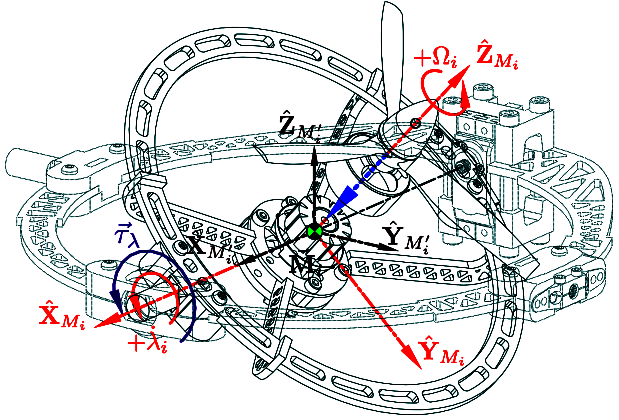
\includegraphics[width=0.8\textwidth]{figs/response-inner}
\vspace{-8pt}
\caption{Exploded inner ring inertial bodies for $\vec{\tau}_\lambda(\lambda_i)$}
\label{fig:response-inner}
\vspace{-16pt}
\end{figure}
\par
Deriving dynamic responses for changes in the $\lambda_i$ servo, acting on the inner ring frame $\mathcal{F}^{M_i}$ relative to the middle ring frame $\mathcal{F}^{M_i'}$, requires a relative path coordinate to be defined. The only path variable between the two frames is that servo's rotational position $\lambda_i$ about the $\hat{X}_{M_i}$ axis. Path coordinates $\vec{\mathbf{u}}(t)=\begin{bmatrix}\lambda_i&0&0\end{bmatrix}^T$ are then used to construct the inner ring's closed energy system Lagrangian with respect the middle ring frame $\mathcal{L}_{n/m}\in\mathcal{F}^{M_i'}$.
\par
The inner ring assembly consists of two separate bodies, exploded in Fig:\ref{fig:response-inner}, each has a relative rotational motion and independent kinetic energies. Those bodies are; the rotor assembly with an inertia $J_{r}$ defined earlier in Eq:\ref{eq:prop-inertia} and the inner ring which has an inertia $J_{ir}$ \emph{without including} the rotor assembly. Reiterating that the rotor's inertia $J_r$ is constant with respect to the propeller's rotational velocity $\Omega_i$, that inner ring inertia is given by:
\begin{equation}
J_{ir}\triangleq J_{n}-J_{r}
\end{equation} 
Where $J_n$ is the net inertia for the inner ring assembly, explicitly defined in Eq:\ref{eq:inertia.inner}. The rotor assembly has an angular velocity $\vec{\omega}_{r/m}$ relative to the middle ring frame $\mathcal{F}^{M_i'}$ due to the BLDC motor's rotation $\Omega_i$ and the inner ring's servo rate $\dot{\lambda}_i$:
\begin{equation}\label{eq:angular-rot}
\vec{\omega}_{r/m}\triangleq R_x(\lambda_i)\vec{\Omega}_i+\dot{\vec{\lambda}}_i~~~~\in\mathcal{F}^{M_i'}
\end{equation}
With the propeller's angular velocity vector about the inner ring frame's $\hat{Z}_{M_i}$ axis $\vec{\Omega}_i\triangleq\begin{bmatrix}0 & 0 & \Omega_i\end{bmatrix}^T\in\mathcal{F}^{M_i}$ and measured in $[\text{rad.s}^{-1}]$ not in \emph{revolutions per second}. The servo position is defined as a vector in the $\hat{X}_{M_i'}$ axis projected as $\vec{\lambda}_i\triangleq \lambda_i\cdot\hat{X}_{M_i'}=\begin{bmatrix}\lambda_i & 0 & 0\end{bmatrix}^T$ measured in $[\text{rad}]$. Next, the inner ring's angular velocity $\vec{\omega}_{n/m}$ relative to the middle ring $\mathcal{F}^{M_i'}$ is only as a result of $\dot{\lambda}_i$:
\begin{equation}\label{eq:angular-inner}
\vec{\omega}_{n/m}\triangleq\frac{d}{dt}(\vec{\lambda}_i)=\dot{\vec{\lambda}}_i~~~~\in\mathcal{F}^{M_i'}
\end{equation}
\par
The Lagrangian for the inner ring's closed system energy $\mathcal{L}_{n/m}$, in the middle ring frame $\mathcal{F}^{M_i'}$, consists purely of rotational kinetic energy from angular velocities described in Eq:\ref{eq:angular-rot} and Eq:\ref{eq:angular-inner}. Stored gravitation potential energy as a result of the rotated center of mass for the inner ring is omitted here as it is already included in Eq:\ref{eq:grav-torque} and is shown to simplify out subsequently in Eq:\ref{eq:3.109} when considering the entire system as a whole. The inner ring's Lagrangian is:
\begin{subequations}\label{eq:lagrange-inner}
\begin{equation}\label{eq:lagrange-inner.a}
\mathcal{L}_{n/m}=\frac{1}{2}\vec{\omega}_{r/m}\text{}^T\big(J_{r}'\big)\vec{\omega}_{r/m}+\frac{1}{2}\vec{\omega}_{n/m}\text{}^T\big(J_{ir}'\big)\vec{\omega}_{n/m}
\end{equation}
Both inertias for the rotor and inner ring bodies, $J_r$ and $J_{ir}$ respectively, are transformed to align with the middle ring frame $\mathcal{F}^{M_i'}$ using an $R_x(\lambda_i)$ rotation to align with the middle ring's frame $\mathcal{F}^{M_i'}$.
\begin{equation}
J_r'= R_x(\lambda_i)\big(J_r\big)R_x^{-1}(\lambda_i)~~\text{and}~~J_{ir}'= R_x(\lambda_i)\big(J_{ir}\big)R_x^{-1}(\lambda+i)
\end{equation}
Then expanding the Lagrangian $\mathcal{L}_{n/m}$ in Eq:\ref{eq:lagrange-inner.a} with the above definitions for transformed inertias and relative angular velocities $\vec{\omega}_{r/m}$ and $\vec{\omega}_{n/m}$ yields:
\begin{multline}\label{eq:lagrange-inner.b}
\therefore\mathcal{L}_{n/m}=\frac{1}{2}\Big(R_x(\lambda_i)\vec{\Omega}_i+\dot{\vec{\lambda}}_i\Big)^T\big(R_x(\lambda_i)\big(J_{r}\big)R_x^{-1}(\lambda_i)\big)\Big(R_x(\lambda_i)\vec{\Omega}_i+\dot{\vec{\lambda}}_i\Big)\\+\frac{1}{2}\dot{\vec{\lambda}}_i^{\hspace{2pt}T}\big(R_x(\lambda_i)\big(J_{ir}\big)R_x^{-1}(\lambda_i)\big)\dot{\vec{\lambda}}_i
\end{multline}
\end{subequations}
Reiterating, $J_{ir}$ is the inner ring's inertia independent from the rotor assembly $J_{r}$. Recalling the Euler-Lagrange formulation from Eq:\ref{eq:euler-lagrange} using path coordinates $\vec{\mathbf{u}}(t)$ for the inner ring frame $\mathcal{F}^{M_i}$ relative to the middle ring frame $\mathcal{F}^{M_i'}$. The generalized (torque) forces $\vec{\mathbf{U}}$ acting on the middle ring are then:
\begin{equation}\label{eq:euler-lagrange-inner}
\vec{\mathbf{U}}(\lambda_i)=\frac{d}{dt}\bigg(\frac{\partial \mathcal{L}_{n/m}}{\partial \dot{\vec{\mathbf{u}}}}\bigg)-\frac{\partial \mathcal{L}_{n/m}}{\partial \vec{\mathbf{u}}}~~~~\in\mathcal{F}^{M_i'}
\end{equation}
Considering first the partial derivative of the Lagrangian $\mathcal{L}_{n/m}$ but with respect to the generalized path coordinates $\partial\vec{\mathbf{u}}$. The latter part of the Euler-Lagrange formulation with respect to the inner ring in Eq:\ref{eq:euler-lagrange-inner} then expands from the differential product rule:
\begin{multline}\label{eq:euler-lagrange-inner-partial}
\frac{\partial\mathcal{L}_{n/m}}{\partial\vec{\mathbf{u}}}=\frac{1}{2}\Bigg[\bigg(\frac{\partial}{\partial\vec{\lambda}_i}R_x(\lambda_i)\vec{\Omega}_i\bigg)^T\big(J_r'\big)\Big(R_x(\lambda_i)\vec{\Omega}_i+\dot{\vec{\lambda}}_i\Big)+\Big(R_x(\lambda_i)\vec{\Omega}_i+\dot{\vec{\lambda}}_i\Big)^T\bigg(\frac{\partial}{\partial\vec{\lambda}_i}J_r'\bigg)\Big(R_x(\lambda_i)\vec{\Omega}_i+\dot{\vec{\lambda}}_i\Big)
\\
+\Big(R_x(\lambda_i)\vec{\Omega}_i+\dot{\vec{\lambda}}_i\Big)\big(J_r'\big)\bigg(\frac{\partial}{\partial\vec{\lambda}_i}R_x(\lambda_i)\bigg)\Bigg]+\frac{1}{2}\dot{\vec{\lambda}}_i^{\hspace{2pt}T}\bigg(\frac{\partial}{\partial\vec{\lambda}_i}J_{ir}'\bigg)\dot{\vec{\lambda}}_i
\end{multline}
Partial derivatives with respect to the chosen path variable, $\partial\vec{\mathbf{u}}=\partial\vec{\lambda}_i$ in Eq:\ref{eq:euler-lagrange-inner-partial}, only act on rotation matrices $R_x(\lambda_i)$. For the partial derivative of a generalized rotation matrix $R_{\hat{u}}(\theta)$, whose equation is given by Eq:\ref{eq:genrotationmatrix}, derived with respect to its angular operand $\partial\theta$:
\begin{subequations}\label{eq:partial-rotation}
\begin{equation}\label{eq:rotation-partial}
\frac{\partial}{\partial\theta} R_{\hat{u}}(\theta)\triangleq [\hat{u}]_\times R_{\hat{u}}(\theta)
\end{equation}
Where $[\hat{u}]_\times$ in Eq:\ref{eq:rotation-partial} is the cross product matrix from Eq:\ref{eq:cross-product-matrix} of the unit vector $\hat{u}$ in the direction of the axis about which the rotation matrix applies its rotation. In the case of an $\hat{X}$ axis rotation matrix, as in Eq:\ref{eq:euler-lagrange-inner-partial}, the expanded partial derivative is:
\begin{equation}\label{eq:rotation-xaxis-partial}
\frac{\partial}{\partial\vec{\lambda}_i}R_x(\lambda_i)\triangleq [\hspace{2pt}\hat{\i}\hspace{2pt}]_\times R_x(\lambda_i) = 
\begin{bmatrix}
0 & 0 & 0\\
0 & 0 & -1\\
0 & 1 & 0
\end{bmatrix}R_x(\lambda_i)
\end{equation}
And similarly, the same partial derivative of a rotation matrix transpose $R_x^T(\lambda_i)$ as follows:
\begin{equation}\label{eq:rotation-xaxis-transpose-partial}
\frac{\partial}{\partial\vec{\lambda}_i}R_x^T(\lambda_i)\triangleq -[\hspace{2pt}\hat{\i}\hspace{2pt}]_\times R_x^T(\lambda_i)=\begin{bmatrix}
0 & 0 & 0\\
0 & 0 & 1\\
0 & -1 & 0
\end{bmatrix} R_x^T(\lambda_i)
\end{equation}
\end{subequations}
Applying Eq:\ref{eq:partial-rotation} to the Lagrangian's partial derivative in Eq:\ref{eq:euler-lagrange-inner-partial} reduces and simplifies:
\begin{multline}\label{eq:euler-lagrange-inner-partial}
\frac{\partial\mathcal{L}_{n/m}}{\partial\vec{\mathbf{u}}}=\frac{1}{2}\bigg[\Big([\hspace{2pt}\hat{\i}\hspace{2pt}]_\times R_x(\lambda_i)\vec{\Omega}_i\Big)^T\big(R_x(\lambda_i)\big(J_{r}\big)R_x^{-1}(\lambda_i)\big)\Big(R_x(\lambda_i)\vec{\Omega}_i+\dot{\vec{\lambda}}_i\Big)
\\
+\Big(R_x(\lambda_i)\vec{\Omega}_i+\dot{\vec{\lambda}}_i\Big)^T\big([\hspace{2pt}\hat{\i}\hspace{2pt}]_\times R_x(\lambda_i)\big(J_r\big)R_x^{-1}(\lambda_i)-R_x(\lambda_i)\big(J_r\big)[\hspace{2pt}\hat{\i}\hspace{2pt}]_\times R_x^{-1}(\lambda_i)\big)\Big(R_x(\lambda_i)\vec{\Omega}_i+\dot{\vec{\lambda}}\Big)
\\
+\Big(R_x(\lambda_i)\vec{\Omega}_i+\dot{\vec{\lambda}}\Big)^T\big(R_x(\lambda_i)\big(J_r\big)R_x^{-1}(\lambda_i)\big)\Big([\hspace{2pt}\hat{\i}\hspace{2pt}]_\times R_x(\lambda_i)\vec{\Omega}_i\Big)\bigg]
\\
+\frac{1}{2}\dot{\vec{\lambda}}_i^{\hspace{2pt}T}\big([\hspace{2pt}\hat{i}\hspace{2pt}]_\times R_x(\lambda_i)\big(J_{ir}\big)R_x^{-1}(\lambda_i)-R_x(\lambda_i)\big(J_r\big)[\hspace{2pt}\hat{\i}\hspace{2pt}]_\times R_x(\lambda_i)\big)\dot{\vec{\lambda}}_i=0
\end{multline}
Fortunately the quadratic form of kinetic energies included in Eq:\ref{eq:lagrange-inner.b} resulted in symmetrical partial derivatives of rotation matrices in Eq:\ref{eq:euler-lagrange-inner-partial} simplifying out. So, after some mathematics it follows that partial derivatives of the Lagrangian in Eq:\ref{eq:lagrange-inner} with respect to $\vec{\mathbf{u}}$ are negligible; or that $\partial\mathcal{L}_{n/m}/\partial\vec{\mathbf{u}}= 0$. Only the partial derivatives with respect to the path rate $\dot{\vec{\mathbf{u}}}$ remain:
\begin{equation}\label{eq:3.42b}
\vec{\mathbf{U}}(\lambda_i)=\frac{d}{dt}\bigg(\frac{\partial \mathcal{L}_{n/m}}{\partial \dot{\vec{\mathbf{u}}}}\bigg)=\frac{d}{dt}\bigg(\big(J_{r}'\big)\Big(R_x(\lambda_i)\vec{\Omega}_i+\dot{\vec{\lambda}}_i\Big)+\big(J_{ir}'\big)\dot{\vec{\lambda}}_i\bigg)
\end{equation}
Transformed rates of change for inertias $\dot{J}_r'$ and $\dot{J}_{ir}'$ must first be defined before evaluating the simplified Lagrangian derivative in Eq:\ref{eq:3.42b}. Derivatives of those inertias cannot be separated by time scale from the remainder of Eq:\ref{eq:3.42b} given that $\dot{\lambda}_i$ determines both inertia rates of change $\dot{J}_r'$ and $\dot{J}_{ir}'$ but is also a component of the kinetic energy in Eq:\ref{eq:lagrange-inner.b}.
\par
Starting with the general case; for some transformed inertia $J$ to be aligned relative to a frame $\mathcal{F}^b$ where the inertia is originally defined with respect to a frame $\mathcal{F}^a$. If the two frames differ by some rotation angle $\theta$ about an Euler axis $\hat{u}$, the generalized rotation matrix from frame $\mathcal{F}^a$ to $\mathcal{F}^b$ is given by $R_{\hat{u}}(\theta)$ from Eq:\ref{eq:rotationoperator}. The transformed inertia is then calculated as:
\begin{subequations}
\begin{equation}
J'=R_{\hat{u}}(\theta)\big(J\big)R_{\hat{u}}^{-1}(\theta)
\end{equation}
Which, from the product rule and the rotation matrix time derivative definition previously in Eq:\ref{eq:rotation-matrix-derivative}, has a rate of change as a result of the angular velocity $\dot{\theta}$:
\begin{equation}
\dot{J}'=\frac{d}{dt}\Big(R_{\hat{u}}(\theta)\big(J\big)R_{\hat{u}}^{-1}(\theta)\Big)
\end{equation}
\vspace{-10pt}
\begin{equation}
=\frac{d}{dt}\Big(R_{\hat{u}}(\theta)\Big)\big(J\big)R_{\hat{u}}^{-1}(\theta)+R_{\hat{u}}(\theta)\Big(\frac{d}{dt}\big(J\big)\Big)R_{\hat{u}}^{-1}(\theta)+R_{\hat{u}}(\theta)\big(J\big)\frac{d}{dt}\Big(R_{\hat{u}}^{-1}(\theta)\Big)
\end{equation}
\vspace{-6pt}
\begin{equation}\label{eq:inertial-rate-def}
=[\dot{\vec{\theta}}\hspace{2pt}]_\times R_{\hat{u}}(\theta)\big(J\big)R_{\hat{u}}^{-1}(\theta)+R_{\hat{u}}(\theta)\big(\dot{J}\big)R_{\hat{u}}^{-1}(\theta)-R_{\hat{u}}(\theta)\big(J)[\dot{\vec{\theta}}\hspace{2pt}]_\times R_{\hat{u}}^{-1}(\theta)
\end{equation}
\end{subequations}
Where $\dot{\vec{\theta}}\triangleq\dot{\theta}\cdot\hat{u}$ is the projcted angular velocity vector between the two frames. In most cases, the inertia will not be changing in its principle frame, or rather that $\dot{J}=0$. Both the rotor assembly and inner ring inertias are constant in their principle frames. The transformed inertias then have the following derivatives; first for the rotor assembly:
\begin{subequations}\label{eq:rotor-deriv}
\begin{equation}
\dot{J}_r'=\frac{d}{dt}\Big(R_x(\lambda_i)\big(J_r\big)R_x^{-1}(\lambda_i)\Big)
\end{equation}
\vspace{-10pt}
\begin{equation}
=[\dot{\vec{\lambda}}_i]_\times R_x(\lambda_i)\big(J_r\big)R_x^{-1}(\lambda_i)-R_x(\lambda_i)\big(J_r\big)[\dot{\vec{\lambda}}_i]_\times R_x^{-1}(\lambda_i)
\end{equation}
\end{subequations}
Similarly for the inner ring's transformed inertia rate $\dot{J}_{ir}'$ again without the rotor's contribution:
\begin{subequations}\label{eq:inner-deriv}
\begin{equation}
\dot{J}_{ir}'=\frac{d}{dt}\Big(R_x(\lambda_i)\big(J_{ir}\big)R_x^{-1}(\lambda_i)\Big)
\end{equation}
\vspace{-12pt}
\begin{equation}
=[\dot{\vec{\lambda}}_i]_\times R_x(\lambda_i)\big(J_{ir}\big)R_x^{-1}(\lambda_i)-R_x(\lambda_i)\big(J_{ir}\big)[\dot{\vec{\lambda}}_i]_\times R_x^{-1}(\lambda_i)
\end{equation}
\end{subequations}
Substituting those transformed inertia rates of change into Eq:\ref{eq:3.42b} and using Reynolds transportation theorem, Eq:\ref{eq:reynolds} for a vector's derivative in a rotating reference frame, the product rule then yields:
\begin{multline}
\frac{d}{dt} \bigg(\frac{\partial \mathcal{L}_{n/m}}{\partial \dot{\vec{\mathbf{u}}}}\bigg)=\Big[\big(\dot{J}_r'\big)\big(R_x(\lambda_i)\vec{\Omega}_i + \dot{\vec{\lambda}}_i\big)+\big(J_{r}'\big)R_x(\lambda_i)\dot{\vec{\Omega}}_i+\vec{\omega}_{r/m}\times \big(J_{r}'\big)R_x(\lambda_i)\vec{\Omega}_i+\big(J_{r}'\big)\ddot{\vec{\lambda}}_i\\+\vec{\omega}_{r/m}\times \big(J_{r}'\big)\dot{\vec{\lambda}}_i\Big]+\Big[\big(\dot{J}_{ir}'\big)\dot{\vec{\lambda}}_i+\big(J_{ir}'\big)\ddot{\vec{\lambda}}_i+\vec{\omega}_{n/m}\times \big(J_{ir}'\big)\dot{\vec{\lambda}}_i\Big]=\vec{\mathbf{U}}(\lambda_i)
\end{multline}
Recombining inertial bodies with the same angular velocity ($J_{r}'+J_{ir}'=J_{n}'$) and recognizing that, from Eq:\ref{eq:angular-inner}, $\vec{\omega}_{n/m}=\dot{\vec{\lambda}}_i$ the generalized net torque encountered by a $\Delta\lambda_i$ rotation is:
\begin{subequations}
\begin{equation}\label{eq:generalized-inner}
\vec{\mathbf{U}}(\lambda_i)=\big(\dot{J}_r'\big)\vec{\Omega}_i'+\big(J_{r}'\big)\dot{\vec{\Omega}}_i\text{}\hspace{-2pt}'+\dot{\vec{\lambda}}_i\times \big(J_{r}'\big)\vec{\Omega}_i\text{}\hspace{-2pt}'+\big(\dot{J}_{n}'\big)\dot{\vec{\lambda}}_i+\big(J_{n}'\big)\ddot{\vec{\lambda}}_i+\dot{\vec{\lambda}}_i\times \big(J_{n}'\big)\dot{\vec{\lambda}}_i=\vec{\tau}_\lambda(\lambda_i)~~~~\in\mathcal{F}^{M_i'}
\end{equation}
Where both $\vec{\Omega}_i\text{}\hspace{-2pt}'$ and $\dot{\vec{\Omega}}_i\text{}\hspace{-2pt}'$ are the respective transformed rotational velocity and acceleration of the propeller in the middle ring frame:
\begin{equation}
\vec{\Omega}_i\text{}\hspace{-2pt}'\triangleq R_x(\lambda_i)\vec{\Omega}_i~~~~\in\mathcal{F}^{M_i'}
\end{equation}
\vspace{-16pt}
\begin{equation}
\dot{\vec{\Omega}}_i\text{}\hspace{-2pt}'\triangleq\frac{d\vec{\Omega}}{dt}\big(R_x(\lambda_i)\vec{\Omega}_i\big)=R_x(\lambda)\dot{\vec{\Omega}}_i~~~~\in\mathcal{F}^{M_i'}
\end{equation}
\end{subequations}
The net torque response, $\vec{\tau}_\lambda(\lambda_i)$ from a $\Delta\lambda_i$ rotation, induced in the middle ring frame $\mathcal{F}^{M_i'}$, can be grouped into \emph{inertia rates}, second order \emph{inertia} and first order \emph{gyroscopic} components;
\begin{equation}\label{eq:torque-induced-inner}
\vec{\tau}_\lambda(\lambda_i)=\underbrace{\big(\dot{J}_{r}'\big)\vec{\Omega}_i\text{}\hspace{-2pt}'+\big(\dot{J}_{n}'\big)\dot{\vec{\lambda}}_i}_{\text{Inertia rates}}+\underbrace{\big(J_r'\big)\dot{\vec{\Omega}}_i\text{}\hspace{-2pt}'+\big(J_{n}'\big)\ddot{\vec{\lambda}}_i}_{\text{Inertia}}+\underbrace{\dot{\vec{\lambda}}_i\times \big(J_r'\big)\vec{\Omega}_i\text{}\hspace{-2pt}'+\dot{\vec{\lambda}}_i\times \big(J_{n}'\big)\dot{\vec{\lambda}}_i}_{\text{Gyroscopic}}~~~~\in\mathcal{F}^{M_i'}
\end{equation}
Eq:\ref{eq:torque-induced-inner} represents the true torque response $\vec{\tau}_\lambda(\lambda_i)$, later in control design $\hat{\tau}_\lambda(\lambda_i)$ is used for feedback compensation. The torque $\hat{\tau}_\lambda(\lambda_i)$ is a \emph{modelled estimate} derived from state dynamics and could potentially contain modelling or estimation errors. Moreover, Eq:\ref{eq:torque-induced-inner} assumes instantaneous arguments for the actuator positions $\lambda_i$ when in practice state estimates for $\hat{\lambda}_i$ are used which are subject to transfer functions from Sec:\ref{subsec:proto.design.transfer}.
\begin{figure}[htbp]
\vspace{-10pt}
\centering
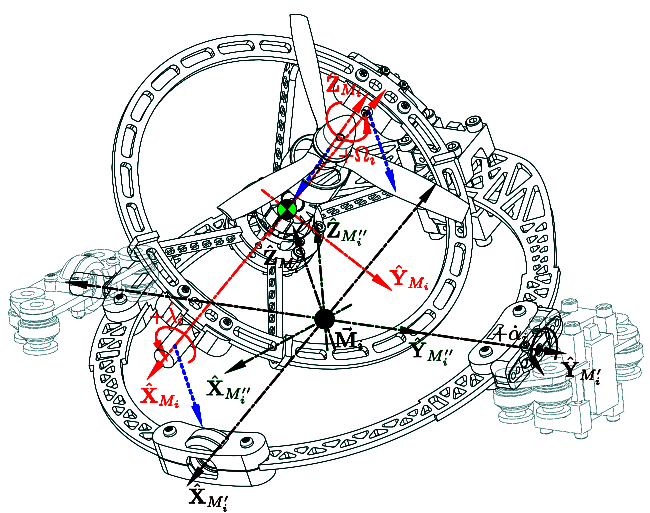
\includegraphics[width=0.85\textwidth]{figs/response-middle}
\vspace{-12pt}
\caption{Exploded middle ring inertial bodies for $\vec{\tau}_{\alpha}(\lambda_i,\alpha_i)$}
\label{fig:response-middle}
\vspace{-16pt}
\end{figure}
\par
Similarly for the middle ring frame $\mathcal{F}^{M_i'}$ relative to the intermediary frame $\mathcal{F}^{M_i''}$ the only relative path variable is $\vec{\mathbf{v}}(t)=\begin{bmatrix}0 & \alpha_i & 0\end{bmatrix}^T$. The entire motor module's structure consists of three separate rotating bodies each with their own relative angular velocities; the \emph{rotor} assembly, \emph{inner} and \emph{middle} ring structures; exploded in Fig:\ref{fig:response-middle}. 
\par
Applying the same process to evaluate the $ \alpha_i$ servo's response, the middle ring assembly Lagrangian $\mathcal{L}_{m/p}$ is constructed but with respect to the intermediary frame $\mathcal{F}^{M_i''}$. First transforming the inertias; the rotor assembly, further rotated by $\alpha_i$ about its $\hat{Y}_{M_i'}$ axis, has an inertia aligned with axes in $\mathcal{F}^{M_i''}$:
\begin{subequations}
\begin{equation}\label{eq:rotor-inertia-mid}
J_r''=R_y(\alpha_i)\big(J_r'\big)R_y^{-1}(\alpha_i)=R_y(\alpha_i)R_x(\lambda_i)\big(J_r\big)R_x^{-1}(\lambda_i)R_y^{-1}(\alpha_i)
\end{equation}
Which has a time derivative $\dot{J}_r''$:
\begin{equation}\label{eq:rotor-inertia-rate}
\dot{J}_r''=R_y(\alpha_i)\big(\dot{J}_r'\big)R_y^{-1}(\alpha_i)+[\dot{\vec{\alpha}}_i]_\times R_y(\alpha_i)\big(J_r'\big)R_y^{-1}(\alpha_i)-R_y(\alpha_i)\big(J_r'\big)[\dot{\vec{\alpha}}_i]_\times R_y^{-1}(\alpha_i)
\end{equation}
\end{subequations}
The inner ring structure has an inertia, still \emph{without} including the rotor assembly, aligned with $\mathcal{F}^{M_i''}$:
\begin{subequations}
\begin{equation}\label{eq:inner-inertia-mid}
J_{ir}''=R_y(\alpha_i)\big(J_{ir}'\big)R_y^{-1}(\alpha_i)=R_y(\alpha_i)R_x(\lambda_i)\big(J_{ir}\big)R_x^{-1}(\lambda_i)R_y^{-1}(\alpha_i)
\end{equation} 
Similarly, the time derivative $\dot{J}_{ir}''$ is:
\begin{equation}\label{eq:inner-inertia-rate}
\dot{J}_{ir}''=R_y(\alpha_i)\big(\dot{J}_{ir}'\big)R_y^{-1}(\alpha_i)+[\dot{\vec{\alpha_i}}\hspace{2pt}]_\times R_y(\alpha_i)\big(J_{ir}'\big)R_y^{-1}(\alpha_i)-R_y(\alpha_i)\big(J_{ir}'\big)[\dot{\vec{\alpha}}\hspace{2pt}]_\times R_y^{-1}(\alpha_i)
\end{equation}
\end{subequations}
Finally the middle ring structure's inertia from Eq:\ref{eq:inertia.middle.a}, with neither the rotor's nor the inner ring's contributions:
\begin{subequations}
\begin{equation}\label{eq:middle-inertia-mid}
J_m'=R_y(\alpha_i)\big(J_\text{m}\big)R_y^{-1}(\alpha_i)
\end{equation}
Which, when using the collective motor module inertia $J_p$ from Eq:\ref{eq:inertia.middle.b}, expands to:
\begin{equation}
J_m'=R_y(\alpha_i)\big(J_\text{p}\big)R_y^{-1}(\alpha_i)-R_y(\alpha_i)R_x(\lambda_i)\big(J_\text{n}\big)R_x^{-1}(\lambda_i)R_y^{-1}(\alpha_i)
\end{equation}
\vspace{-18pt}
\begin{equation}\label{eq:middle-inertia-relation}
=J_\text{p}'-J_{n}''=J_\text{p}'-\big(J_{ir}''+J_{r}''\big)
\end{equation}
Which has a time derivative purely as a result of $\dot{\alpha}$:
\begin{equation}
\dot{J}_m'=[\dot{\vec{\alpha}}_i]_\times R_y(\alpha_i)\big(J_m\big)R_y^{-1}(\alpha_i)-R_y(\alpha_i)\big(J_m\big)[\dot{\vec{\alpha}}_i]_\times R_y^{-1}(\alpha_i)
\end{equation}
However; that derivative $\dot{J}_m'$, using $\dot{J}_{r}''$ and $\dot{J}_{ir}''$ from Eq:\ref{eq:rotor-inertia-rate} and Eq:\ref{eq:inner-inertia-rate} respectively, expands to:
\begin{equation}\label{eq:middle-inertia-rate}
\dot{J}_m'=[\dot{\vec{\alpha}}_i]_\times R_y(\alpha_i)\big(J_p\big)R_y^{-1}(\alpha_i)-R_y(\alpha_i)\big(J_p\big)[\dot{\vec{\alpha}}_i]_\times R_y^{-1}(\alpha_i)-(\dot{J}_{ir}''+\dot{J}_{r}'')
\end{equation}
\end{subequations}
Note that introducing the relations of Eq:\ref{eq:middle-inertia-relation} and Eq:\ref{eq:middle-inertia-rate} to the collective body inertia $J_p$ is to simplify the subsequent equations. Each body then has its own relative angular velocity with respect to the intermediate frame $\mathcal{F}^{M_i''}$. For the rotor; $\vec{\omega}_{r/p}$ is the relative angular velocity of that assembly from the motor $\Omega_i$ and both inner and middle servo rates $\dot{\lambda}_i$ and $\dot{\alpha}_i$:
\begin{subequations}\label{eq:rotor-relative}
\begin{equation}
\vec{\omega}_{r/p}\triangleq R_y(\alpha_i)R_x(\lambda_i)\vec{\Omega}_i+R_y(\alpha_i)\dot{\vec{\lambda}}_i+\dot{\vec{\alpha}}_i~~~~\in\mathcal{F}^{M_i''}
\end{equation}
\vspace{-12pt}
\begin{equation}
\therefore \vec{\omega}_{r/p}=\vec{\Omega}_i\text{}\hspace{-2pt}''+\dot{\vec{\lambda}}_i\text{}\hspace{-2pt}'+\dot{\vec{\alpha}}_i
\end{equation}
\end{subequations}
Where $\vec{\Omega}_i''$ and $\dot{\vec{\lambda}}_i'$ are respectively propeller and inner servo velocities transformed to the frame $\mathcal{F}^{M_i''}$. Next, the inner ring has an angular velocity $\vec{\omega}_{n/p}$ relative to the intermediate frame $\mathcal{F}^{M_i''}$ from the two servo rates $\dot{\lambda}_i$ and $\dot{\alpha}_i$:
\begin{equation}\label{eq:inner-relative}
\vec{\omega}_{n/p}\triangleq R_y(\alpha_i)\dot{\vec{\lambda}}_i+\dot{\vec{\alpha}}_i=\dot{\vec{\lambda}}_i\text{}\hspace{-2pt}'+\dot{\vec{\alpha}}_i~~~~\in\mathcal{F}^{M_i''}
\end{equation}
Lastly the middle ring body has an angular velocity $\vec{\omega}_{m/p}$ relative to the intermediary frame only as a result of the middle ring's servo velocity $\dot{\alpha}_i$:
\begin{equation}\label{eq:middle-relative}
\vec{\omega}_{m/p}\triangleq=\dot{\vec{\alpha}}_i~~~~\in\mathcal{F}^{M_i''}
\end{equation}
Using the relative path coordinate $\vec{\mathbf{v}}(t)$, the Lagrangian $\mathcal{L}_{m/p}$ can be constructed for the complete motor module relative to the intermediate frame $\mathcal{F}^{M_i''}$ with kinetic energies of the rotor assembly, inner and middle ring structures respectively:
\begin{equation}\label{eq:alpha-lagrange}
\mathcal{L}_{m/p}=\frac{1}{2}\vec{\omega}_{r/p}^{\hspace{2pt}T}\big(J_{r}''\big)\vec{\omega}_{r/p}+\frac{1}{2}\vec{\omega}_{n/p}^{\hspace{2pt}T}\big(J_{ir}''\big)\vec{\omega}_{n/p}+\frac{1}{2}\vec{\omega}_{m/p}^{\hspace{2pt}T}\big(J_{m}'\big)\vec{\omega}_{m/p}
\end{equation}
Where Eq:\ref{eq:alpha-lagrange} again does not include any potential energy gravitational contributions because such quantities are incorporated in Eq:\ref{eq:grav-torque}. The middle ring's Lagrangian $\mathcal{L}_{m/p}$ from Eq:\ref{eq:alpha-lagrange} therefore expands to:
\begin{multline}\label{eq:alpha-lagrange-two}
\mathcal{L}_{m/p}=\frac{1}{2}\Big[R_y(\alpha_i)R_x(\lambda_i)\vec{\Omega}_i+R_y(\alpha_i)\dot{\vec{\lambda}}_i+\dot{\vec{\alpha}}_i\Big]^T\big(J_r''\big)\Big[R_y(\alpha_i)R_x(\lambda_i)\vec{\Omega}_i+Ry(\alpha_i)\dot{\vec{\lambda}}_i+\dot{\vec{\alpha}}_i\Big]\\
+\frac{1}{2}\Big[R_y(\alpha_i)\dot{\vec{\lambda}}_i+\dot{\vec{\alpha}}_i\Big]^T\big(J_{ir}''\big)\Big[R_y(\alpha_i)\dot{\vec{\lambda}}_i+\dot{\vec{\alpha}}_i\Big]
+\frac{1}{2}\dot{\vec{\alpha}}_i^{\hspace{2pt}T}\big(J_m'\big)\dot{\vec{\alpha}}_i
\end{multline}
Extending the path coordinate partial derivative reduction from Eq:\ref{eq:euler-lagrange-inner-partial}, the Euler-Lagrange formulation for the middle ring then simplifies with the partial derivative $\partial\mathcal{L}_{m/p}/\partial\vec{\mathbf{v}}=0$. So the generalized forces (torques) $\vec{\mathbf{V}}(\lambda_i,\alpha_i)$ acting on the middle ring are:
\begin{equation}
\vec{\mathbf{V}}(\lambda_i,\alpha_i)=\frac{d}{dt}\Bigg(\frac{\partial\mathcal{L}_{m/p}}{\partial\dot{\vec{\mathbf{v}}}}\Bigg)-\frac{\partial\mathcal{L}_{m/p}}{\partial\vec{\mathbf{v}}}=\frac{d}{dt}\Bigg(\frac{\partial\mathcal{L}_{m/p}}{\partial\dot{\vec{\mathbf{v}}}}\Bigg)~~~~\in\mathcal{F}^{M_i''}
\end{equation}
Finding the partial derivative of $\mathcal{L}_{m/p}$ in Eq:\ref{eq:alpha-lagrange-two} with respect to the middle ring servo's relative path coordinate rate $\dot{\vec{\mathbf{v}}}$ yields:
\begin{subequations}
\begin{equation}
\frac{\partial\mathcal{L}_{m/p}}{\partial\dot{\vec{\mathbf{v}}}}=\big(J_r''\big)\Big[\vec{\Omega}_i\hspace{-2pt}''+\dot{\vec{\lambda}}_i\hspace{-2pt}'+\dot{\vec{\alpha}}_i\Big]+\big(J_{ir}''\big)\Big[\dot{\vec{\lambda}}_i\hspace{-2pt}'+\dot{\vec{\alpha}}_i\Big]+\big(J_m'\big)\dot{\vec{\alpha}}_i
\end{equation}
Which with relative rotor, inner and middle ring angular velocity definitions from Eq:\ref{eq:rotor-relative},\ref{eq:inner-relative} and \ref{eq:middle-relative} respectively; expands to:
\begin{equation}\label{eq:3.86b}
\frac{\partial\mathcal{L}_{m/p}}{\partial\dot{\vec{\mathbf{v}}}}=\big(J_r''\big)\Big[R_y(\alpha_i)R_x(\lambda_i)\vec{\Omega}_i+R_y(\alpha_i)\dot{\vec{\lambda}}_i+\dot{\vec{\alpha}}_i\Big]+\big(J_{ir}''\big)\Big[R_y(\alpha_i)\dot{\vec{\lambda}}_i+\dot{\vec{\alpha}}_i\Big]+\big(J_m'\big)\dot{\vec{\alpha}}_i
\end{equation}
Taking the time derivative of Eq:\ref{eq:3.86b} and using inertia rates for rotor, inner and middle rings each defined in Eq:\ref{eq:rotor-inertia-rate},\ref{eq:inner-inertia-rate} and \ref{eq:middle-inertia-rate} respectively; split into product ruled derivative components gives:
\begin{multline}\label{eq:alpha-lagrange-deriv}
\vec{\mathbf{V}}(\lambda_i,\alpha_i)=\frac{d}{dt}\Bigg(\frac{\partial \mathcal{L}_{m/p}}{\partial\dot{\vec{\mathbf{v}}}}\Bigg)=\Big[\big(\dot{J}_r''\big)(\vec{\Omega}_i\hspace{-2pt}''+\dot{\vec{\lambda}}_i\hspace{-2pt}'+\dot{\vec{\alpha}}_i)\Big]
\\
+\Big[\big(J_r''\big)\dot{\vec{\Omega}}_i\hspace{-2pt}''+\vec{\omega}_{n/p}\times\big(J_r''\big)\vec{\Omega}_i\hspace{-2pt}''+\big(J_r''\big)\ddot{\vec{\lambda}}_i\hspace{-2pt}'+\vec{\omega}_{n/p}\times \big(J_r''\big)\dot{\vec{\lambda}}_i\hspace{-2pt}'+\big(J_r''\big)\ddot{\vec{\alpha}}_i+\vec{\omega}_{m/p}\times \big(J_r''\big)\dot{\vec{\alpha}}_i\Big]
\\
+\Big[\big(\dot{J}_{ir}''\big)(\dot{\vec{\lambda}}_i\hspace{-2pt}'+\dot{\vec{\alpha}}_i)\Big]
+\Big[\big(J_{ir}''\big)\ddot{\vec{\lambda}}_i\hspace{-2pt}'+\vec{\omega}_{n/p}\times\big(J_{ir}''\big)\dot{\vec{\lambda}}_i\hspace{-2pt}'+\big(J_{ir}''\big)\ddot{\vec{\alpha}}_i+\vec{\omega}_{m/p}\times\big(J_{ir}''\big)\dot{\vec{\alpha}}_i\Big]
\\
+\Big[\big(\dot{J}_m'\big)\dot{\vec{\alpha}}_i\Big] +\Big[\big(J_m'\big)\ddot{\vec{\alpha}}_i+\vec{\omega}_{m/p}\times\big(J_m'\big)\dot{\vec{\alpha}}_i\Big]
\end{multline}
With relative frame angular velocities; $\vec{\omega}_{n/p}$ of the inner ring relative to the intermediate frame, and $\vec{\omega}_{m/p}$ of the middle ring relative to the intermediate frame. Both are defined respectively:
\begin{equation}
\vec{\omega}_{n/p}\triangleq R_y(\alpha_i)\dot{\vec{\lambda}}_i+\dot{\vec{\alpha}}_i=\dot{\vec{\lambda}}_i\hspace{-2pt}'+\dot{\vec{\alpha}}_i~~~~\in\mathcal{F}^{M_i''}
\end{equation}
\vspace{-16pt}
\begin{equation}
\vec{\omega}_{m/p}\triangleq\dot{\vec{\alpha}}_i~~~~\in\mathcal{F}^{M_i''}
\end{equation}
\par
Eq:\ref{eq:alpha-lagrange-deriv} is an ominous and decidedly complicated result to expand and make sense of. However it can be simplified; recognizing that generalized torques for the middle ring in Eq:\ref{eq:alpha-lagrange-deriv} contain inner ring kinetic energies already introduced in Eq:\ref{eq:torque-induced-inner}, but transformed to the frame $\mathcal{F}^{M_i''}$. 
\par
After some mathematics, Eq:\ref{eq:alpha-lagrange-deriv} can be simplified into two parts; responses pertinent to $\Delta\alpha_i$ and the transformed inner ring generalized response $R_y(\alpha_i)\vec{\tau}_\lambda(\lambda_i)$:
\begin{multline}\label{eq:3.63f}
\vec{\mathbf{V}}(\lambda_i,\alpha_i)=R_y(\alpha_i)\frac{d}{dt}\bigg(\frac{\partial\mathcal{L}_{n/m}}{\partial\dot{\vec{\mathbf{u}}}}\bigg)+\Big(R_y(\alpha_i)\big(\dot{J}_r'\big)R_y^{-1}(\alpha_i)\Big)\dot{\vec{\alpha}}_i+\Big(\dot{J}_r''-R_y(\alpha_i)\big(\dot{J}_r'\big)R_y^{-1}(\alpha_i)\Big)\big(\vec{\Omega}_i''+\dot{\vec{\lambda}}_i'+\dot{\vec{\alpha}}_i\big)
\\
+\big(J_r''\big)\ddot{\vec{\alpha}}_i+\dot{\vec{\alpha}}_i\times\big(J_r''\big)\Big(\vec{\Omega}_i''+\dot{\vec{\lambda}}_i'+\dot{\vec{\alpha}}_i\Big)+\Big(R_y(\alpha_i)\big(\dot{J}_{ir}'\big)R_y^{-1}(\alpha_i)\Big)\dot{\vec{\alpha}}_i+\Big(\dot{J}_{ir}''-R_y(\alpha_i)\big(\dot{J}_{ir}'\big)R_y^{-1}(\alpha_i)\Big)\big(\dot{\vec{\lambda}}_i'+\dot{\vec{\alpha}}_i\big)
\\
+\big(J_{ir}''\big)\ddot{\vec{\alpha}}_i+\dot{\vec{\alpha}}_i\times \big(J_{ir}''\big)\Big(\dot{\vec{\lambda}}_i\hspace{-2pt}'+\dot{\vec{\alpha}}_i\Big)+\big(\dot{J}_m'\big)\dot{\vec{\alpha}}_i+\big(J_m'\big)\ddot{\vec{\alpha}}_i+\dot{\vec{\alpha}}_i\times \big(J_m'\big)\dot{\vec{\alpha}}_i
\end{multline}
Paying special attention to differentiate $\dot{J}_{r}''$ and $\dot{J}_{ir}''$ from Eq:\ref{eq:rotor-inertia-rate} and Eq:\ref{eq:inner-inertia-rate} respectively with $R_y(\alpha_i)\big(\dot{J}_r'\big)R_y^{-1}(\alpha_i)$ and $R_y(\alpha_i)\big(\dot{J}_{ir}'\big)R_y^{-1}(\alpha_i)$. Where the latter two terms are inertia rates of change from Eq:\ref{eq:rotor-deriv} and Eq:\ref{eq:inner-deriv}, but transformed to the frame $\mathcal{F}^{M_i''}$. 
\par
Generalized torques in Eq:\ref{eq:3.63f} can be further simplified by introducing combined inertial bodies $J_n=J_r+J_{ir}$ for the \emph{entire} inner ring from Eq:\ref{eq:inertia.inner} and $J_p=J_m+R_x(\lambda_i)\big(J_n\big)R_x^{-1}(\lambda_i)$ for the \emph{entire} motor module's inertia from Eq:\ref{eq:inertia.middle.b}. Using $J_p'=R_y(\alpha_i)\big(J_p\big)R_y^{-1}(\alpha_i)$ and $J_n'=R_y(\alpha_i)\big(J_n\big)R_y^{-1}(\alpha_i)$ for the net module's inertia and the entire inner ring inertia both respectively aligned with the frame $\mathcal{F}^{M_i''}$:
\begin{multline}\label{eq:3.86g}
\vec{\mathbf{V}}(\lambda_i,\alpha_i)=R_y(\alpha_i)\vec{\mathbf{U}}(\lambda_i)+\Big(R_y(\alpha_i)\big(\dot{J}_n'\big)R_y(\alpha_i)\Big)\dot{\vec{\alpha}}_i+ \Big(\dot{J}_p'-R_y(\alpha_i)\big(\dot{J}_p\big)R_y^{-1}(\alpha_i)\Big)\dot{\vec{\alpha}}_i
\\
+\Big(\dot{J}_n''-R_y(\alpha_i)\big(\dot{J}_n'\big)R_y^{-1}(\alpha_i)\Big)\dot{\vec{\lambda}}'+\Big(\dot{J}_r''-R_y(\alpha_i)\big(\dot{J}_r'\big)R_y^{-1}(\alpha_i)\Big)\vec{\Omega}_i''
\\
+J_p'\ddot{\vec{\alpha}}_i+\dot{\vec{\alpha}}_i\times\Big(\big(J_p'\big)\dot{\vec{\alpha}}+\big(J_n''\big)\dot{\vec{\lambda}}_i'+\big(J_r''\big)\vec{\Omega}_i''\Big)
\end{multline}
\end{subequations}
Noting that $\dot{J}_p = \dot{J}_r'+\dot{J}_{ir}'+\dot{J}_m$ and that $\dot{J}_m=0$, it follows that $\dot{J}_p =\dot{J}_n'$. Isolating the servo's torque response from $\Delta\alpha_i$, and again grouping inertial bodies with shared angular velocities together. The \emph{inertia rates}, second order \emph{inertia} and first order \emph{gyroscopic} responses are then:
\begin{multline} \label{eq:torque-induced-middle}
\vec{\tau}_\alpha(\lambda_i,\alpha_i)=\underbrace{\big(\dot{J}_p'\big)\dot{\vec{\alpha}}_i+\Big(\dot{J}_n''-R_y(\alpha)\big(\dot{J}_n'\big)R_y^{-1}(\alpha)\Big)\dot{\vec{\lambda}}_i'+\Big(\dot{J}_r''-R_y(\alpha)\big(\dot{J}_r'\big)R_y^{-1}(\alpha)\Big)\vec{\Omega}_i''}_{\text{Inertia rates}}
\\
+\underbrace{\big(J_\text{p}'\big)\ddot{\vec{\alpha}}_i}_{\text{Inertia}}+\underbrace{\dot{\vec{\alpha}}_i\times \Big(\big(J_p'\big)\dot{\vec{\alpha}}_i+\big(J_n''\big)\dot{\vec{\lambda}}_i\hspace{-2pt}'+\big(J_r''\big)\vec{\Omega}_i\hspace{-2pt}''\Big)}_{\text{Gyroscopic}}~~~~\in\mathcal{F}^{M_i''}
\end{multline}
It is important to stress that the servo's response $\vec{\tau}_\alpha(\lambda_i,\alpha_i)$ is \underline{\emph{\textbf{not}}} the same as the generalized torque $\vec{\mathbf{V}}(\lambda_i,\alpha_i)$ described in Eq:\ref{eq:3.86g}. The latter contains terms for the inner ring's servo response. Careful inspection could have yielded the inertia and gyroscopic components of both Eq:\ref{eq:torque-induced-inner} and Eq:\ref{eq:torque-induced-middle}, however the effect of inertia time derivatives on the torque system is a far less obvious result. Each servo's respective induced torques, $\vec{\tau}_\lambda(\lambda_i)$ and $\vec{\tau}_\alpha(\lambda_i,\alpha_i)$, occur in sequential gimbal-like frames. The opposing negative responses to induced relative rotations effect the angular state dynamics in Eq:\ref{eq:states.d}, and must be transformed to the common body frame:
\begin{subequations}\label{eq:torque-response}
\begin{equation}
\vec{\tau}_Q(u)=-\sum_{i=1}^4 \Big(R_z(\sigma_i)R_y(\alpha_i)\vec{\tau}_{\lambda}(\lambda_i)+R_z(\sigma_i)\vec{\tau}_{\alpha}(\alpha_i,\lambda_i)\Big)~~~~\in\mathcal{F}^b
\end{equation}
\vspace{-12pt}
\begin{equation}
=-\sum_{i=1}^4R_z(\sigma_i)\vec{\mathbf{V}}(\lambda_i,\alpha_i)
\end{equation}
\end{subequations}
The final non-trivial torque term associated with the multibody motion which must be accounted for is the entire system's response to motion relative to the inertial frame $\mathcal{F}^{I}$. Specifically considering the responses relative rotations $\Delta\lambda_i$ and $\Delta\alpha_i$ have to the net angular velocity of the entire multibody system $\vec{\omega}_b$. Such responses are an extension of the fundamental rigid 6-DOF differential equation for angular motion, reiterated from Eq:\ref{eq:angular-multibody}:
\begin{equation}
\dot{\vec{\omega}}_b=\big(J_b^{-1}\big)\Big(-\vec{\omega}_b\times\big(J_b\big)\vec{\omega}_b+\vec{\tau}_{\mu}\Big)~~~~\in\mathcal{F}^b
\end{equation}
Before continuing with a Lagrangian formulation applied to the entire multibody vehicle; it is worth first establishing an axiom to add some clarity to the steps which follow. Consider the hypothetical rotating, non-Newtonian 2-D system illustrated in Fig:\ref{fig:lemma-1}. 
\begin{figure}[htbp]
\centering
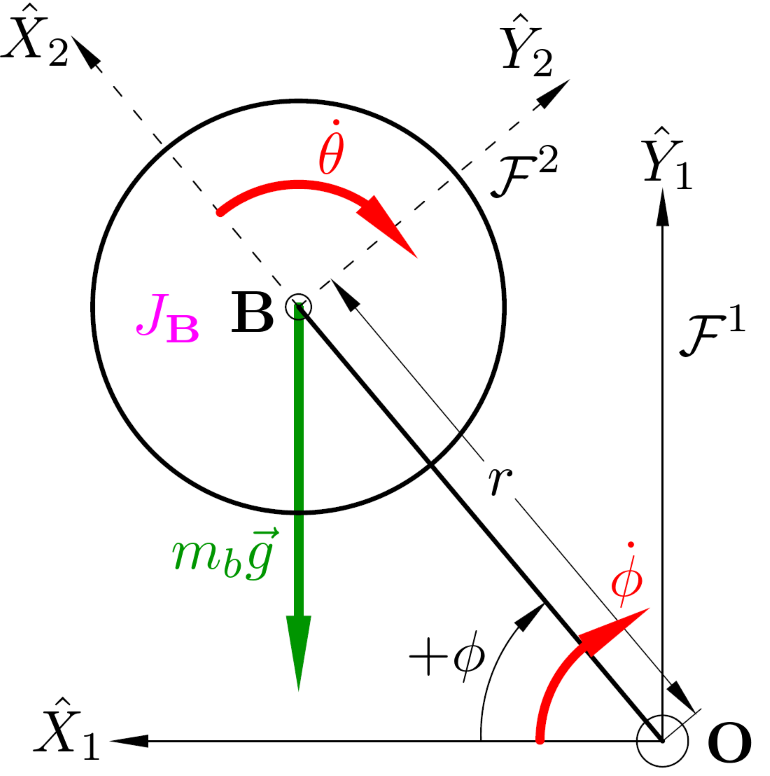
\includegraphics[width=0.43\textwidth]{figs/lemma-1}
\vspace{-6pt}
\caption{Rotating system}
\label{fig:lemma-1}
\vspace{-18pt}
\end{figure} 
\par
A massless rod of length $r$ connects some rotational body, with a mass $m_b$, at point $\mathbf{B}$ to a center pivot point $\mathbf{O}$. The principle frame $\mathcal{F}^{1}$ has axes $\hat{X}_1$ and $\hat{Y}_1$ as illustrated. The arm has a rotational velocity $\dot{\phi}$ relative to $\hat{X}_1$ in $\mathcal{F}^{1}$, applied by some ``motor". Attached to the end of the rod is a secondary frame $\mathcal{F}^2$ with an $\hat{X}_2$ axis, co-linear to the rod and a perpendicular $\hat{Y}_2$. The rotational body, centered at point $\mathbf{B}$, has a rotational inertia $J_\mathbf{B}$ about the point (or axis) at $\mathbf{B}$. That rotating body has a rotational velocity $\dot{\theta}$ from another ``motor" relative to $\mathcal{F}^2$. The question is then how to find the net torque applied to the system about point $\mathbf{O}$ in terms of angular velocities $\dot{\phi}$ and $\dot{\theta}$ and their derivatives (or accelerations)?
\begin{figure}[htbp]
\centering
\begin{subfigure}{0.43\textwidth}
\centering
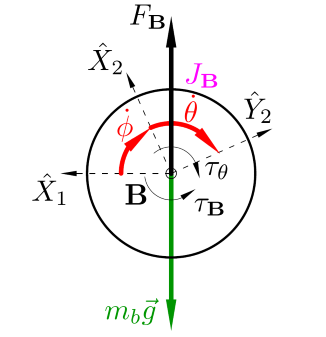
\includegraphics[width=\textwidth]{figs/lemma-a}
\caption{Rotational body}
\label{fig:lemma-a}
\end{subfigure}
\begin{subfigure}{0.43\textwidth}
\centering
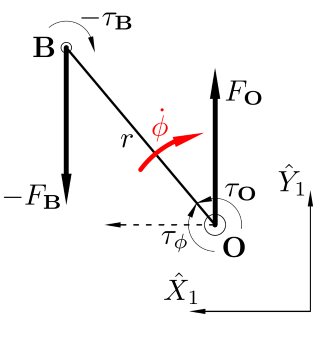
\includegraphics[width=\textwidth]{figs/lemma-b}
\caption{Massless rod}
\label{fig:lemma-b}
\end{subfigure}
\caption{Free-body diagram for rotational system}
\label{fig:lemma}
\vspace{-12pt}
\end{figure}
\par
Isolated free body diagrams for each body under consideration are illustrated in Fig:\ref{fig:lemma}. Considering the rotational body only (Fig:\ref{fig:lemma-a}) the torque acting about point $\mathbf{B}$ is simply an inertia response to combined angular accelerations of $\ddot{\theta}$ and $\ddot{\alpha}$:
\begin{equation}
\tau_\mathbf{B}=-\tau_\theta=-J_\mathbf{B}(\ddot{\theta}+\ddot{\phi})~~~~\in\mathcal{F}^2
\end{equation}
The net force acting on the rotational body is purely the gravitational force acting through point $\mathbf{B}$ as a result of the mass $m_b$ and some gravitational force vector $\vec{g}\in\mathcal{F}^2$:
\begin{equation}
F_\mathbf{B}=-G=-m_b\vec{g}~~~~\in\mathcal{F}^2
\end{equation}
That torque and force pair, $F_\mathbf{B}$ and $\tau_\mathbf{B}$, are transferred to frame $\mathcal{F}^1$ through the massless rod connecting point $\mathbf{B}$ to $\mathbf{O}$, Fig:\ref{fig:lemma-b}. The net torque acting around point $\mathbf{O}$ is then comprised of three components; inferred torque from $\tau_\mathbf{B}$, a torque arm from force $F_\mathbf{B}$ and an inertia torque response to the effective ``point-mass" at point $\mathbf{B}$ relative to $\mathbf{O}$:
\begin{equation}
\tau_\mathbf{O}=-\tau_\phi=-\tau_\mathbf{B}-F_\mathbf{B}r\cos{\phi}+m_br^2(\ddot{\phi})~~~~\in\mathcal{F}^1
\end{equation}
\par
The net response force acting at point $\mathbf{O}$, $F_\mathbf{O}$, is of no consequence to the calculation of net torques. The ``motor" applies a torque $\tau_\phi$ to the rod to induce some angular acceleration $\ddot{\phi}$ on the whole system. Opposed to that angular acceleration is the torque $\tau_\mathbf{O}$ which acts against that rotation. The torque $\tau_\phi$ acting on the system can then be simplified:
\begin{equation}
\tau_\phi=J_\mathbf{B}(\ddot{\theta}+\ddot{\phi})+m_br^2(\ddot{\phi})-m_b\vec{g}\hspace{1pt}r\cos\phi~~~~\in\mathcal{F}^1
\end{equation}
That result would not be as obvious when inferred from an energy equation. The equivalent Lagrangian for net kinetic and potential energy of the system, $T$ and $U$ respectively relative to $\mathcal{F}^1$, would be:
\begin{subequations}
\begin{equation}
\mathcal{L}=T(\theta,\phi)-U(\theta,\phi)
\end{equation}
\vspace{-14pt}
\begin{equation}\label{eq:lemma-lagrange}
\mathcal{L}=\frac{1}{2}\vec{\omega}_\mathbf{B}\hspace{-2pt}^T\big(J_\mathbf{B}\big)\vec{\omega}_\mathbf{B}+\frac{1}{2}\vec{\omega}_\mathbf{O}\hspace{-2pt}^T\big(J_\mathbf{O}\big)\vec{\omega}_\mathbf{O}-m_b\vec{g}r\sin{\phi}
\end{equation}
Where $\vec{\omega}_\mathbf{B}$ and $\vec{\omega}_\mathbf{O}$ are net angular velocities of the rotational body and massless connection rod respectively. The important thing to consider is that $J_\mathbf{O}$, the net rotational inertia about the point $\mathbf{O}$, is simply the point mass inertia $m_br^2$ and \underline{\textbf{not}} the expected parallel axis theorem $J_\mathbf{O}\not=J_\mathbf{B}'=J_\mathbf{B}+m_br^2$. Expanding Eq:\ref{eq:lemma-lagrange} and applying the Euler-Lagrange formulation, using a partial derivative with respect to the path coordinate $\phi$ to produce the generalized torque $\tau_\phi$ acting on the system:
\begin{equation}
\mathcal{L}=\frac{1}{2}\Big(\dot{\theta}+\dot{\phi}\Big)^T\big(J_\mathbf{B}\big)\Big(\dot{\theta}+\dot{\phi}\Big)+\Big(\dot{\phi}\Big)\big(m_br^2\big)\Big(\dot{\phi}\Big)-m_b(-g)r\sin\phi
\end{equation}
\vspace{-14pt}
\begin{equation}
\text{Genealized forces}=\frac{d}{dt}\bigg(\frac{\partial\mathcal{L}}{\partial\dot{\phi}}\bigg)-\frac{\partial\mathcal{L}}{\partial\phi}=\vec{\tau}_\phi
\end{equation}
\vspace{-8pt}
\begin{equation}
=\frac{d}{dt}\bigg(\big(J_\mathbf{B}\big)\Big(\dot{\theta}+\dot{\phi}\Big)+\big(m_br^2\big)\Big(\dot{\phi}\Big)\bigg)-m_bgr\cos\phi
\end{equation}
\vspace{-8pt}
\begin{equation}
\therefore\tau_\phi=J_\mathbf{B}(\ddot{\theta}+\ddot{\phi})+m_br^2(\ddot{\phi})-m_bgr\cos\phi
\end{equation}
\vspace{-14pt}
\begin{equation}\label{eq:lemma-torque}
=J_\mathbf{B}\ddot{\theta}+J_\mathbf{B}'\ddot{\phi}+\tau_g
\end{equation}
\end{subequations}
Where $J_b'$ is the \underline{\textbf{parallel axis inertia}} and $\tau_g$ is the gravitational torque arm contribution. The above then leads to the claim asserted from the system described in Fig:\ref{fig:lemma-1}:
\begin{axiom}\label{lem:1}
A torque response opposed to angular acceleration of a doubly rotating body can be found as the contribution of the principle rotational inertia about the first axis of rotation with \underline{only} the first rotational acceleration and a parallel axis inertia about the second rotational axis with the second, independent rotational acceleration.
\\
(The same torque can be found as the inertial opposition to net angular acceleration, the sum of both rotations, about the first axis and a point mass inertia opposed to the second rotation about its respective axis.)
\end{axiom}
Returning to the net multibody system and separating the motor module from the entire body structure first (exploded bodies for \emph{motor module 1} in Fig:\ref{fig:response-body}). Considering only the additional contribution the angular velocity $\vec{\omega}_b$ has on a single motor module and later introducing the entire combined system; the Lagrangian derivation for motion relative to the inertial frame then follows.
\par
\begin{figure}[htbp]
\vspace{-12pt}
\centering
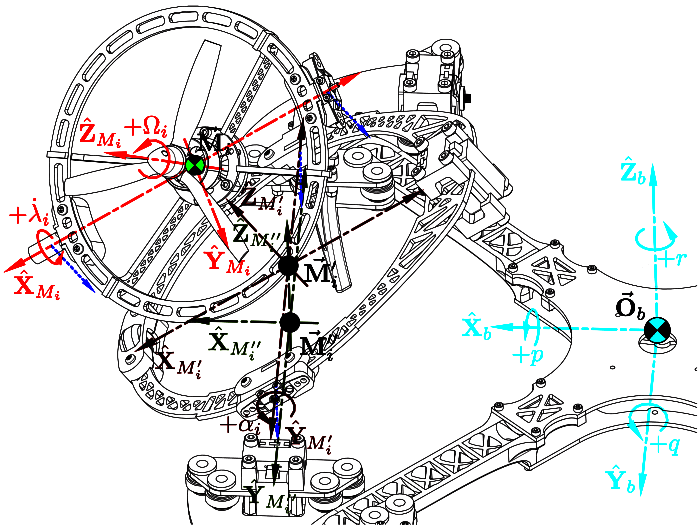
\includegraphics[width=0.9\textwidth]{figs/response-body}
\vspace{-8pt}
\caption{Exploded motor module inertial bodies for $\vec{\omega}_b$ response}
\label{fig:response-body}
\vspace{-18pt}
\end{figure}
The relative $\hat{Z}_{M_i''}$ rotation by $\sigma_i$ is what differentiates the intermediate frame $\mathcal{F}^{M_i''}$ (used for calculations pertinent to Fig:\ref{fig:response-middle}) and the body frame $\mathcal{F}^b$. The familiar rotor assembly, inner and middle ring structure's inertias from Eq:\ref{eq:rotor-inertia-mid},\ref{eq:inner-inertia-mid} and \ref{eq:middle-inertia-mid} have respective counterparts aligned with $\mathcal{F}^b$:
\begin{subequations}\label{eq:module-inertia-body}
\begin{equation}
J_r'''=R_z(\sigma_i)\big(J_r''\big)R_z^{-1}(\sigma_i)=R_z(\sigma_i)R_y(\alpha_i)R_x(\lambda_i)\big(J_r\big)R_x^{-1}(\lambda_i)R_y^{-1}(\alpha_i)R_z^{-1}(\sigma_i)
\end{equation}
\vspace{-12pt}
\begin{equation}
J_{ir}'''=R_z(\sigma_i)\big(J_{ir}''\big)R_z^{-1}(\sigma_i)=R_z(\sigma_i)R_y(\alpha_i)R_x(\lambda_i)\big(J_{ir}\big)R_x^{-1}(\lambda_i)R_y^{-1}(\alpha_i)R_z^{-1}(\sigma_i)
\end{equation}
\vspace{-12pt}
\begin{equation}
J_m''=R_z(\sigma_i)\big(J_m'\big)R_z^{-1}(\sigma_i)=R_z(\sigma_i)R_y(\alpha_i)\big(J_m\big)R_y^{-1}(\alpha_i)R_z^{-1}(\sigma_i)
\end{equation}
\end{subequations}
Where $\sigma_i$ in Eq:\ref{eq:module-inertia-body} is the relative orthogonal $\hat{Z}_{M_i''}$ difference between frames $\mathcal{F}^{M_i''}$ and $\mathcal{F}^b$ defined before in Eq:\ref{eq:motor-module-rotation} and illustrated previously in Fig:\ref{fig:body-frame}. Because $\sigma_i$ is constant for each $i\in[1:4]$, inertia rates for each component of the motor module is simply the transformations of $\dot{J}_r''$,$\dot{J}_{ir}''$ and $\dot{J}_m'$ previously in Eq:\ref{eq:rotor-inertia-rate},\ref{eq:inner-inertia-rate} and \ref{eq:middle-inertia-rate}. Or more generally, for some inertia $J$ constant in $\mathcal{F}^{M_i''}$, that inertia's rate in $\mathcal{F}^b$ is:
\begin{subequations}
\begin{equation}
\frac{d}{dt}\Big(R_z(\sigma)\big(J\big)R_z^{-1}(\sigma)\Big)=0
\end{equation}
Dropping the $\sigma_i$ argument to indicate $R_z(\sigma)$ is a constant, the rotor, inner and middle inertia rates of change relative to the body frame $\mathcal{F}^b$ then follow respectively:
\begin{equation}\label{eq:body-rotor-rate}
\dot{J}_r'''=R_z\big(\dot{J}_r''\big)R_z^{-1}
\end{equation}
\vspace{-14pt}
\begin{equation}\label{eq:body-inner-rate}
\dot{J}_{ir}'''=R_z\big(\dot{J}_{ir}''\big)R_z^{-1}
\end{equation}
\vspace{-12pt}
\begin{equation}\label{eq:body-middle-rate}
\dot{J}_m''=R_z\big(\dot{J}_m'\big)R_z^{-1}
\end{equation}
\end{subequations}
Similarly, angular velocities for each separate body (rotor, inner and middle rings) in $\mathcal{F}^b$ but relative to the inertial frame $\mathcal{F}^I$ are then, first for the rotor:
\begin{subequations}\label{eq:body-rotor-angular}
\begin{equation}
\vec{\omega}_{r/I}=\vec{\Omega}_i'''+\dot{\vec{\lambda}}_i''+\dot{\vec{\alpha}}_i\text{}\hspace{-2pt}'+\vec{\omega}_{b/I}~~~~\in\mathcal{F}^b
\end{equation}
\vspace{-16pt}
\begin{equation}
=R_zR_y(\alpha_i)R_x(\lambda_i)\vec{\Omega}_i+R_zR_y(\alpha_i)\dot{\vec{\lambda}}_i+R_z\dot{\vec{\alpha}}_i+\vec{\omega}_b
\end{equation}
\end{subequations}
Extending that to the inner ring's rotational velocity:
\begin{subequations}\label{eq:body-inner-angular}
\begin{equation}
\vec{\omega}_{n/I}=\dot{\vec{\lambda}}_i''+\dot{\vec{\alpha}}_i\text{}\hspace{-2pt}'+\vec{\omega}_{b/I}~~~~\in\mathcal{F}^b
\end{equation}
\vspace{-16pt}
\begin{equation}
=R_zR_y(\alpha_i)\dot{\vec{\lambda}}_i+R_z\dot{\vec{\alpha}}_i+\vec{\omega}_{b/I}
\end{equation}
\end{subequations}
And lastly the middle ring structure has a relative angular rate:
\begin{subequations}\label{eq:body-middle-angular}
\begin{equation}
\vec{\omega}_{m/I}=\dot{\vec{\alpha}}_i\text{}\hspace{-2pt}'+\vec{\omega}_{b/I}~~~~\in\mathcal{F}^b
\end{equation}
\vspace{-16pt}
\begin{equation}
=R_z\dot{\vec{\alpha}}_i+\vec{\omega}_b
\end{equation}
\end{subequations}
Noting that Axiom:\ref{lem:1} and the parallel axis term in Eq:\ref{eq:lemma-torque} refer to the parallel axis difference between the \emph{center of mass} and the resultant rotational axis. The vector difference between the rotated center of mass for a motor module $\vec{C}_\text{p}\text{}\hspace{-2pt}''(\lambda_i,\alpha_i)$ and the body frame origin $\vec{\mathbf{O}}_b$ is defined:
\begin{subequations}
\begin{equation}
\vec{C}_\text{p}\text{}\hspace{-2pt}''(\lambda_i,\alpha_i)=\frac{m_\text{n}\vec{C}_\text{n}\text{}\hspace{-2pt}'''(\lambda_i,\alpha_i)+m_\text{m}\vec{C}_\text{m}\text{}\hspace{-2pt}''(\alpha_i)}{m_\text{p}}
\end{equation}
With $\vec{C}_\text{n}\text{}\hspace{-2pt}'''(\lambda_i,\alpha_i)$ and $\vec{C}_\text{m}\text{}\hspace{-2pt}''(\alpha_i)$ being rotated inner and middle ring centers of mass respectively from Eq:\ref{eq:body-net-inner.d} and Eq:\ref{eq:body-net-middle.d}:
\begin{equation}
\therefore \vec{C}_\text{p}\text{}\hspace{-2pt}''(\lambda_i,\alpha_i)=\frac{m_\text{n}R_zR_y(\alpha_i)R_x(\lambda_i)\vec{C}_\text{n}+m_\text{m}R_zR_y(\alpha_i)\vec{C}_\text{m}}{m_\text{n}+m_\text{n}}
\end{equation}
\par
\begin{figure}[hbtp]
\vspace{-10pt}
\centering
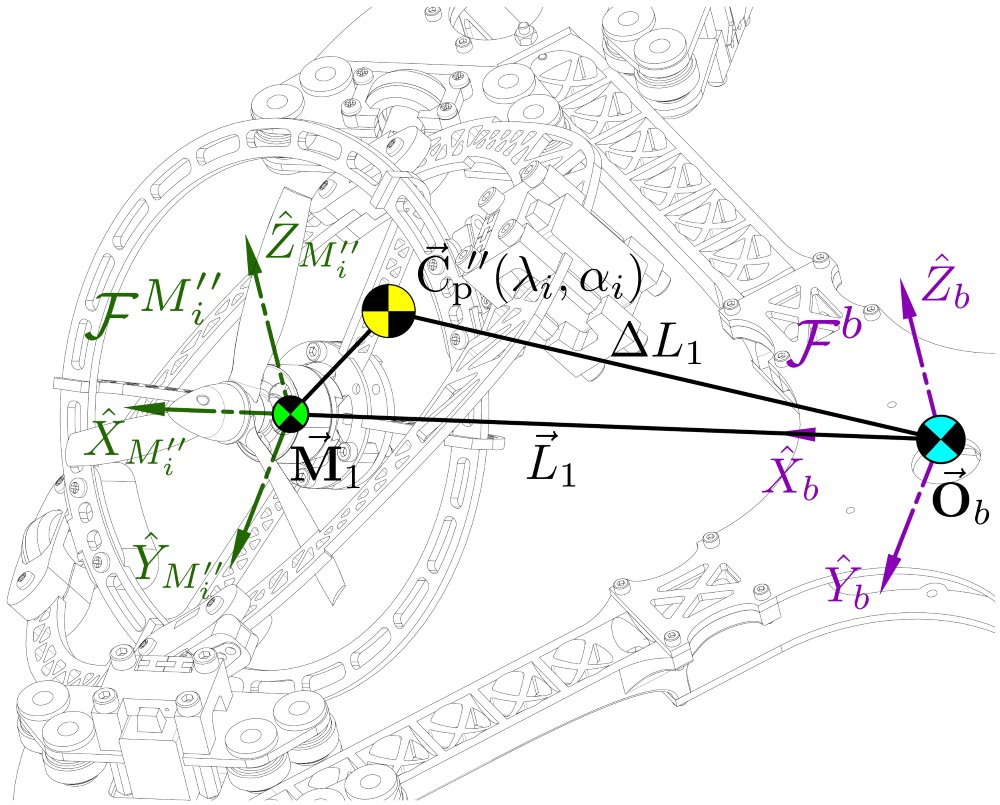
\includegraphics[width=0.9\textwidth]{figs/vector-diff}
\vspace{-6pt}
\caption{Illustration of rotated center of gravity $\vec{C}_\text{p}\text{}\hspace{-2pt}''(\lambda_i,\alpha_i)$}
\vspace{-6pt}
\label{fig:vector-diff}
\end{figure}
\par
This leads to the vector difference $\Delta \vec{L}_i$, with $L=196.15~\text{mm}$ illustrated for module 1 in Fig:\ref{fig:vector-diff}.
\begin{equation}
\Delta \vec{L}_i=\vec{L}_i+\vec{C}_\text{p}\text{}\hspace{-2pt}''(\lambda_i,\alpha_i)
\end{equation}
The time derivative of that module's moving center of gravity, $d/dt\big(\vec{C}_\text{p}\text{}\hspace{-2pt}''(\lambda_i,\alpha_i)\big)$ relative to the origin $\vec{\mathbf{O}}_b$, is:
\begin{equation}
\Delta \dot{\vec{L}}_i=\frac{d}{dt}\Big(\vec{C}_\text{p}\text{}\hspace{-2pt}''(\lambda_i,\alpha_i)\Big)
\end{equation}
\vspace{-14pt}
\begin{multline}
=\frac{1}{m_\text{p}}\Big(m_\text{n}\big(R_z\big([\dot{\vec{\alpha}}_i]_\times R_y(\alpha_i)R_x(\lambda_i)\vec{C}_\text{n}+R_y(\alpha_i)[\dot{\vec{\lambda}}_i]_\times R_x(\lambda_i)\vec{C}_\text{n}\big)
\\
+m_\text{m}R_z[\dot{\vec{\alpha}}_i]_\times R_y(\alpha_i) \vec{C}_\text{m}\Big)
\end{multline}
\end{subequations}
Then, from Axiom:\ref{lem:1} and the parallel axis theorem, the motor module's \emph{point-mass} inertia $J_H$ about the origin $\vec{\mathbf{O}}_b$ is defined, with net motor module mass $m_\text{p}=m_\text{n}+m_\text{m}$, using masses $m_\text{n}$ and $m_\text{m}$ from Eq:\ref{eq:body-net-inner.a} and Eq:\ref{eq:body-net-middle.a}:
\begin{subequations}
\begin{equation}\label{eq:module-point-mass}
J_H\triangleq m_\text{p}\Big(\big(\Delta \vec{L}_i \cdot \Delta \vec{L}_i\big)\mathbb{I}_{3\times 3}-\Delta \vec{L}_i \otimes \Delta \vec{L}_i\Big)
\end{equation}
Or using the inner and outer products matrix definitions:
\begin{equation}
J_H=m_\text{p}\Big(\big[\Delta \vec{L}_i\big]^T\big[\Delta \vec{L}_i\big]-\big[\Delta \vec{L}_i\big]\big[\Delta \vec{L}_i\big]^T\Big)
\end{equation}
Which leads to the point mass' inertia rate  of change $d/dt\big({J}_H\big)$:
\begin{equation}\label{eq:module-point-mass-rate}
\dot{J}_H=m_\text{p}\Big(\big[\Delta \dot{\vec{L}}_i\big]^T\big[\Delta \vec{L}_i\big]+\big[\Delta \vec{L}_i\big]^T\big[\Delta \dot{\vec{L}}_i\big]-\big[\Delta \dot{\vec{L}}_i\big]\big[\Delta \vec{L}_i\big]^T-\big[\Delta \vec{L}_i\big]\big[\Delta \dot{\vec{L}}_i\big]^T\Big)
\end{equation}
\end{subequations}
Unfortunately the rate of change of inertia, $\dot{J}_H$ in Eq:\ref{eq:module-point-mass-rate}, cannot be simplified further to a more concise form. The Lagrangian $\mathcal{L}_{p/I}$ for the energy of a single motor module about the origin $\vec{\mathbf{O}}_b$ can then be constructed, this time \emph{including} the gravitational potential energy component:
\begin{multline}
\mathcal{L}_{p/I}=\frac{1}{2}\vec{\omega}_{r/I}^T\big(J_r'''\big)\vec{\omega}_{r/I}+\frac{1}{2}\vec{\omega}_{n/I}^T\big(J_{ir}'''\big)\vec{\omega}_{n/I}+\frac{1}{2}\vec{\omega}_{m/I}^T\big(J_m''\big)\vec{\omega}_{m/I}+\vec{\omega}_{b/I}^T\big(J_H)\vec{\omega}_{b/I}\\+m_p\vec{G}_b\cdot\big(R_I^b(\eta)\vec{\mathcal{E}}_I+\Delta \vec{L}_i\big)
\end{multline}
Where the term $m_b\vec{G}_b\cdot\big(R_I^b(\eta)\vec{\mathcal{E}}_I+\Delta \vec{L}_i\big)$ is the vector analogue of gravitational potential energy $m\vec{g}h$ with $R_I^b(\eta)\vec{\mathcal{E}}_I$ being the relative XYZ inertial frame position in the body frame $\mathcal{F}^b$ relative to the body origin $\vec{\mathbf{O}}_b$. Expanding $\mathcal{L}_{p/I}$ with terms defined previously:
\begin{multline}
\mathcal{L}_{p/I}=\Big[\vec{\Omega}_i'''+\dot{\vec{\lambda}}_i''+\dot{\vec{\alpha}}_i'+\vec{\omega}_b\Big]^T\big(J_r'''\big)\Big[\vec{\Omega}_i'''+\dot{\vec{\lambda}}_i''+\dot{\vec{\alpha}}_i+\vec{\omega}_b\Big]+\Big[\dot{\vec{\lambda}}_i''+\dot{\vec{\alpha}}_i'+\vec{\omega}_b\Big]^T\big(J_{ir}'''\big)\Big[\dot{\vec{\lambda}}_i''+\dot{\vec{\alpha}}_i'+\vec{\omega}_b\Big]
\\
\Big[\dot{\vec{\alpha}}_i'+\vec{\omega}_b\Big]^T\big(J_m''\big)\Big[\dot{\vec{\alpha}}_i'+\vec{\omega}_b\Big]+\vec{\omega}_{b}^T\big(m_p\Big(\big[\Delta \vec{L}_i\big]^T\big[\Delta \vec{L}_i\big]-\big[\Delta \vec{L}_i\big]\big[\Delta \vec{L}_i\big]^T\Big)\big)\vec{\omega}_{b}
\\
+m_p\vec{G}_b\cdot\big(R_I^b(\eta)\vec{\mathcal{E}}_I+\Delta \vec{L}_i\big)
\end{multline}
Applying partial derivatives of the Lagrangian formulation to $\mathcal{L}_{p/I}$ relative to the angular path coordinates $\vec{\eta}_b$ and $\vec{\omega}_b$ to find generalized forced $\vec{\mathbf{W}}(u_i)$. Recalling $\vec{\eta}_b$ is the angular orientation from Eq:\ref{eq:angular-rates.b}, defined entirely in the body frame $\mathcal{F}^b$. Finally, the vector difference between the body frame's center of motion $\vec{\mathbf{O}}_b$ and the rotated motor module's center of mass $\vec{C}_\text{p}\text{}\hspace{-2pt}''(\lambda_i,\alpha_i)$, in Fig:\ref{fig:vector-diff}, is independent of the vehicle body's attitude trajectory $\vec{\eta}_b$, it follows that $\partial/\partial\vec{\eta}_b\big(\Delta \vec{L}_i\big) = 0$:
\begin{subequations}
\begin{equation}\label{eq:lagrange-module-body}
\vec{\mathbf{W}}(u_i)=\frac{d}{dt}\bigg(\frac{\partial\mathcal{L}_{p/I}}{\partial\dot{\vec{\eta}}_b}\bigg)-\frac{\partial\mathcal{L}_{p/I}}{\partial\vec{\eta}_b}=\frac{d}{dt}\bigg(\frac{\partial\mathcal{L}_{p/I}}{\partial\vec{\omega}_b}\bigg)-\frac{\partial\mathcal{L}_{p/I}}{\partial\vec{\eta}_b}=\vec{\tau}_M(u_i)
\end{equation}
\vspace{-16pt}
\begin{multline}
=\frac{d}{dt}\bigg(\big(J_r'''\big)\Big[\vec{\Omega}_i'''+\dot{\vec{\lambda}}_i''+\dot{\vec{\alpha}}_i'+\vec{\omega}_b\Big]+\big(J_{ir}'''\big)\Big[\dot{\vec{\lambda}}_i''+\dot{\vec{\alpha}}_i'+\vec{\omega}_b\Big]+\big(J_m''\big)\Big[\dot{\vec{\alpha}}_i'+\vec{\omega}_b\Big]+\big(J_H\big)\Big[\vec{\omega}_b\Big]\bigg)
\\
-m_p\vec{G}_b\times\Delta\vec{L}_i
\end{multline}
Then using inertia derivatives for each body from Eq:\ref{eq:body-rotor-rate}-\ref{eq:body-middle-rate} and $\dot{J}_H$ from Eq:\ref{eq:module-point-mass-rate}, and inserting the respective relative angular velocities from Eq:\ref{eq:body-rotor-angular}-\ref{eq:body-middle-angular}:
\begin{multline}\label{eq:104c}
\vec{\tau}_{M}(u_i)=\Big[\big(\dot{J}_r'''\big)(\vec{\Omega}_i'''+\dot{\vec{\lambda}}_i''+\dot{\vec{\alpha}}_i'+\vec{\omega}_b)\Big]+\Big[\big(J_r'''\big)\dot{\vec{\Omega}}_i'''+\vec{\omega}_{n/I}\times\big(J_r'''\big)\vec{\Omega}_i'''+\big(J_r'''\big)\ddot{\vec{\lambda}}_i''+\vec{\omega}_{n/I}\times \big(J_r'''\big)\dot{\vec{\lambda}}_i''
\\
+\big(J_r'''\big)\ddot{\vec{\alpha}}_i'+\vec{\omega}_{m/I}\times\big(J_r'''\big)\dot{\vec{\alpha}}_i'+\big(J_r'''\big)\dot{\vec{\omega}}_b+\vec{\omega}_{b/I}\times\big(J_r'''\big)\vec{\omega}_b\Big]+\Big[\big(\dot{J}_{ir}'''\big)(\dot{\vec{\lambda}}_i''+\dot{\vec{\alpha}}_i'+\vec{\omega}_b)\Big]+\Big[\big(J_{ir}'''\big)\ddot{\vec{\lambda}}_i''
\\
+\vec{\omega}_{n/I}\times\big(J_{ir}'''\big)\dot{\vec{\lambda}}_i''+\big(J_{ir}'''\big)\ddot{\vec{\alpha}}_i'+\vec{\omega}_{m/I}\times\big(J_{ir}'''\big)\dot{\vec{\alpha}}_i'+\big(J_{ir}'''\big)\dot{\vec{\omega}}_b+\vec{\omega}_{b/I}\times\big(J_{ir}'''\big)\vec{\omega}_b\Big]+\Big[\big(\dot{J}_m''\big)(\dot{\vec{\alpha}}_i'+\vec{\omega}_b)\Big]
\\
\Big[\big(J_m''\big)\ddot{\vec{\alpha}}_i'+\vec{\omega}_{m/I}\times\big(J_m''\big)\dot{\vec{\alpha}}_i'+\big(J_m''\big)\dot{\vec{\omega}}_b+\vec{\omega}_{b/I}\times\big(J_m''\big)\vec{\omega}_b\Big]+\Big[\big(\dot{J}_h\big)\vec{\omega}_b\Big]+\Big[\big(J_H\big)\dot{\vec{\omega}}_b+\vec{\omega}_{b/I}\times\big(J_h\big)\vec{\omega}_b\Big]
\\
-\Big[m_p\vec{G}_b\times\Delta \vec{L}_i\Big]
\end{multline}
After expanding relative angular velocity terms; $\vec{\omega}_{n/I}$, $\vec{\omega}_{m/I}$ and $\vec{\omega}_{b/I}$ and applying some mathematics, Eq:\ref{eq:104c} is shown to include a transformed component of the middle ring (including the inner ring) assembly's generalized force response from Eq:\ref{eq:alpha-lagrange-deriv}.
\begin{multline}
\frac{d}{dt}\bigg(\frac{\partial\mathcal{L}_{p/I}}{\partial\vec{\omega}_b}\bigg)-\frac{\partial\mathcal{L}_{p/I}}{\partial\vec{\eta}_b}=R_z\frac{d}{dt}\bigg(\frac{\partial\mathcal{L}_{m/p}}{\partial\dot{\vec{\mathbf{v}}}}\bigg)+\big(\dot{J}_r'''\big)\vec{\omega}_b+\vec{\omega}_b\times\big(J_r'''\big)\vec{\Omega}_i'''+\vec{\omega}_b\times\big(J_r'''\big)\dot{\vec{\lambda}}_i''
\\
+\vec{\omega}_b\times\big(J_r'''\big)\dot{\vec{\alpha}}_i'+\vec{\omega}_b\times\big(J_r'''\big)\vec{\omega}_b+J_r'''\dot{\vec{\omega}}_b+\big(\dot{J}_{ir}'''\big)\vec{\omega}_b+\vec{\omega}_b\times\big(J_{ir}'''\big)\dot{\vec{\lambda}}_i''+\vec{\omega}_b\times\big(J_{ir}'''\big)\dot{\vec{\alpha}}_i'
\\
+\vec{\omega}_b\times\big(J_{ir}'''\big)\vec{\omega}_b+\big(J_{ir}'''\big)\dot{\vec{\omega}}_b+\big(\dot{J}_m''\big)\vec{\omega}_b+\vec{\omega}_b\times\big(J_m''\big)\dot{\vec{\alpha}}_i'+\vec{\omega}_b\times\big(J_m''\big)\vec{\omega}_b+\big(J_m''\big)\dot{\vec{\omega}}_b+\big(\dot{J}_H\big)\vec{\omega}_b
\\
+\big(J_H\big)\dot{\vec{\omega}}_b+\vec{\omega}_b\times\big(J_H\big)\vec{\omega}_b-m_p\vec{G}_b\times\Delta\vec{L}_i
\end{multline}
Combining inertial bodies with the same angular velocities and introducing inner and middle ring response terms $\vec{\tau}_\lambda(\lambda_i)$ and $\vec{\tau}_\alpha(\lambda_i,\alpha_i)$ from Eq:\ref{eq:torque-induced-inner} and Eq:\ref{eq:torque-induced-middle} respectively:
\begin{multline}\label{eq:module-forces-w}
\vec{\tau}_M(u_i)=R_z\vec{\tau}_\alpha(\lambda_i,\alpha_i)+R_zR_y(\alpha)\vec{\tau}_\lambda(\lambda_i) + \big(\dot{J}_r'''+\dot{J}_{ir}'''+\dot{J}_m''+\dot{J}_H\big)\vec{\omega}_b
\\
+\big(J_r'''+J_{ir}'''+J_m''+J_H\big)\dot{\vec{\omega}}_b+\vec{\omega}_b\times\big(J_r'''+J_{ir}'''+J_m''+J_H\big)\vec{\omega}_b+\vec{\omega}_b\times\Big(\big(J_r'''\big)(\vec{\Omega}_i'''+\dot{\vec{\lambda}}_i''+\dot{\vec{\alpha}}_i')
\\
+\big(J_{ir}'''\big)(\dot{\vec{\lambda}}_i''+\dot{\vec{\alpha}}_i')+\big(J_m''\big)(\dot{\vec{\alpha}}_i')\Big)-m_p\vec{G}_b\times\Delta{L}_i
\end{multline}
\end{subequations}
And recognizing that $(J_r'''+J_{ir}'''+J_m''+J_H)$ can be simplified to a parallel axis translation of the transformed net motor module inertia $J_p'$ from Eq:\ref{eq:inertia.middle.b}; analogous to the net motor module inertia defined previously in Eq:\ref{eq:body-inertia.b}. The net motor module's inertia, with respect to and aligned with the body frame and centered at the origin $\vec{\mathbf{O}}_b$ is:
\begin{subequations}
\begin{multline}
(J_r'''+J_{ir}'''+J_m''+J_H)\triangleq R_zR_y(\alpha_i)R_x(\lambda_i)\big(J_r\big)R_x^{-1}(\lambda_i)R_y^{-1}(\alpha_i)R_z^{-1}
\\
+R_zR_y(\alpha_i)R_x(\lambda_i)\big(J_{ir}\big)R_x^{-1}(\lambda_i)R_y^{-1}(\alpha_i)R_z^{-1}+R_zR_y(\alpha_i)\big(J_m\big)R_y^{-1}(\alpha_i)R_z^{-1}+J_H
\end{multline}
\vspace{-12pt}
\begin{equation}
=R_z\big(J_p\big)R_z^{-1}+m_p\Big(\big[\Delta \vec{L}_i\big]^T\big[\Delta \vec{L}_i\big]-\big[\Delta \vec{L}_i\big]\big[\Delta \vec{L}_i\big]^T\Big)=J_{\vec{\mathbf{M}}_i}'
\end{equation}
Moreover, the above can be applied to the associated inertia derivatives; $\dot{J}_r'''$, $\dot{J}_{ir}'''$, $\dot{J}_m''$ and $\dot{J}_H$. Using Eq:\ref{eq:body-rotor-rate},\ref{eq:body-inner-rate},\ref{eq:body-middle-rate} and \ref{eq:module-point-mass-rate} it can be shown that:
\begin{equation}\label{eq:module-inertia-rates}
\big(\dot{J}_r'''+\dot{J}_{ir}'''+\dot{J}_m''+\dot{J}_H\big)=\dot{J}_{\vec{\mathbf{M}}_i}'
\end{equation}
\end{subequations}
The generalized torque acting on a single motor module, $\vec{\tau}_M(u_i)$ from Eq:\ref{eq:module-forces-w}, is then found as combinations of responses to servos $\lambda_i$ and $\alpha_i$, the inertia rates of change $\dot{J}_{\vec{\mathbf{M}}_i}'$ as a result of those rotations and finally the net response to the entire frame's angular velocity $\vec{\omega}_b$.
\begin{multline}\label{eq:module-response}
\vec{\tau}_M(u_i)=R_z\vec{\tau}_\alpha(\lambda_i,\alpha_i))+R_zR_y(\alpha_i)\vec{\tau}_\lambda(\lambda_i)+\big(\dot{J}_{\vec{\mathbf{M}}_i}'\big)\vec{\omega}_b+\big(J_{\vec{\mathbf{M}}_i}'\big)\dot{\vec{\omega}}_b+\vec{\omega}_b\times\big(J_{\vec{\mathbf{M}}_i}'\big)\vec{\omega}_b
\\
+\vec{\omega}_b\times\Big(\big(J_p''\big)\dot{\vec{\alpha}}_i'+\big(J_n'''\big)\dot{\vec{\lambda}}_i''+\big(J_r'''\big)\vec{\Omega}_i'''\Big)-m_p\vec{G}_b\times\Delta\vec{L}_i\triangleq\vec{\mathbf{W}}(u_i)~~~~\in\mathcal{F}^b
\end{multline}
Considering the rigid body torque response $\vec{\tau}_y$ for the body structure's motion, $J_y$. That structure's inertia $J_y$ is a constant and independent of actuator positions in $u\in\mathbb{U}$; explicitly defined in Eq:\ref{eq:inertia.body.c}.
\begin{equation}\label{eq:structure-response}
\vec{\tau}_y=\big(J_y\big)\dot{\vec{\omega}}_b+\vec{\omega}_b\times\big(J_y\big)\vec{\omega}_b-\vec{C}_\text{y}\times m_\text{y}\vec{G}_b~~~~\in\mathcal{F}^b
\end{equation}
The net response for the \emph{entire} multibody system is then a sum of Eq:\ref{eq:module-response} for modules $i\in[1:4]$ and $\vec{\tau}_y$ in Eq:\ref{eq:structure-response}. By inspection, without constructing a complete Lagrangian for the entire system, the effective net torque $\vec{\tau}_{\mu}$, acting on the body frame $\mathcal{F}^b$ is shown to be:
\begin{equation}\label{eq:3.85}
\vec{\tau}_\mu = \big(J_y\big)\dot{\vec{\omega}}_b+\vec{\omega}_b\times\big(J_y\big)\vec{\omega}_b-\vec{C}_\text{y}\times m_\text{y}\vec{G}_b+\sum_{i=1}^{4}\vec{\tau}_{M}(u_i)~~~~\in\mathcal{F}^b
\end{equation}
Recalling the net vehicle's rotational inertia $J_b(u)$, calculated as a function of the actuation matrix $u$, which was defined previously in \ref{eq:body-net-2}. It follows that Eq:\ref{eq:3.85} can be reduced by combining common inertia terms:
\begin{multline}\label{eq:3.109}
\vec{\tau}_\mu=\big(J_b(u)\big)\dot{\vec{\omega}}_b+\vec{\omega}_b\times\big(J_b(u)\big)\vec{\omega}_b
\\
+\sum_{i=1}^{4}\Big[R_z\vec{\tau}_\alpha(\lambda_i,\alpha_i)+R_zR_y(\alpha_i)\vec{\tau}_\lambda(\lambda_i)+\big(\dot{J}_{\vec{\mathbf{M}}_i}\big)\vec{\omega}_b+\vec{\omega}_b\times\Big(\big(J_p''\big)\dot{\vec{\alpha}}_i'+\big(J_n'''\big)\dot{\vec{\lambda}}_i''+\big(J_r'''\big)\vec{\Omega}_i'''\Big)\Big]
\\
-m_p\vec{G}_b\times\sum_{i=1}^{4}\Delta \vec{L}_i
\end{multline}
The external torque $\vec{\tau}_{\mu}$ acting on the vehicle is as a response to the commanded control action, detailed next in Ch:\ref{ch:control}. The final sum of gravitational torque contributions can be simplified to $\vec{\tau}_g$, from Eq:\ref{eq:grav-torque}, which considers the \emph{net} resultant center of gravity. Then, extending the angular differential equation Eq:\ref{eq:states.d} to incorporate the multibody responses derived above:
\begin{subequations}
\begin{equation}\label{eq:3.110a}
\vec{\tau}_\mu=\big(J_b\big)\dot{\vec{\omega}}_b+\vec{\omega}_b\times\big(J_b\big)\vec{\omega}_b+\vec{\tau}_b(u)-\vec{\tau}_g
\end{equation}
Defining a new response torque $\vec{\tau}_b(u)$ which represents the collective responses from internal rotations relative each body. It can be considered a nonlinear extension of the gyroscopic component of the torque $\vec{\omega}_b\times (J_b)\vec{\omega}_b$ acting on the system. That nonlinear multibody torque is defined then as follows:
\begin{equation}\label{eq:net-body-response}
\vec{\tau}_b(u)\triangleq\dot{J}_b(u)\vec{\omega}_b+\sum_{i=1}^{4}\Big[R_z\vec{\tau}_\alpha(\lambda_i,\alpha_i)+R_zR_y(\alpha_i)\vec{\tau}_\lambda(\lambda_i)+\vec{\omega}_b\times\Big(\big(J_p''\big)\dot{\vec{\alpha}}_i'+\big(J_n'''\big)\dot{\vec{\lambda}}_i''+\big(J_r'''\big)\vec{\Omega}_i'''\Big)\Big]
\end{equation}
Using the net gravitational torque arm $\vec{\tau}_g$ defined earlier in Eq:\ref{eq:grav-torque}:
\begin{equation}\label{eq:net-body-gravity}
\vec{\tau}_g\triangleq\Delta \vec{C}_G\times m_b\vec{G}_b
\end{equation}
\end{subequations}
Noting that $\dot{J}_b(u)$ is another introduced term which is the sum of all motor module inertia rates from Eq:\ref{eq:module-inertia-rates}, given that body structure's inertia $J_y$ is constant:
\begin{equation}
\dot{J}_b(u)\triangleq \sum_{i=1}^4 \big(\dot{J}_{\vec{\mathbf{M}}_i}'\big)+\dot{J}_y=\sum_{i=1}^4 \big(\dot{J}_{\vec{\mathbf{M}}_i}'\big)
\end{equation}
The torque $\vec{\tau}_b(u)$ from Eq:\ref{eq:net-body-response} is the most important result here however; definitions of $\vec{\tau}_\alpha(\lambda_i,\alpha_i)$ and $\vec{\tau}_\lambda(\lambda_i)$, in Eq:\ref{eq:torque-induced-inner} and Eq:\ref{eq:torque-induced-middle} respectively, were necessary to simplify and isolate different components of Eq:\ref{eq:net-body-response}. The most complicated process in evaluating Eq:\ref{eq:net-body-response} is calculating inertia time derivatives at each sampling interval. 
%Finding solutions to Eq:\ref{eq:inertial-rate-def} for each reconfigured inertial body is cumbersome; an alternative is to instead substitute continuous time inertia rates, calculated from angular velocities, with a discrete time approximations.
%\par
%The difference of instantaneous calculations for $J_b(u)$, $J_p(u_i)$, $J_m(u_i)$ and $J_n(u_i)$, for the net body structure, each net motor module and each body within a motor module respectively, between sample times $n$ and $n-1$ can be found simply as follows:
%\begin{equation}\label{eq:discrete-inertia-approximation}
%\Delta\widetilde{J}_b(u)\triangleq\big(J_b(u_n)-J_b(u_{n-1})\big)/\Delta t\approx\dot{J}_b(u)
%\end{equation}
%Each inertia must be calculated at every control loop interval regardless, exploiting that fact will reduce computational overhead. Plots for magnitudes of both \emph{true} torque response $\norm{\vec{\tau}_b(u)}$, and the discrete approximation $\norm{\widetilde{\tau}_b(u)}$ which uses exclusively discrete inertia rates are shown in Fig:\ref{fig:tau-body}. Both responses were calculated over a typical flight envelope, tracking an orbital trajectory, but the focus is on the proposed approximation's quality. The error between the approximated torque $\norm{\widetilde{\tau}_b(u)}$ and the full complexity body torque $\norm{\vec{\tau}_b(u)}$ is similarly shown in Fig:\ref{fig:tau-body-r}.
%\begin{figure}[hbtp]
%\centering
%\begin{subfigure}{0.49\textwidth}
%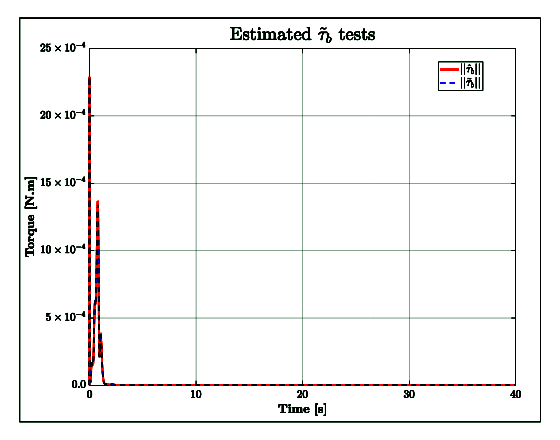
\includegraphics[width=\textwidth]{graphs/tau-body-2}
%\caption{Initial torque response spike}
%\label{fig:tau-body-2}
%\end{subfigure}
%\begin{subfigure}{0.49\textwidth}
%\centering
%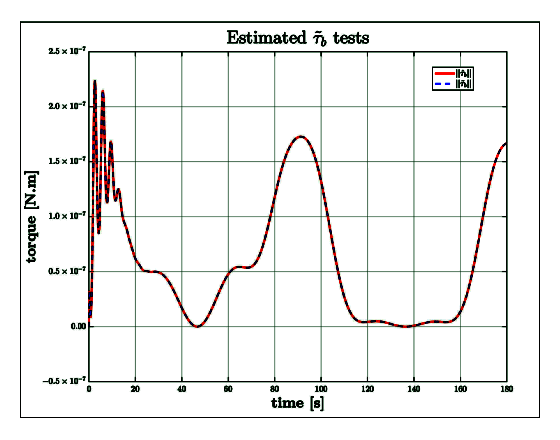
\includegraphics[width=\textwidth]{graphs/tau-body}
%\caption{Steady state torque response}
%\label{fig:tau-body-1}
%\end{subfigure}
%\vspace{-6pt}
%\caption{Approximated and true body torque responses}
%\label{fig:tau-body}
%\vspace{-16pt}
%\end{figure}
%\par
%Sample rates of $100~\text{Hz}$ were used to calculate the instantaneous inertia values throughout the trajectory. Initial torques spike from time $t_0\rightarrow 2~\text{s}$ occurs as the vehicle first steps to the attitude setpoint from rest, with an attitude at the origin, shown in Fig:\ref{fig:tau-body-2}. Once the vehicle reaches steady state trajectory tracking the induced torque reduces dramatically, plotted for a longer time Fig:\ref{fig:tau-body-1}. The plot for $\color{blue}\norm{\tilde{\tau}_b(u)}$ uses discrete time derivatives as per Eq:\ref{eq:discrete-inertia-approximation}.
%\par
%Fig:\ref{fig:tau-body-r} shows the error between $\color{red}\norm{\vec{\tau}_b(u)}$ and approximated $\color{blue}\norm{\tilde{\tau}_b(u)}$, again the initial spike is from starting configuration changes; thereafter the error reduces dramatically. On average the approximation asserted in Eq:\ref{eq:discrete-inertia-approximation} is a reasonable one with an error typically three orders of magnitude smaller than the signal it represents, or $\times 10^{-3}~\text{Nm}$, less than the torque $\vec{\tau}_b(u)$. The transfer block for the dynamics in simulation still make use of a continuous time derivative model whilst plant dependent controller compensation uses a reduced complexity approximation\ldots
%\begin{figure}[hbtp]
%\centering
%\begin{subfigure}{0.49\textwidth}
%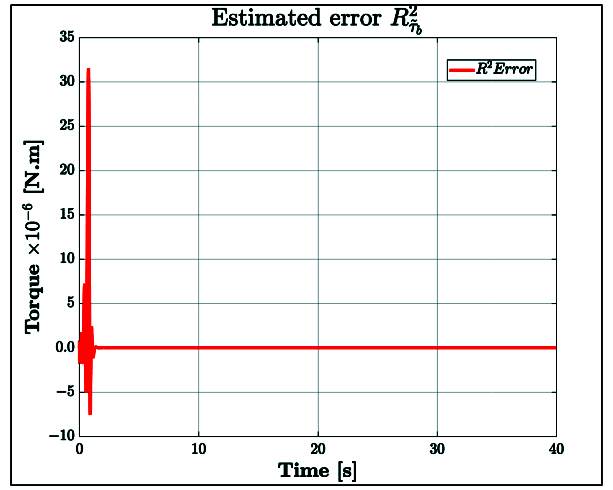
\includegraphics[width=\textwidth]{graphs/tau-body-r-2}
%\caption{Initial step torque error}
%\label{fig:tau-body-r-2}
%\end{subfigure}
%\begin{subfigure}{0.49\textwidth}
%\centering
%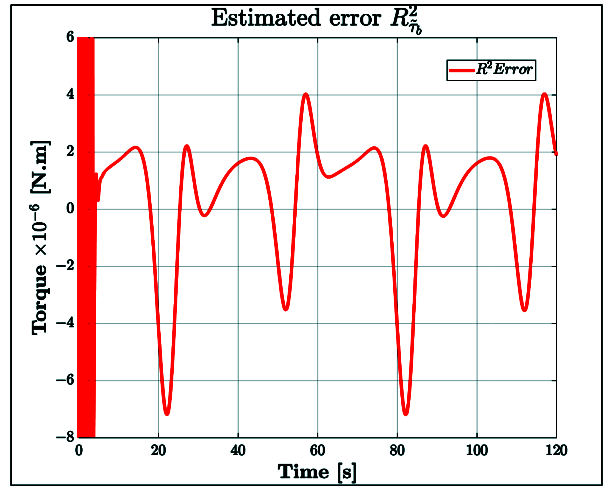
\includegraphics[width=\textwidth]{graphs/tau-body-r}
%\caption{Steady state torque error}
%\label{fig:tau-body-r-1}
%\end{subfigure}
%\caption{Approximated and true body torque responses}
%\label{fig:tau-body-r}
%\vspace{-14pt}
%\end{figure}
%\par
%Any measurement or modelling errors associated with the above inertial response models and their explicit values presented in Sec:\ref{sec:proto.inertia} can easily be compensated for as plant disturbances. More specifically errors in the above system are modelled as plant dependent state uncertainties; and could be adaptively compensated for accordingly.
%====================================================
\subsection{Verification and simulation of induced model}
\label{subsec:dynamics.nonlinearities.torque-tests}
%====================================================
%\subsubsection{Linearization simulation and comparison}
%Previously in Sec:\ref{subsec:dynamics.nonlinearities.gyrotorques} the proposed Lagrangian energy functions for both $\Delta\lambda_i$ and $\Delta\alpha_i$ servo rotations and their response to body angular velocities $\vec{\omega}_b$ were derived. Recalling those equations; the inner ring net (kinetic) energy Lagrangian from Eq:\ref{eq:lagrange-inner} is:
%\begin{subequations}
%\begin{equation}\label{eq:sim-lagrange-inner}
%\mathcal{L}_{n/m}=\frac{1}{2}\vec{\omega}_{r/m}\text{}^T\big(J_{r}'\big)\vec{\omega}_{r/m}+\frac{1}{2}\vec{\omega}_{n/m}\text{}^T\big(J_{ir}'\big)\vec{\omega}_{n/m}
%\end{equation}
%\vspace{-16pt}
%\begin{equation}\label{eq:sim-lagrange-inner-expand}
%=\frac{1}{2}\Big(R_x(\lambda)\vec{\Omega}_i+\dot{\vec{\lambda}}_i\Big)^{T}\Big(R_x(\lambda)\big(J_r\big)R_x^{-1}(\lambda)\Big)\Big(R_x(\lambda)\vec{\Omega}_i+\dot{\vec{\lambda}}_i\Big)+\frac{1}{2}\big(\dot{\vec{\lambda}}_i\big)^T\Big(R_x(\lambda)\big(J_{ir}\big)R_x^{-1}(\lambda)\Big)\big(\dot{\vec{\lambda}}_i\big)
%\end{equation}
%And similarly for the middle ring's net (kinetic) energy from Eq:\ref{eq:alpha-lagrange}:
%\begin{equation}\label{eq:sim-lagrange-middle}
%\mathcal{L}_{m/p}=\frac{1}{2}\vec{\omega}_{r/p}^{\hspace{2pt}T}\big(J_{r}''\big)\vec{\omega}_{r/p}+\frac{1}{2}\vec{\omega}_{n/p}^{\hspace{2pt}T}\big(J_{ir}''\big)\vec{\omega}_{n/p}+\frac{1}{2}\vec{\omega}_{m/p}^{\hspace{2pt}T}\big(J_{m}'\big)\vec{\omega}_{m/p}
%\end{equation}
%\vspace{-14pt}
%\begin{multline}\label{eq:sim-lagrange-middle-expand}
%=\frac{1}{2}\Big(R_y(\alpha)R_x(\lambda)\vec{\Omega}_i+R_y(\alpha)\dot{\vec{\lambda}}_i+\dot{\vec{\lambda}}_i\Big)^T\Big(R_y(\alpha)\big(J_r'\big)R_y^{-1}(\alpha)\Big)\Big(R_y(\alpha)R_x(\lambda)\vec{\Omega}_i+R_y(\alpha)\dot{\vec{\lambda}}_i+\dot{\vec{\alpha}}_i\Big)
%\\
%\frac{1}{2}\Big(R_y(\alpha)\dot{\vec{\lambda}}_i+\dot{\vec{\alpha}}_i\Big)^T\Big(R_y(\alpha)\big(J_{ir}'\big)R_y^{-1}(\alpha)\Big)\Big(R_y(\alpha)\dot{\vec{\lambda}}_i+\dot{\vec{\alpha}}_i\Big)
%\\
%+\frac{1}{2}\Big(\dot{\vec{\alpha}}_i\Big)^T\Big(R_y(\alpha)\big(J_m\big)R_y^{-1}(\alpha)\Big)\Big(\dot{\vec{\alpha}}_i\Big)
%\end{multline}
%\end{subequations}
%Solving for the generalized forces acting on each system requires application of Euler-Lagrange formulation, using partial derivatives relative to generalized path coordinates. Both the inner and middle ring systems were defined with relative coordinate paths for the angular servo position $\vec{\mathbf{u}}=\begin{bmatrix}\lambda_i&0&0\end{bmatrix}^T$ and $\vec{\mathbf{v}}=\begin{bmatrix}0&\alpha_i&0\end{bmatrix}^T$ respectively. The generalized forces for both systems are then, using the Euler-Lagrange formulation:
%\begin{equation}\label{eq:sim-lagranges}
%\underbrace{\frac{d}{dt}\bigg(\frac{\partial\mathcal{L}_{n/m}}{\partial\dot{\vec{\mathbf{u}}}}\bigg)-\frac{\partial\mathcal{L}_{n/m}}{\partial\vec{\mathbf{u}}}=\vec{\mathbf{U}}(\lambda_i)}_{\text{Inner ring}}~~\text{and}~~\underbrace{\frac{d}{dt}\bigg(\frac{\partial\mathcal{L}_{m/p}}{\partial\dot{\vec{\mathbf{v}}}}\bigg)-\frac{\partial\mathcal{L}_{m/p}}{\partial\vec{\mathbf{v}}}=\vec{\mathbf{V}}(\lambda_i,\alpha_i)}_{\text{Middle ring}}
%\end{equation}
%The assumption proposed in Eq:\ref{eq:rotation-linear}, presented in \cite{rotationlinearize}, is used to linearize and reduce partial derivatives of the respective inner and middle ring Lagrangians in Eq:\ref{eq:sim-lagranges}. Those simplifications are such that both terms in Eq:\ref{eq:sim-lagranges} respectively simplify to:
%\begin{equation}\label{eq:sim-lagranges-linear}
%\frac{d}{dt}\bigg(\frac{\partial\mathcal{L}_{n/m}}{\partial\dot{\vec{\mathbf{u}}}}\bigg)=\vec{\mathbf{U}}(\lambda_i)~\Big|_{\big(\partial\mathcal{L}_{n/m}/\partial\vec{\mathbf{u}}\big)\approx 0}~~\text{and}~~\frac{d}{dt}\bigg(\frac{\partial\mathcal{L}_{m/p}}{\partial\dot{\vec{\mathbf{v}}}}\bigg)=\vec{\mathbf{V}}(\alpha_i,\lambda_i)\Big|_{\big(\partial\mathcal{L}_{m/p}/\partial\vec{\mathbf{v}}\big)\approx 0}
%\end{equation}
%Considering first the case of the inner ring Lagrangian $\mathcal{L}_{n/m}$ from Eq:\ref{eq:sim-lagrange-inner-expand} relative to the middle ring frame $\mathcal{F}^{M_i'}$; the partial derivative taken with respect to path variable $\vec{\mathbf{u}}=\vec{\lambda}_i$ was simplified:
%\begin{equation}\label{eq:sim-lagrange-inner-simple}
%\frac{\partial\mathcal{L}_{n/m}}{\partial\vec{\mathbf{u}}}=\frac{\partial}{\partial\vec{\lambda}_i}\big(\mathcal{L}_{n/m}\big)\approx 0
%\end{equation}
%Expanding Eq:\ref{eq:sim-lagrange-inner-simple} and finding the partial derivative of that Lagrangian, $\mathcal{L}_{n/m}$ in Eq:\ref{eq:sim-lagrange-inner-expand}, with respect to $\vec{\mathbf{u}}=\vec{\lambda}_i$ yields:
%\begin{multline}\label{eq:3.118}
%\frac{\partial\mathcal{L}_{n/m}}{\partial\vec{\mathbf{u}}}=\frac{\partial\mathcal{L}_{n/m}}{\partial\vec{\lambda}_i}=\frac{1}{2}\bigg(\frac{\partial}{\partial\vec{\lambda}_i}\Big(R_x(\lambda)\vec{\Omega}_i\Big)\bigg)^T\Big(R_x(\lambda)\big(J_r\big)R_x^{-1}(\lambda)\Big)\Big(R_x(\lambda)\vec{\Omega}_i+\dot{\vec{\lambda}}_i\Big)
%\\
%+\frac{1}{2}\Big(R_x(\lambda)\vec{\Omega}_i+\dot{\vec{\lambda}}_i\Big)^T\bigg(\frac{\partial}{\partial\vec{\lambda}_i}\Big(R_x(\lambda)\big(J_r\big)R_x^{-1}(\lambda)\Big)\bigg(R_x(\lambda)\vec{\Omega}_i+\dot{\vec{\lambda}}_i\Big)
%\\
%+\frac{1}{2}\Big(R_x(\lambda)\vec{\Omega}_i+\dot{\vec{\lambda}}_i\Big)^T\Big(R_x(\lambda)\big(J_r\big)R_x^{-1}(\lambda)\Big)\bigg(\frac{\partial}{\partial\vec{\lambda}_i}\Big(R_x(\lambda)\vec{\Omega}_i\Big)\bigg)
%\\
%+\frac{1}{2}\Big(\dot{\vec{\lambda}}_i\Big)^T\bigg(\frac{\partial}{\partial\vec{\lambda}_i}\Big(R_x(\lambda)\big(J_{ir}\big)R_x^{-1}(\lambda)\Big)\bigg)\Big(\dot{\vec{\lambda}}_i\Big)
%\end{multline}
%Testing that assumption, presented in Eq:\ref{eq:rotation-linear}; the partial derivative components of Eq:\ref{eq:3.118} are explicitly calculated. First, considering the rotor's transformed inertia $J_r'=R_x(\lambda)\big(J_r\big)R_x^{-1}(\lambda)$ with a partial derivative as per the differential product rule:
%\begin{subequations}
%\begin{equation}
%\frac{\partial}{\partial\vec{\mathbf{u}}}\big(J_r'\big)= \frac{\partial}{\partial\vec{\lambda}_i}\bigg(R_x(\lambda)\big(J_r\big)R_x^{-1}(\lambda)\bigg)
%\end{equation}
%\vspace{-4pt}
%\begin{equation}\label{eq:sim-inner-partial-rotor}
%=\frac{\partial}{\partial\vec{\lambda}_i}\Big(R_x(\lambda)\Big)\big(J_r\big)R_x^{-1}(\lambda)+R_x(\lambda)\big(J_r\big)\frac{\partial}{\partial\vec{\lambda}_i}\Big(R_x^{-1}(\lambda)\Big)
%\end{equation}
%Similarly for the inner ring transformed inertia's contribution, $J_{ir}'=R_x(\lambda)\big(J_{ir}\big)R_x^{-1}(\lambda)$ from Eq:\ref{eq:sim-lagrange-inner-expand}, however, \emph{without} including the rotor body's inertia:
%\begin{equation}\label{eq:sim-inner-partial-inner}
%\frac{\partial}{\partial\vec{\mathbf{u}}}\big(J_{ir}'\big)=\frac{\partial}{\partial\vec{\lambda}_i}\Big(R_x(\lambda)\Big)\big(J_{ir}\big)R_x^{-1}(\lambda)+R_x(\lambda)\big(J_{ir}\big)\frac{\partial}{\partial\vec{\lambda}_i}\Big(R_x^{-1}(\lambda)\Big)
%\end{equation}
%The final partial derivative to take note of is that for the rotor's angular velocity $\vec{\Omega}_i$, in $\text{rad.s}^{-1}$, but transformed to the inner ring frame $\mathcal{F}^{M_i'}$ which the Lagrangian in Eq:\ref{eq:sim-lagrange-inner} is taken with respect to:
%\begin{equation}\label{eq:sim-inner-partial-angular}
%\frac{\partial}{\partial\vec{\lambda}_i}\Big(R_x(\lambda)\vec{\Omega}_i\Big)
%\end{equation}
%\end{subequations}
%The application of the rotation matrix linearization, from Eq:\ref{eq:rotation-linear}, to the partial derivative rotations in Eq:\ref{eq:sim-inner-partial-rotor}-\ref{eq:sim-inner-partial-angular} is:
%\begin{subequations}
%\begin{equation}\label{eq:sim-rot-linear}
%R_x(\bar{\lambda}_i+\partial\lambda_i)\approx\Big(1-[\Phi_x(\bar{\lambda}_i)\partial\lambda_i]_\times\Big)R_x(\bar{\lambda}_i)
%\end{equation}
%Where $\Phi_x(\bar{\lambda}_i)$ is simply the partial derivative of the Euler matrix, $\Phi(\eta)$ from Eq:\ref{eq:angular-rates.f}, with respect to an $\hat{X}$ axis rotation. That being:
%\begin{equation}
%\Phi_x(\bar{\lambda}_i)=\begin{bmatrix}
%0 & 0 & 0\\
%0 & \sin{\bar{\lambda}}_i & \cos{\bar{\lambda}}_i\\
%0 & -\cos{\bar{\lambda}}_i & \sin{\bar{\lambda}}_i
%\end{bmatrix}
%\end{equation}
%So then, for some nominal angle $\bar{\lambda}_i$ perturbed by some small deviation $\partial\lambda_i$, Eq:\ref{eq:sim-rot-linear} expands to:
%\begin{equation}
%\therefore R_x(\bar{\lambda}_i+\partial\lambda_i)\approx R_x(\bar{\lambda}_i)-\begin{bmatrix}
%0 & 0 & 0\\
%0 & \big(c^2\bar{\lambda}_i-s^2\bar{\lambda}_i\big) & \big(-c\bar{\lambda}_is\bar{\lambda}_i-s\bar{\lambda}_ic\bar{\lambda}_i\big)\\
%0 & \big(s\bar{\lambda}_ic\bar{\lambda}_i+c\bar{\lambda}_is\bar{\lambda}_i\big) & \big(c^2\bar{\lambda}_i-s^2\bar{\lambda}_i\big)
%\end{bmatrix}\partial\lambda_i
%\end{equation}
%Which, obviously, when the perturbation $\partial\lambda_i$ away from the nominal $\bar{\lambda}_i$ is small, it follows that:
%\begin{equation}
%\rightarrow R_x(\bar{\lambda}_i+\partial\lambda_i)\approx R_x(\bar{\lambda}_i)\Big|_{\partial\lambda_i<<1}
%\end{equation}
%\end{subequations}
%That simplification then applies to Eq:\ref{eq:sim-inner-partial-rotor},\ref{eq:sim-inner-partial-inner} and \ref{eq:sim-inner-partial-angular}, for a small $\partial\lambda_i$:
%\begin{subequations}\label{eq:inner-ring-linearizations}
%\begin{equation}
%\frac{\partial}{\partial\vec{\lambda}_i}J_r'\approx 0
%\end{equation}
%\vspace{-8pt}
%\begin{equation}
%\frac{\partial}{\partial\vec{\lambda}_i}J_{ir}'\approx 0
%\end{equation}
%\vspace{-6pt}
%\begin{equation}
%\frac{\partial}{\partial\vec{\lambda}_i}R_x(\lambda)\vec{\Omega}_i\approx 0
%\end{equation}
%\end{subequations}
%It can therefore be said that the assumption in Eq:\ref{eq:sim-lagrange-inner-simple} is not without merit, or that:
%\begin{equation}
%\frac{\partial\mathcal{L}_{n/m}}{\partial\vec{\mathbf{u}}}\approx 0\rightarrow\frac{d}{dt}\bigg(\frac{\partial\mathcal{L}_{n/m}}{\partial\dot{\vec{\mathbf{u}}}}\bigg)-\frac{\partial\mathcal{L}_{n/m}}{\partial\vec{\mathbf{u}}}\approx\frac{d}{dt}\Big(\frac{\partial\mathcal{L}_{n/m}}{\partial\dot{\vec{\lambda}}_i}\Big)=\vec{\mathbf{U}}(\lambda_i)=\vec{\tau}_\lambda(\lambda_i)~~~~\in\mathcal{F}^{M_i'}
%\end{equation}
%\par
%A final verification of the proposed rotation matrix approximation is done with a \textbf{Simulink} model whose structure is shown in Fig:\ref{fig:linear-block}. The model applies a direct comparison of $\vec{\tau}_\lambda(\lambda_i)$, originally from Eq:\ref{eq:torque-induced-inner}, both \emph{with} and \emph{without} the rotation matrix linearizations in Eq:\ref{eq:inner-ring-linearizations}. Convention has it that estimated or approximated values are denoted with a hat accent. Therefore a calculated inner ring torque response, \emph{with linearized} partial derivatives as per Eq:\ref{eq:inner-ring-linearizations}, is termed as $\hat{\tau}_\lambda(\lambda_i)$. The simulated representation of the induced torque response \emph{without} applied linearizations, $\vec{\tau}_\lambda$, is calculated from the block model detailed in Fig:\ref{fig:linear-block}. The complete inner ring Euler-Lagrange formulation is calculated from Eq:\ref{eq:sim-lagranges}.
%\par
%\begin{figure}[htbp]
%\vspace{-4pt}
%\centering
%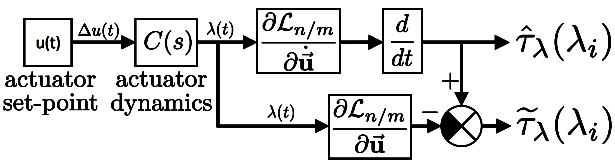
\includegraphics[width=0.75\textwidth]{figs/linear-block}
%\caption{Simulink Lagrangian block}
%\label{fig:linear-block}
%\vspace{-6pt}
%\end{figure}
%\par
%The block $u(t)$ in Fig:\ref{fig:linear-block} represents some commanded change in actuator position, within the actuator space $u\in\mathbb{U}$. That space consists of propeller speeds $\Omega_i$ and servo positions $\lambda_i$ and $\alpha_i$ for $i\in[1:4]$; as detailed in Eq:\ref{eq:actuator-space}. Each actuator has its own transfer function, driven by the collective dynamic block $C(s)$, with transfer characteristics determined in Sec:\ref{subsec:proto.design.transfer}. That actuator argument $u(t)$ then leads to some time varying inner ring servo position $\lambda_i(t)$, with a rate $\dot{\lambda}_i(t)$. Both of which are used to calculate the complete Euler-Lagrangian equation:
%\begin{equation}\label{eq:sim-lagrange-torque-inner}
%\frac{d}{dt}\bigg(\frac{\partial\mathcal{L}_{n/m}}{\partial\dot{\vec{\mathbf{u}}}}\bigg)-\frac{\partial\mathcal{L}_{n/m}}{\partial\vec{\mathbf{u}}}=\vec{\tau}_\lambda(\lambda_i)
%\end{equation}
%Seeing that Eq:\ref{eq:sim-lagrange-torque-inner} produces a 3-D vector result and not a scalar; vector magnitudes $\norm{\vec{\tau}_\lambda(\lambda_i)}$ and $\norm{\hat{\tau}_\lambda(\lambda_i)}$ are considered. The objective here is to quantify the effect a rotation matrix linearization has on the estimated generalized torque calculations detailed above.
%\par
%\begin{figure}[hbtp]
%\centering
%\begin{subfigure}{0.49\textwidth}
%\centering
%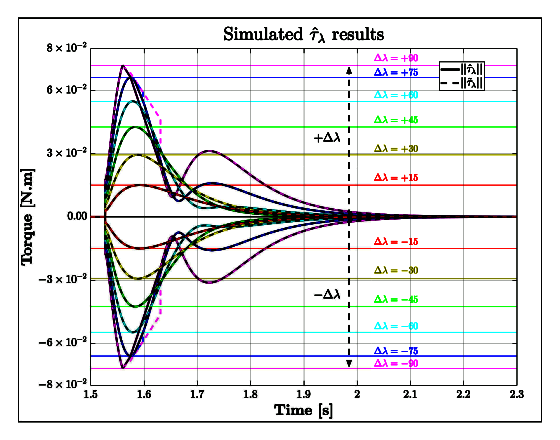
\includegraphics[width=\textwidth]{graphs/tau-lambda-hat}
%\caption{$\norm{\vec{\tau}_\lambda(\lambda_i)}$ and linearized $\norm{\hat{\tau}_\lambda(\lambda_i)}$ step responses}
%\label{fig:tau-lambda-hat}
%\end{subfigure}
%\begin{subfigure}{0.49\textwidth}
%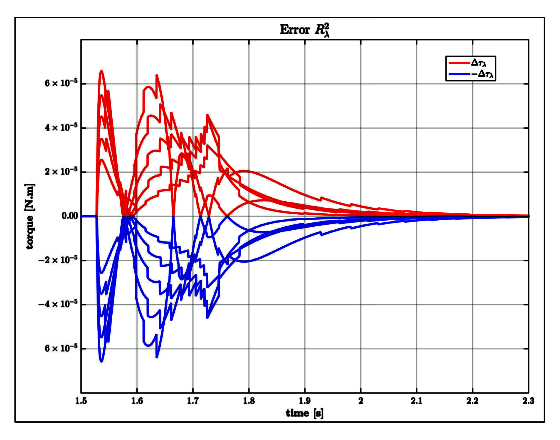
\includegraphics[width=\textwidth]{graphs/tau-lambda-hat-r}
%\caption{$R^2_\lambda$ error for linearized response}
%\label{fig:tau-lambda-hat-r}
%\end{subfigure}
%\caption{Inner ring induced torque responses for $\Delta\lambda_i$}
%\vspace{-10pt}
%\label{fig:tau-lambda-sim}
%\vspace{-6pt}
%\end{figure}
%\par
%Plotted in Fig:\ref{fig:tau-lambda-hat} are both estimated $\norm{\hat{\tau}_\lambda(\lambda_i)}$ and simulated $\norm{\vec{\tau}_\lambda(\lambda_i)}$ torques, calculated with a nominal constant angular propeller speed $\Omega_i=6000~\text{RPM}$. Increasing positive and negative step sizes for changes in $\Delta\lambda_i$ are shown, resulting in greater torque responses.  The $R^{2}_\lambda$ error between $\norm{\vec{\tau}_\lambda(\lambda_i)}$ and $\norm{\hat{\tau}_\lambda(\lambda_i)}$ is plotted in Fig:\ref{fig:tau-lambda-hat-r}. That difference between $\norm{\vec{\tau}_\lambda(\lambda_i)}$ and $\norm{\hat{\tau}_\lambda(\lambda_i)}$ is precisely the partial derivative contribution $\partial\mathcal{L}_{n/m}/\partial\vec{\mathbf{u}}$. Or rather mathematically:
%\begin{subequations}\label{eq:error-tau-r}
%\begin{equation}
%R^2_\lambda\triangleq\norm{\vec{\tau}_\lambda(\lambda_i)}-\norm{\hat{\tau}_\lambda(\lambda_i)}
%\end{equation}
%\vspace{-14pt}
%\begin{equation}
%=\norm{\Bigg(\frac{d}{dt}\bigg(\frac{\partial\mathcal{L}_{n/m}}{\partial\dot{\vec{\mathbf{u}}}}\bigg)\Bigg)}-\norm{\Bigg(\frac{d}{dt}\bigg(\frac{\partial\mathcal{L}_{n/m}}{\partial\dot{\vec{\mathbf{u}}}}\bigg)-\frac{\partial\mathcal{L}_{n/m}}{\partial\vec{\mathbf{u}}}\Bigg)}
%\end{equation}
%\begin{equation}
%\therefore R^2_\lambda=\norm{\frac{\partial\mathcal{L}_{n/m}}{\partial\vec{\mathbf{u}}}}
%\end{equation}
%\end{subequations}
%\par
%The simulation for $R^2_\lambda$ suffered from tolerance errors within the MatLab integral approximator, this was as a result of the small deviations which were being calculated. Despite that; the differences, using the inertial matrices and dimensions defined for the prototype in Sec:\ref{sec:proto.inertia}, were typically in the order of $\times 10^{-5}~~\text{Nm}$ for steps in $\Delta\lambda_i$. 
%\par
%Only for large angular changes in $\Delta\lambda_i$ does the approximation begin to deteriorate. Mostly both $\hat{\tau}_\lambda(\lambda_i)$ and $\tilde{\tau}_\lambda(\lambda_i)$ were three orders of magnitude greater than their errors; torques were in the range of $\times 10^{-2}~~\text{Nm}$. The error for when $\lambda_i=\pi/2$ was not included in Fig:\ref{fig:tau-alpha-hat-r} because it was the only error which did not fit on the $\times 10^{-5}~\text{Nm}$ scale, being an order of magnitude greater.
%\par
%The same process was then applied to the middle ring Lagrangian $\mathcal{L}_{m/p}$ relative to the intermediate frame $\mathcal{F}^{M_i''}$, from Eq:\ref{eq:sim-lagrange-middle-expand} to evaluate $\vec{\tau}_\alpha(\lambda_i,\alpha_i)$. Those results are plotted collectively in Fig:\ref{fig:tau-alpha-sim}. Note that both $\norm{\vec{\tau}_\alpha(\lambda_i,\alpha_i)}$ and $\norm{\hat{\tau}_\alpha(\lambda_i,\alpha_i)}$ are plotted, \underline{not the generalized torques} $\vec{\mathbf{V}}(\lambda_i,\alpha_i)$ acting on the system. The generalized torque response $\vec{\mathbf{V}}(\lambda_i,\alpha_i)$ from Eq:\ref{eq:sim-lagranges} and expanded in Eq:\ref{eq:3.86g} \underline{includes the inner ring's energy contribution} $\vec{\mathbf{U}}(\lambda_i)$ or $\vec{\tau}_\lambda(\lambda_i)$; whilst $\vec{\tau}_\alpha(\lambda_i,\alpha_i)$ and $\hat{\tau}_\alpha(\lambda_i,\alpha_i)$ do not. From Eq:\ref{eq:torque-induced-middle}, $\vec{\tau}_\alpha(\lambda_i,\alpha_i)$ is defined as a function of $\vec{\mathbf{V}}(\lambda_i,\alpha_i)$ and $\vec{\mathbf{U}}(\lambda_i)$:
%\begin{equation}
%\vec{\tau}_\alpha(\lambda_i)\triangleq \vec{\mathbf{V}}(\lambda_i,\alpha_i)-R_y(\lambda)\vec{\mathbf{U}}(\lambda_i)
%\end{equation}
%Plots for the net generalized torque response $\vec{\mathbf{V}}(\lambda_i,\alpha_i)$ acting on the system with combined changes for $\Delta\alpha_i$ and $\Delta\lambda_i$ are included in App:\ref{app:tau-comb}. Moreover only a constant value for the $\lambda_i$ servo position was used for the tests in Fig:\ref{fig:tau-alpha-sim}. The same constant propeller speed $\Omega_i=6000~\text{RPM}$ was used together with a constant $\lambda_i=0~\text{rad}$ for the inner ring's servo, maintaining a constant inner ring inertia contribution.
%\par
%\begin{figure}[htbp]
%\centering
%\begin{subfigure}{0.49\textwidth}
%\centering
%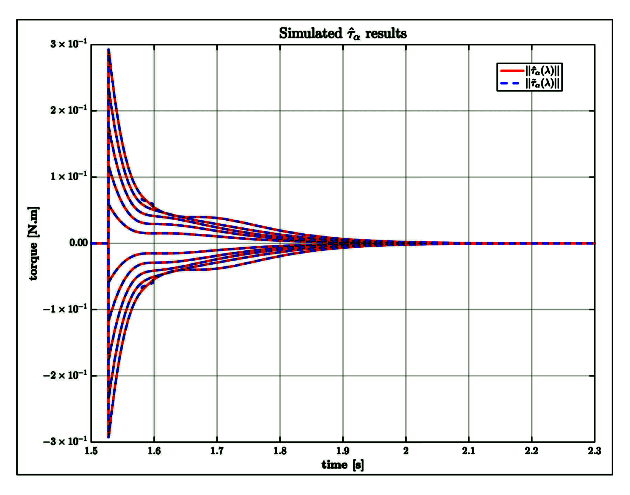
\includegraphics[width=0.95\textwidth]{graphs/tau-alpha-hat}
%\caption{$\norm{\vec{\tau}_\alpha(\lambda_i,\alpha_i)}$ and linearized $\norm{\hat{\tau}_\alpha(\lambda_i,\alpha_i)}$}
%\label{fig:tau-alpha-hat}
%\end{subfigure}
%\begin{subfigure}{0.49\textwidth}
%\centering
%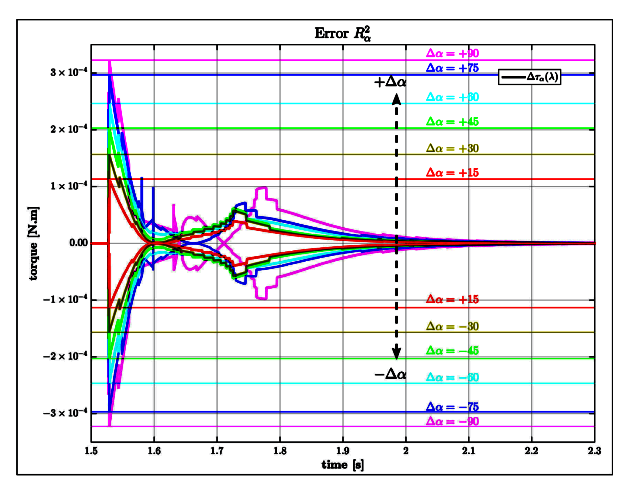
\includegraphics[width=0.95\textwidth]{graphs/tau-alpha-hat-r}
%\caption{$R^2_\alpha$ error for linearized responses}
%\label{fig:tau-alpha-hat-r}
%\end{subfigure}
%\vspace{-4pt}
%\caption{Middle ring induced torque responses for $\Delta\alpha_i$}
%\label{fig:tau-alpha-sim}
%\vspace{-16pt}
%\end{figure}
%\par
%The initial torque spike in $\vec{\tau}_\alpha(\lambda_i,\alpha_i)$ shown in Fig:\ref{fig:tau-alpha-hat} is as a result of the significantly larger rotational inertia, $J_{p}(\lambda_i)$ for the entire motor module in Eq:\ref{eq:inertia.middle.b}, encountered by a second order angular acceleration $\ddot{\alpha}_i$. That response is depreciated in the case of the inner ring for $\vec{\tau}_\lambda(\lambda_i)$ because of how much smaller that rotational inertia, $J_n$ for the inner ring only in Eq:\ref{eq:inertia.inner}, physically is. As per power calculations for the servo using parameters from Sec:\ref{subsec:proto.design.transfer}; the servo's angular acceleration is rate limited to $472~\text{rad.s}^{-2}$, but neither tests come close to reaching saturation.
%\par
%The second torque peak which begins to manifest in the inner ring response for $\vec{\tau}_\lambda(\lambda_i)$ shown in Fig:\ref{fig:tau-lambda-hat} is as a result of the angular velocity rate limit $\dot{\lambda}_{max}=7.4799~\text{rad.s}^{-1}$ being encountered. The same limit is encountered for the middle ring response $\vec{\tau}_\alpha(\lambda_i,\alpha_i)$ in Fig:\ref{fig:tau-alpha-hat} but is far less significant in relation to the initial second order acceleration torque peak. The deviation between $\norm{\vec{\tau}_\alpha(\lambda_i,\alpha_i)}$ and $\norm{\hat{\tau}_\alpha(\lambda_i,\alpha_i)}$ is only of the order of $10^{-4}~\text{Nm}$ whilst typical induced torque values are again three orders of magnitude greater, or of the order $10^{-1}~\text{Nm}$. Only at large angular changes for either $\Delta\lambda_i$ or $\Delta\alpha_i$ do the simplifications proposed begin to deteriorate.
%\par
%Note that gravitational torque contributions are not included in either of the above tests for $\vec{\tau}_\lambda(\lambda_i)$ in Eq:\ref{eq:torque-induced-inner} or $\vec{\tau}_\alpha(\lambda_i,\alpha_i)$ in Eq:\ref{eq:torque-induced-middle}. Plots in both Fig:\ref{fig:tau-lambda-hat} and Fig:\ref{fig:tau-alpha-hat} show the linearizations applied in Eq:\ref{eq:sim-lagranges-linear} hold true for most $\Delta\lambda_i$ or $\Delta\alpha_i$ steps; typically having an error three orders of magnitude smaller than the induced response considered. The control loop will only ever be dealing with minor step size changes for servo positions and so, the linearization is an appropriate one that will reduce interval computational complexity.
\subsubsection{Dynamic model verification}
\label{subsubsec:dynamicmodel}
In spite of the rigorous mathematical approached applied to the multibody system above, physical corroboration of the proposed model(s) is still required. The systems described in Eq:\ref{eq:torque-induced-inner} for $\vec{\tau}_\lambda(\lambda_i)$, Eq:\ref{eq:torque-induced-middle} for $\vec{\tau}_\alpha(\lambda_i,\alpha_i)$ and Eq:\ref{eq:net-body-response} for $\vec{\tau}_b(u)$ require further verification before an accurate and reliable simulation can be constructed based upon them. Two test rigs were designed and constructed (Fig:\ref{fig:torque-inner} and Fig\ref{fig:torque-middle}) to physically measure the induced torques in question. The first test rig recreates the relative motion of the inner ring actuated by the $\lambda_i$ servo. Similarly the second test platform mimics the middle ring's response when driven by the outer $\alpha_i$ servo. 
\par
The net body response, $\vec{\tau}_b(u)$ relating to net angular body velocity $\vec{\omega}_b$ in Eq:\ref{eq:net-body-response}, is harder to recreate on an isolated test rig. Such results are only discussed in the context of simulation. Considering first the inner most ring assembly; Fig:\ref{fig:torque-inner} shows the test rig used to isolate and measure $\vec{\tau}_\lambda(\lambda_i)$ responses to $\Delta\lambda_i$ rotations. The inner ring is supported by two bearing assemblies; an extended shaft in the $-\hat{X}_{M_i}$ direction connects the inner ring to the driving servo block.
\par
\begin{figure}[htpb]
\centering
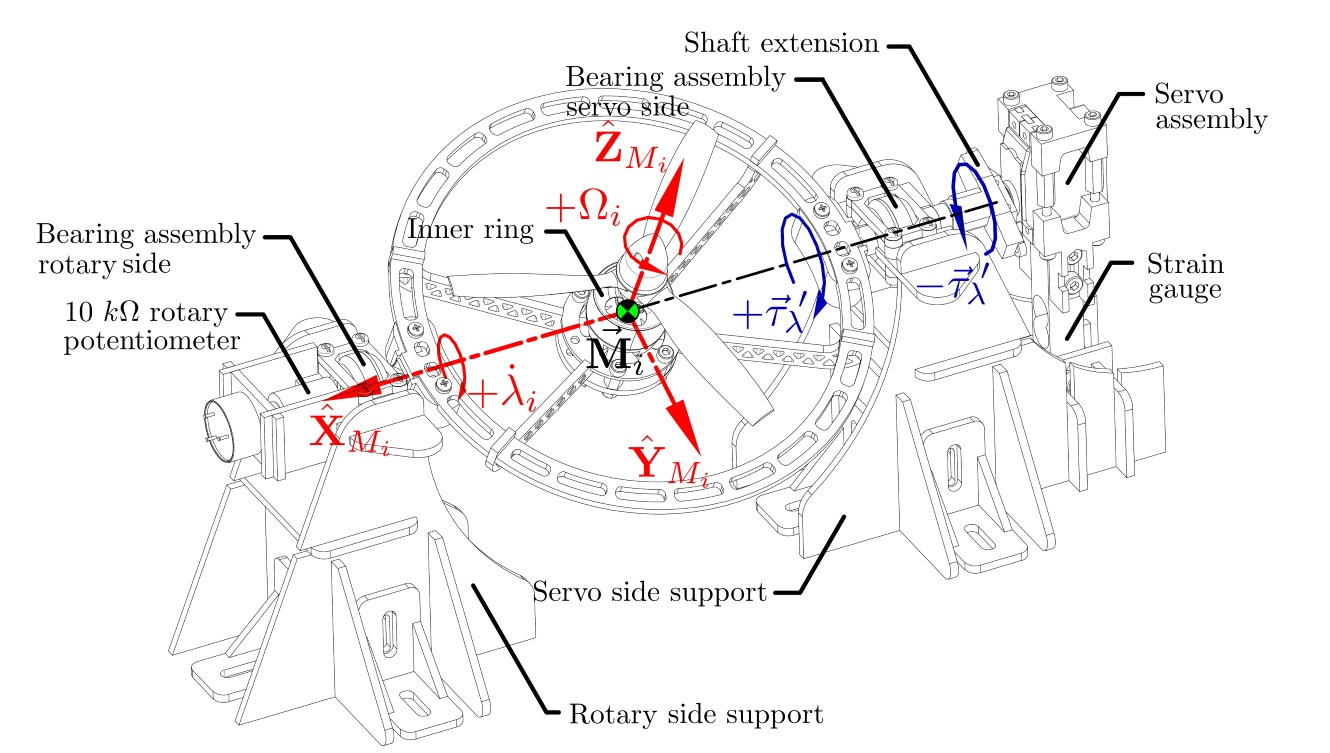
\includegraphics[width=\textwidth]{figs/torque-inner}
\caption{Inner ring torque test rig}
\label{fig:torque-inner}
\vspace{-12pt}
\end{figure}
\par
Physical rotational torque $\vec{\tau}_\lambda(\lambda_i)$ is transferred through the shaft extension from the servo to the inner ring. The servo block is secured only by a vertically aligned and calibrated strain gauge (App:\ref{app:strain}). Deflection of the strain gauge is then proportional to the torque applied by the servo to rotate the inner ring structure. It is important to mention that, whilst the bearing assembly facilitates the transfer of the servo's rotational torque, the assembly isolates only the $\hat{X}_{M_i'}$ component of the induced torque. If $\vec{\tau}_{\lambda}\text{}\hspace{-2pt}'$ is the deflection torque physically measured; its relationship with the induced torque vector $\vec{\tau}_{\lambda}(\lambda_i)$ is given by:
\begin{equation}\label{eq:tau-lambda-prime}
\vec{\tau}_{\lambda}\text{}\hspace{-2pt}'=\vec{\tau}_{\lambda}(\lambda_i)\cdot\hat{X}_{M_i'}~~~~\in\mathcal{F}^{M_i'}
\end{equation}
One final thing to consider is that the modelled equation for $\vec{\tau}_\lambda(\lambda_i)$, previously in Eq:\ref{eq:torque-induced-inner}, \emph{does not} account for the gravitational torque from an eccentric center of gravity (Fig:\ref{fig:inertia-inner}) or induced aerodynamic torque about the propellers hub (Fig:\ref{fig:torques} and Eq:\ref{eq:bem-power}). The derivations earlier in Sec:\ref{subsec:dynamics.nonlinearities.gyrotorques} introduce net gravitational torque for an effective center of gravity $\vec{\tau}_g$ into Eq:\ref{eq:3.110a}. Moreover aerodynamic drag $\vec{H}(\Omega_i)$ about the propeller's rotational axis is to be included as an additive term. 
\par
The torque response $\vec{\tau}_\lambda(\lambda_i)$ opposed to changes of $\Delta\lambda_i$, and hence the servo's acceleration $\ddot{\lambda}_i$ is then, from Eq:\ref{eq:torque-induced-inner} with introduced gravitational and aerodynamic drag torque components relative to the middle ring frame $\mathcal{F}^{M_i'}$:
\begin{multline}\label{eq:model-inner}
\vec{\tau}_\lambda(\lambda_i)=\big(\dot{J}_{r}'\big)\vec{\Omega}_i\text{}\hspace{-2pt}'+\big(\dot{J}_{n}'\big)\dot{\vec{\lambda}}_i+\big(J_r'\big)\dot{\vec{\Omega}}_i\text{}\hspace{-2pt}'+\big(J_{n}'\big)\ddot{\vec{\lambda}}_i+\dot{\vec{\lambda}}_i\times \big(J_r'\big)\vec{\Omega}_i\text{}\hspace{-2pt}'+\dot{\vec{\lambda}}_i\times \big(J_{n}'\big)\dot{\vec{\lambda}}_i
\\
R_x(\lambda)\big(H(\Omega_i)\cdot\hat{Z}_{M_i}\big)+m_\text{n}\big(R_x(\lambda_i)\vec{C}_{\text{n}}\big)\times\vec{G}_{M_i'}~~~~\in\mathcal{F}^{M_i'}
\end{multline}
The term $m_\text{n}\big(R_x(\lambda_i)\vec{C}_{\text{n}}\big)\times\vec{G}_{M_i'}$ is the gravitational torque from the rotated center of mass, $\vec{C}_{\text{n}}$; first defined in Eq:\ref{eq:body-net-inner.d}. The torque $H(\Omega_i)\cdot\hat{Z}_{M_i}$ is the scalar projection of aerodynamic torque from Fig:\ref{fig:torque-plot} onto the propeller's $\hat{Z}_{M_i}$ axis, rotated onto the middle ring $\mathcal{F}^{M_i'}$ frame. Note the strain gauge's measured response encountered will be the negative torque response $-\vec{\tau}_\lambda(\lambda_i)$.
\par
The plot illustrated in Fig:\ref{fig:tau-lambda} shows tests for the inner ring torque response at increments of relative servo step sizes: $\Delta\lambda_i=\pm[1/12\pi,~2/12\pi~\ldots~5/12\pi,~6/12\pi]$. A constant propeller rotational speed $\Omega_i=+6000~\text{RPM}$ was used. Step changes in the propeller's speed that manifest as a gyroscopic cross products in a perpendicular axis but will not affect the projected $\hat{X}_{M_i'}$ torque $\vec{\tau}_\lambda\text{}\hspace{-2pt}'$ from Eq:\ref{eq:tau-lambda-prime}. As per convention, in the plot Fig:\ref{fig:tau-lambda}, $\vec{\tau}_\lambda\text{}\hspace{-2pt}'$ represents the \emph{\textbf{physically measured}} torque on the test rig illustrated in Fig:\ref{fig:torque-inner} and $\hat{\tau}_\lambda\text{}\hspace{-2pt}'$ is the expected \emph{\textbf{torque estimate}} calculated from Eq:\ref{eq:model-inner}. Both torques are the projected $\hat{X}_{M_i'}$ components of the induced torque vector. 
\par
\begin{figure}[hbtp]
\vspace{-10pt}
\centering
\begin{subfigure}{0.495\textwidth}
\centering
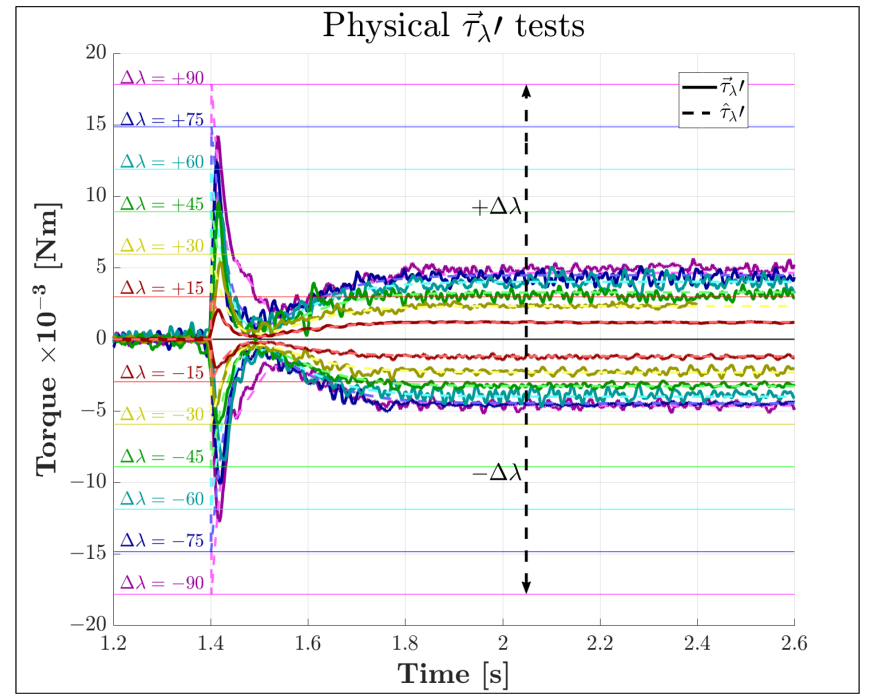
\includegraphics[width=\textwidth]{graphs/tau-lambda}
\caption{Physical induced $\vec{\tau}_\lambda\hspace{-1pt}'$ torque}
\label{fig:tau-lambda}
\end{subfigure}
\begin{subfigure}{0.495\textwidth}
\centering
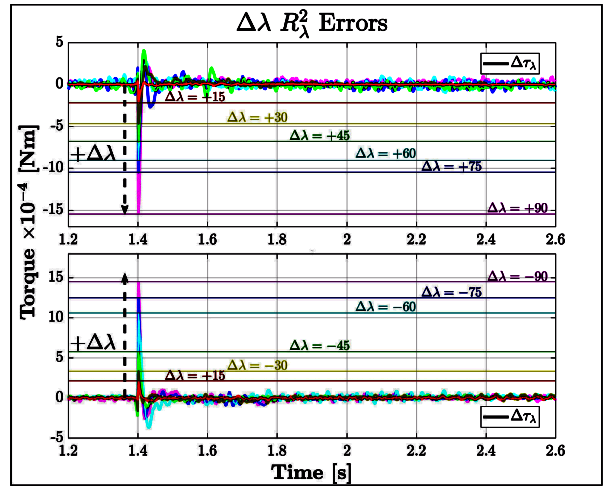
\includegraphics[width=\textwidth]{graphs/tau-lambda-r}
\caption{$\sqrt{R^2_{\lambda}}$ errors for $\vec{\tau}_\lambda\hspace{-1pt}'$}
\label{fig:tau-lambda-r}
\end{subfigure}
\vspace{-4pt}
\caption{Inner ring test rig response}
\label{fig:inner-ring-response-test}
\vspace{-10pt}
\end{figure}
\par
The error between the physically measured $\vec{\tau}_\lambda\hspace{-1pt}'(\lambda_i)$ and modelled $\hat{\tau}_\lambda\hspace{-1pt}'(\lambda_i)$ torques are shown in Fig:\ref{fig:tau-lambda-r}. Peak induced torque as a result of a commanded rotation $\Delta\lambda_i$ increases proportionally with that step size. The co-axial support bearings on the test rig, despite being de-greased and cleaned ultrasonically, still dampened the faster elements of the transient torque response; moreover the overall small magnitude of measured signals meant samples were susceptible to vibration noise transformed through the mechanical structure. There is, however, a clear correlation between the simulated and physically measured signal. Within a margin of error, and considering the tolerances of the test rig, such step changes corroborate the proposed inner ring model in Eq:\ref{eq:model-inner}.
\par
Verification of the dynamics for the middle ring response requires more in-depth discussion. Unlike the inner ring's response, described in Eq:\ref{eq:model-inner}; the middle ring's torque $\vec{\tau}_\alpha(\lambda_i,\alpha_i)$ from Eq:\ref{eq:torque-induced-middle} is \emph{\textbf{not equivalent}} to the generalized torque response acting on the middle ring system $\vec{\mathbf{V}}(\lambda_i,\alpha_i)$, Eq:\ref{eq:3.86g}. As mentioned previously $\vec{\mathbf{V}}(\lambda_i,\alpha_i)$ includes a transformed component of the inner ring's generalized response $R_y(\alpha_i)\vec{\mathbf{U}}(\lambda_i)$ from Eq:\ref{eq:generalized-inner}, whilst the \emph{servo response torque} $\vec{\tau}_\alpha(\lambda_i,\alpha_i)$ \emph{\textbf{does not}}. 
\par
To differentiate the servo's response torque $\vec{\tau}_\alpha(\lambda_i,\alpha_i)$ and the physical (generalized) torque being considered and tested here, $\vec{\Gamma}_\alpha(\lambda_i,\alpha_i)$ is used to refer to the induced torque response from the middle ring assembly's net rotation. 
\par
That torque is the measured component of the middle ring response and equivalent to the generalized torque response. Reiterating the equation for the expected generalized torque $\vec{\mathbf{V}}(\lambda_i,\alpha_i)$ from Eq:\ref{eq:3.86g}, now with included gravitational and aerodynamic torque components and induced torques as a result of the inner ring's rotation:
\begin{multline} \label{eq:model-middle}
\vec{\Gamma}_\alpha(\lambda_i,\alpha_i)=R_y(\alpha_i)\vec{\mathbf{U}}(\lambda_i)+\big(\dot{J}_p'\big)\dot{\vec{\alpha}}_i+\Big(\dot{J}_n''-R_y(\alpha_i)\big(\dot{J}_n'\big)R_y^{-1}(\alpha_i)\Big)\dot{\vec{\lambda}}_i'+\Big(\dot{J}_r''-R_y(\alpha_i)\big(\dot{J}_r'\big)R_y^{-1}(\alpha_i)\Big)\vec{\Omega}_i''
\\
+\big(J_\text{p}'\big)\ddot{\vec{\alpha}}_i+\dot{\vec{\alpha}}_i\times \Big(\big(J_p'\big)\dot{\vec{\alpha}}_i+\big(J_n''\big)\dot{\vec{\lambda}}_i\hspace{-2pt}'+\big(J_r''\big)\vec{\Omega}_i\hspace{-2pt}''\Big)+R_y(\alpha_i)R_x(\lambda_i)\big(H(\Omega_i)\cdot\hat{Z}_{M_i}\big)+m_\text{p}\vec{C}_{\text{p}}\text{}\hspace{-2pt}''(\alpha_i,\lambda_i)\times\vec{G}_{M_i''}
\\
=\vec{\mathbf{V}}(\lambda_i,\alpha_i)~~~~\in\mathcal{F}^{M_i''}
\end{multline}
Where the term $\vec{C}_{\text{p}}\text{}\hspace{-2pt}''(\alpha_i,\lambda_i)$ is the net rotated center of gravity for the entire motor module as a function of both servo positions:
\begin{equation}
\vec{C}_\text{p}\text{}\hspace{-2pt}''(\alpha_i,\lambda_i)=\frac{m_\text{n}R_y(\alpha_i)R_x(\lambda_i)\vec{C}_\text{n}+m_\text{m}R_y(\alpha_i)\vec{C}_\text{m}}{m_\text{m}+m_\text{n}}
\end{equation}
With $m_\text{m}$ and $m_\text{n}$ being inner and middle ring structure's respective masses, $m_\text{m}=98~[\text{g}]$ and $m_\text{n}=92~[\text{g}]$ from Sec:\ref{sec:proto.inertia}.
Fig:\ref{fig:torque-middle} shows the test rig used to measure torque responses for the motor module assembly which containing both inner and middle ring assemblies. The inner ring servo $\lambda_i$ was tested both at a constant $\lambda_i=0$ and at intervals for steps of equivalent in inner and middle ring servo angles.
\par
\begin{figure}[htbp]
\centering
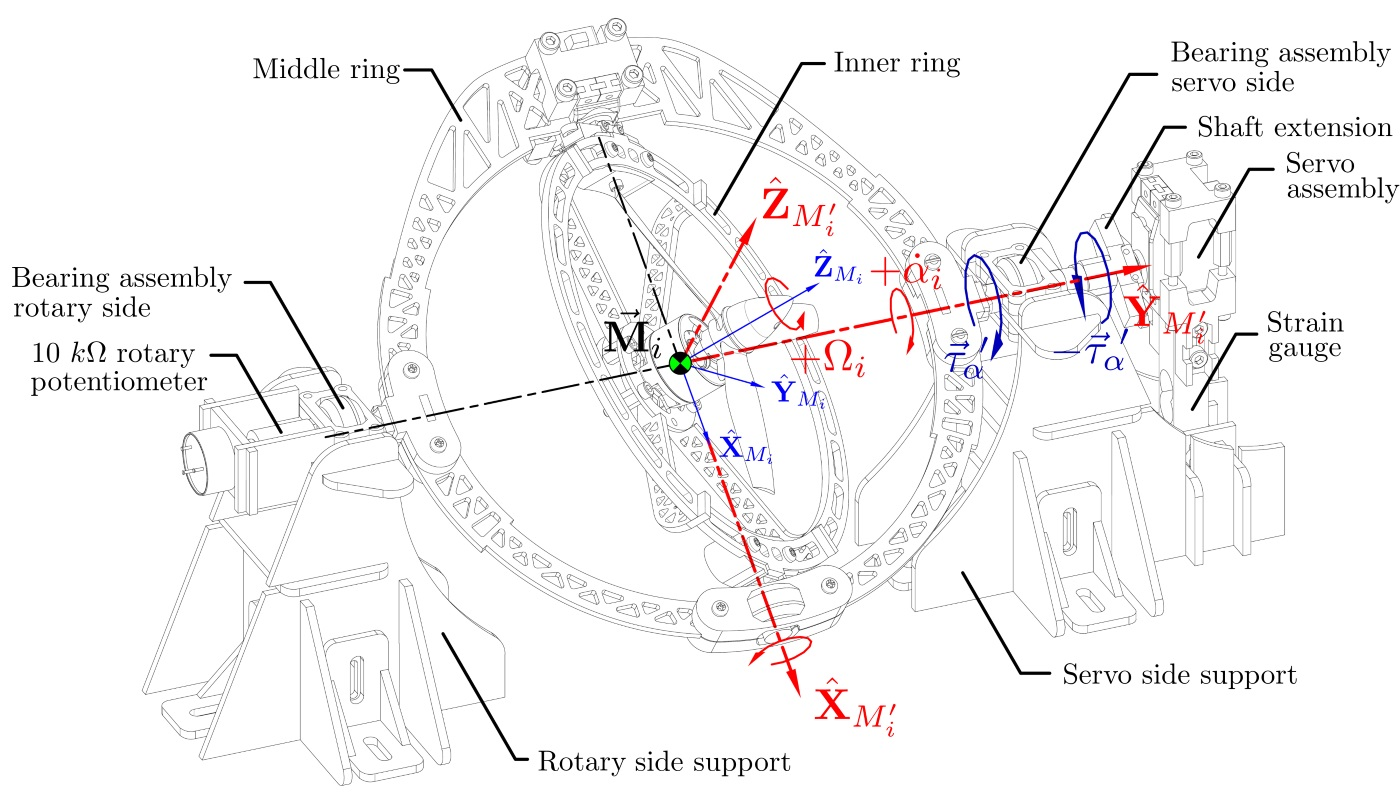
\includegraphics[width=\textwidth]{figs/torque-middle}
\vspace{-10pt}
\caption{Middle ring torque test rig}
\label{fig:torque-middle}
\vspace{-6pt}
\end{figure}
\par
The middle ring servo $\alpha_i$ applies an accelerating torque $\vec{\Gamma}_\alpha(\lambda_i,\alpha_i)$ to the assembly; the test rig isolates only the $\hat{Y}_{M_i''}$ component of that torque. Because the strain gauge encounters only that axial deflection, it then deflects proportionally to the physical torque :
\begin{equation}
\vec{\Gamma}_\alpha\text{}\hspace{-2pt}'(\lambda_i,\alpha_i)=\vec{\Gamma}_\alpha(\lambda_i\alpha_i)\cdot\hat{Y}_{M_i''}~~~~\in\mathcal{F}^{M_i''}
\end{equation}
Furthermore, the inner servo's torque contribution to Eq:\ref{eq:model-middle}, or $R_y(\alpha_i)\vec{\mathbf{U}}(\lambda_i)$, is small for any case where the propeller's rotational speed and the inner ring's servo speed are both roughly constant; $\dot{\Omega}_i\approx 0$ and $\dot{\lambda}_i\approx 0$. Fig:\ref{fig:tau-alpha} plots results for measured torque $\vec{\Gamma}_\alpha\text{}\hspace{-2pt}'(\lambda_i,\alpha_i)$ and expected torque estimate $\hat{\Gamma}_\alpha\text{}\hspace{-2pt}'(\lambda_i,\alpha_i)$ for a constant inner ring servo position $\lambda_i=0$. Again the propeller's rotational speed was kept constant at $\Omega_i=+6000~\text{RPM}$. 
\par
The error deviation between the two measured and estimated torques is shown in Fig:\ref{fig:tau-alpha-r}, with larger fast torque spikes leading to damped errors of greater magnitude. Steps performed in Fig:\ref{fig:middle-response-test} at intervals $\Delta\alpha_i=\pm[1/12\pi,~2/12\pi~\ldots~5/12\pi,~6/12\pi]$ simply verify the middle ring's inertial contribution to the model. With no inner ring servo velocity; $\dot\lambda\not=0$, the complex dynamics are not completely present. It is however worth noting the dis-symmetry in the shape of the torque's positive and negative responses resulting from unsymmetrical inertias in $J_p$ from Eq:\ref{eq:inertia.middle.b}.
\begin{figure}[htbp]
\centering
\begin{subfigure}{0.49\textwidth}
\centering
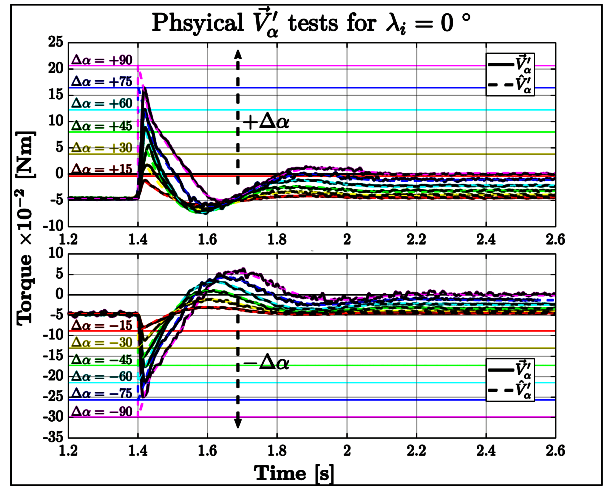
\includegraphics[width=\textwidth]{graphs/tau-alpha}
\caption{Test rig results for $\hat{\Gamma}_\alpha$}
\label{fig:tau-alpha}
\end{subfigure}
\begin{subfigure}{0.49\textwidth}
\centering
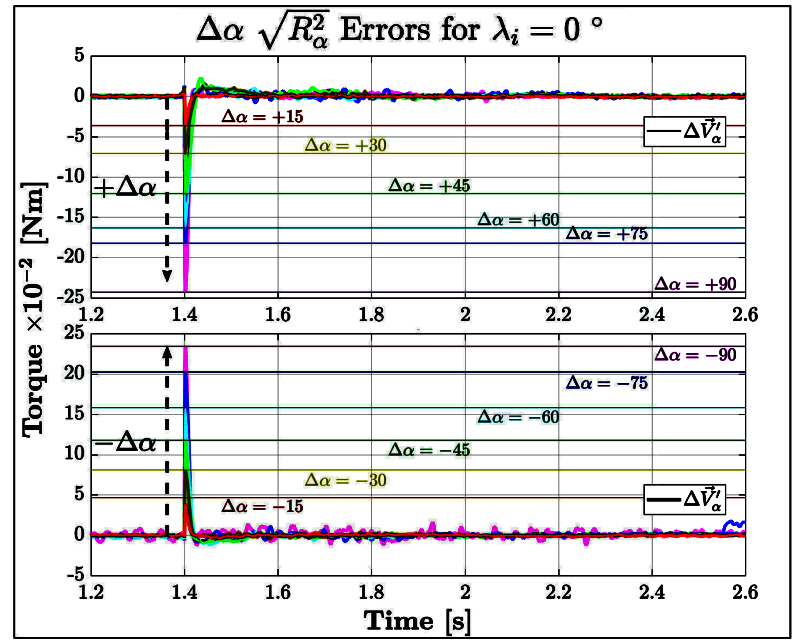
\includegraphics[width=\textwidth]{graphs/tau-alpha-r}
\caption{Errors for $\sqrt{R^2_{\alpha}}$}
\label{fig:tau-alpha-r}
\end{subfigure}
\vspace{-8pt}
\caption{Middle ring response}
\label{fig:middle-response-test}
\vspace{-16pt}
\end{figure}
\par
The larger inertia being rotated by the $\alpha_i$ middle ring servo contributes towards a greater initial torque spike as a result of the angular acceleration from $\ddot{\alpha_i}$, in the order of $\times 10^{-1}~\text{Nm}$. The damping effect applied by the support bearing is more pronounced in the middle ring case, producing errors with greater magnitudes in Fig:\ref{fig:tau-alpha-r}. Without introducing a step for the inner ring $\lambda_i$, the response in Fig:\ref{fig:middle-response-test} is mostly a scaled version of the inner ring response in Fig:\ref{fig:inner-ring-response-test}.
\par
Finally, testing combined rotations of $\lambda_i$ and $\alpha_i$ stepped together, Fig:\ref{fig:tau-alpha-lam-response-test} shows the manifestation of the complex dynamics involved in a single motor module's combined actuator action. Each interval step is performed with equal servo step sizes; $\Delta\lambda_i=\Delta\alpha_i$ for $\lambda_i,\alpha_i\in\pm[1/12\pi,~2/12\pi~\ldots~5/12\pi,~6/12\pi]$. Still using a constant propeller speed $\Omega_i=+6000~\text{rpm}$, the introduction of gyroscopic torque begins to affect the step response shown in Fig:\ref{fig:tau-alpha-lam}. As $\lambda_i$ and $\alpha_i$ approach $\pi/2$ rad, the propeller's rotational aerodynamic torque begins to make a contribution towards Eq:\ref{eq:model-middle} as its rotational axis aligns with the measurement axis $\hat{Y}_{M_i''}$.
\begin{figure}[htbp]
\centering
\begin{subfigure}{0.49\textwidth}
\centering
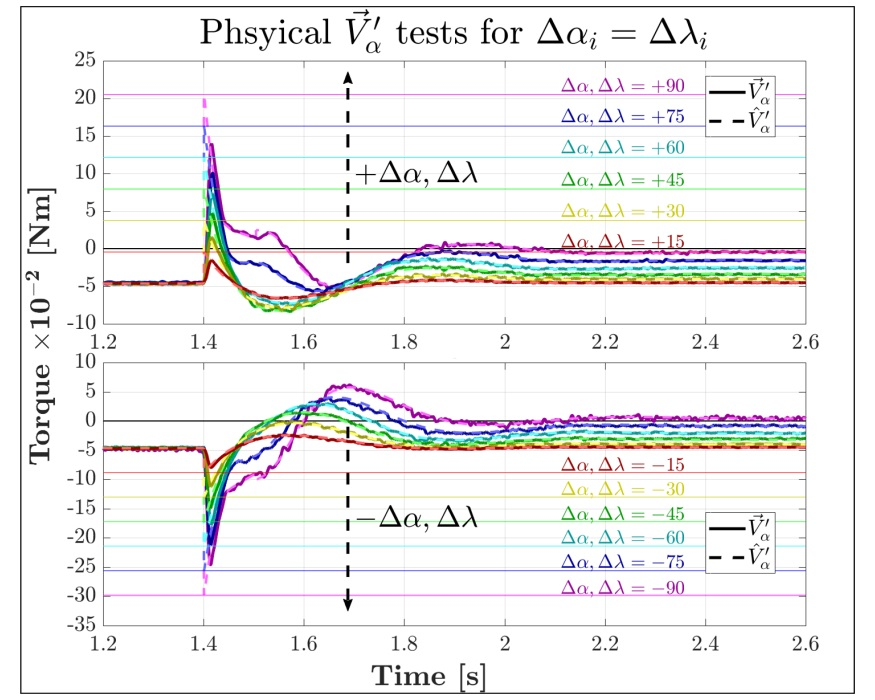
\includegraphics[width=\textwidth]{graphs/tau-alph-lam}
\caption{Test rig results for $\hat{\Gamma}_\alpha$ with $\Delta\alpha=\Delta\lambda$}
\label{fig:tau-alpha-lam}
\end{subfigure}
\begin{subfigure}{0.49\textwidth}
\centering
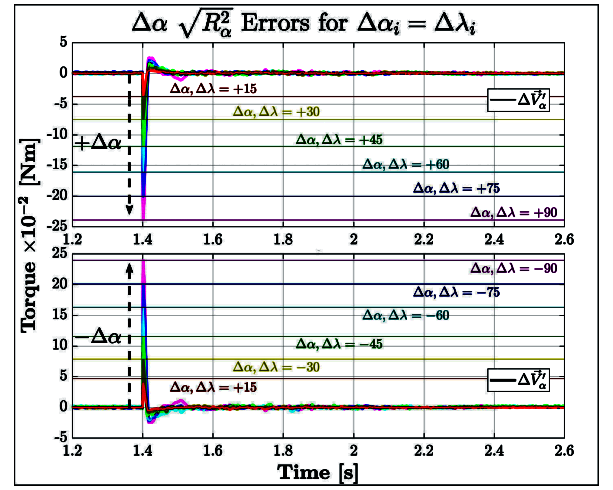
\includegraphics[width=\textwidth]{graphs/tau-alph-lam-r}
\caption{Errors for $\sqrt{R^2_{\alpha}}$}
\label{fig:tau-alpha-lam-r}
\end{subfigure}
\vspace{-8pt}
\caption{Combined middle ring response}
\label{fig:tau-alpha-lam-response-test}
\vspace{-16pt}
\end{figure}
\par
The unsymmetrical inertia of a motor module, even at rest and due to the unbalanced servo weight in Fig:\ref{fig:inertia-middle}, skews the response torque; shown in previous tests in Fig:\ref{fig:tau-alpha}. Combining both servos to be actuated at the same time further skews the torque response curve. The induced gyroscopic product of both rotations constructively and destructively affects Eq:\ref{eq:model-middle} depending on the rotational sense. Only positive $\Delta\alpha_i=\Delta\lambda_i$ tests were performed, conversely $\Delta\alpha_i=-\Delta\lambda_i$ would have a reciprocal effect. Again the fast initial torque spike is damped by the test set-up bearings; resulting in an initial error plotted in Fig:\ref{fig:tau-alpha-lam-r}, which subsequently reduces very quickly. Because the inner ring has a center of gravity, $\vec{C}_\text{n}$ in Eq:\ref{eq:body-net-inner.b}, very close to the module's center of rotation, steady state torque offsets from gravitational torque contributions to $\vec{\Gamma}_\alpha\hspace{-2pt}'(\lambda_i,\alpha_i)$ are almost independent of the inner ring $\lambda_i$ servo position. 
\par
\emph{\color{Gray} Each of the above step tests in Fig:\ref{fig:inner-ring-response-test},Fig:\ref{fig:middle-response-test} and Fig:\ref{fig:tau-alpha-lam-response-test} were each performed three times and the resultant measured torques were averaged over those three tests. What is plotted are the ten sample moving averages of those combined data sets from the three independent tests for each angular step.}
\par
\emph{\color{Gray}The above responses are pertinent to simulation and plant dependent feedback compensation. The simulation environment is structured such that the torques are produced as responses from Newtonian movement at every step interval. In due course it would be more efficient (and less stiff) for the simulation to exploit an implicit Euler\cite{physicallybased,multibodydynamics} coordinate system in lieu of the cartesian response equations developed above. However this was not implemented in Ch:\ref{ch:simulation} and remains open to further testing and simulation\ldots}
\subsubsection{Body Response Simulation Tests}
\label{subsubsec:dynamicsimulation}
To corroborate and test the presented dynamic model for the vehicle's net motion, described in Eq:\ref{eq:3.109}, a series of experimental simulations are performed using the proposed differential equations of motion and the subsequent results are discussed. The simulation environment used here is a simplified, open loop version of the one presented later in Sec:\ref{sec:simulation.block}. In some cases the plant inputs are reduced to net forces and torques, in other cases explicit propeller speeds and servo rotational positions are commanded as inputs. Considering the mass properties of the quadrotor design in Sec:\ref{sec:proto.design}, force and torque inputs for a stable hover to be actuated by the control plant are as follows:
\begin{equation}\label{eq:basic-hover}
\vec{\nu}_h=\begin{bmatrix}
\vec{F}_h\\
\vec{\tau}_h
\end{bmatrix}=m_b\begin{bmatrix}
\vec{G}_b\\
\vec{C}_b(u)\times \vec{G}_b
\end{bmatrix}=\begin{bmatrix}
\begin{bmatrix}
0 & 0 & 15.45
\end{bmatrix}^T
\\
\begin{bmatrix}
0.25 & 0.50 & -0.08
\end{bmatrix}^T
\end{bmatrix}
~~~~\begin{bmatrix}
[\text{N}]\\
[\text{N.mm}]
\end{bmatrix}
\end{equation}
where the force input $\vec{F}_h$ acts to oppose the gravitational acceleration acting on the body and the torque $\vec{\tau}_h$ opposes the gravitational torque arm produced by the body's eccentric center of gravity. Note that Eq:\ref{eq:basic-hover} does not include terms associated with rotational aerodynamic torque $\vec{H}(\Omega_i,\lambda_i,\alpha_i)$ from \ref{sec:dynamics.aero}, such terms require feedback compensation in closed loop. Simulating hover conditions will not provide any useful insight, but the commanded plant inputs for a hovering state do provide a suitable starting values to which input offsets can be applied. 
\begin{figure}[hbtp]
\vspace{-12pt}
\centering
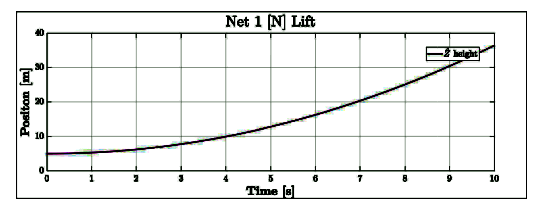
\includegraphics[width=0.8\textwidth]{graphs/upward_acceleration}
\vspace{-10pt}
\caption{Upward lift test}
\label{fig:upward_accl}
\end{figure}
\par
Adding an extra $1~[\text{N}]$ of lift should result in $\approx 0.6~[\text{m.s}^{-2}]$ of upward acceleration being applied to the body. Fig:\ref{fig:upward_accl} shows the simulation's position response to that added lift force where height is the only affected state variable. Starting from a height of $5~[\text{m}]$, the simulated vehicle rises to around $36.5~[\text{m}]$ after a time of $10~[\text{s}]$, as expected. A simple upward thrust test confirms the effect gravity and linear acceleration has on the model.
\par
Testing differential torque inputs and subsequent attitude responses, a small ($1\%$) difference between the rotational speed's of propellers 1 and 3 is applied. The differential speeds are offset from hovering conditions which command $\Omega_{1,3}=+10540~[\text{RPM}]$ and $\Omega_{2,4}=-10540~[\text{RPM}]$. If the first motor module's propeller speed is reduced and the third motor module's propeller speed is increased then the net torque applied is a positive pitching torque about the body's $\hat{Y}_b$ axis, forcing the vehicle's pitch attitude $\theta$ to increase. The applied speed offset is $\pm 53~[\text{RPM}]$ which produces an approximate differential torque $+0.3\cdot\hat{\j}~[\text{N.mm}]$ about the body frame's origin $\vec{\mathbf{O}}_b$. 
\begin{figure}[htbp]
\vspace{-8pt}
\centering
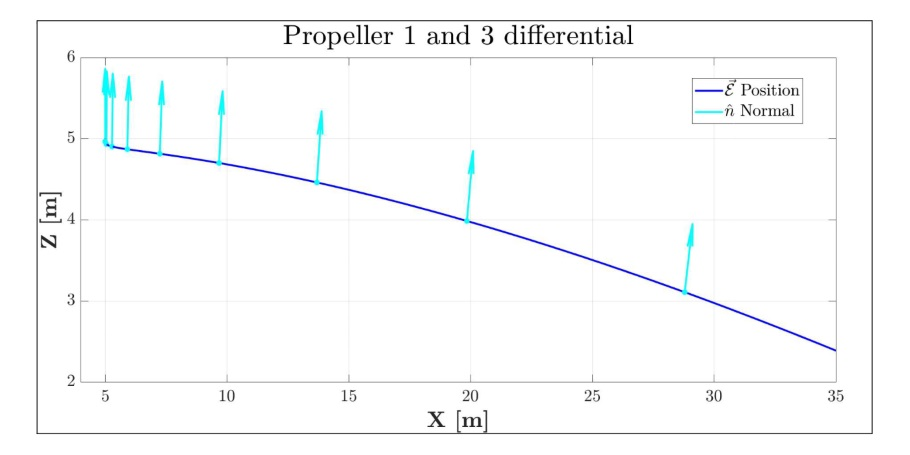
\includegraphics[width=0.75\textwidth]{graphs/propeller_differential}
\vspace{-6pt}
\caption{Differential torque input}
\label{fig:differential_prop}
\vspace{-10pt}
\end{figure}
\par
Fig:\ref{fig:differential_prop} shows the XZ plot of the vehicle's position following the differential propeller/torque input. The simulation starts at position $\vec{\mathcal{E}}_0=[5~5~5]^T~[\text{m}]$. Over the course of a $10~[\text{s}]$ simulation, the applied torque slowly pitches the body's normal away from its origin whilst the $\hat{X}$ axis displacement increases. Each normal vector is plotted at a regular time interval of $1~[\text{s}]$. 
\par
Then applying module servo rotations to the first and third motor modules. Using $\lambda_{1,3}=1\text{\textdegree}$ to redirect the produced thrust vectors away from their stable hovering positions, this rotation applies an effective yaw moment about the $\hat{Z}_b$ axis. The redirection of the two thrust vectors away from their stable hovering positions without increasing their magnitudes (propeller speeds) will adversely affect the hovering altitude's. The net lift force will be reduced by the thrust vector redirection, reducing the net lift force to $\approx 15.4~[\text{N}]$ and applying an $\approx-26.3\cdot\hat{k}~[\text{N.mm}]$ yaw torque.
\begin{figure}[hbtp]
\vspace{-8pt}
\centering
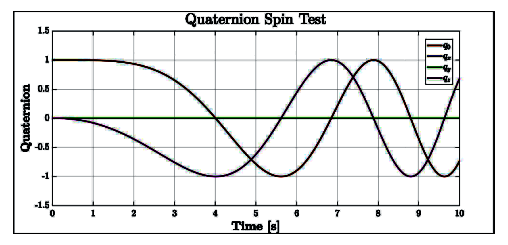
\includegraphics[width=0.8\textwidth]{graphs/spin_quaternion}
\vspace{-6pt}
\caption{Quaternion from yaw torque}
\vspace{-10pt}
\label{fig:spin}
\end{figure}
\par
The differential torque about the $\hat{Z}_b$ axis only affects the attitude's yaw angle $\psi$, pitch $\phi$ and roll $\theta$ remain unchanged. Fig:\ref{fig:spin} shows how that yaw torque, created by redirecting motor module's thrust vectors, produces an oscillatory motion in the attitude plant. The reduced lift force from redirection of the two motor module thrust vectors causes the vehicle to slowly descend from its hovering height of $5~[\text{m}]$, shown in Fig:\ref{fig:spin_position}. This particular test shows that minor perturbations away from a stable hover point causes large deviations in state variables, especially in the attitude plant. Leading to the conclusion that open loop hovering stability is extremely fragile and necessitates the need for closed loop position control to achieve the desired goal of attitude and position setpoint tracking.
\begin{figure}[htbp]
\centering
\vspace{-8pt}
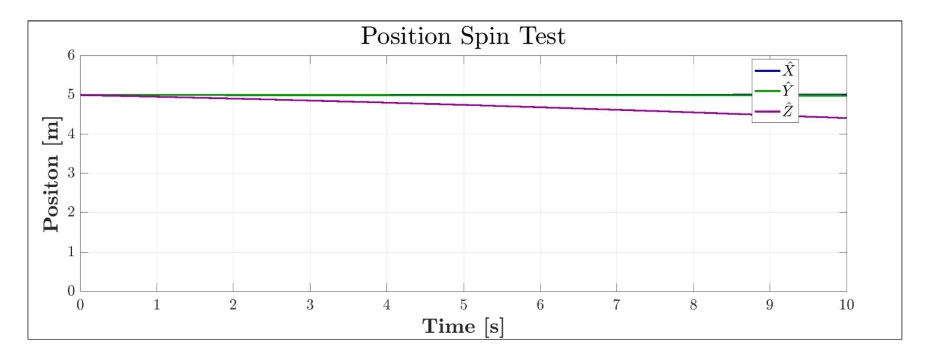
\includegraphics[width=0.8\textwidth]{graphs/spin_position}
\vspace{-6pt}
\caption{Position descent from yaw spin}
\vspace{-10pt}
\label{fig:spin_position}
\end{figure}
\par
Whilst none of the above simulated results are entirely unexpected, especially considering all the dynamics are derived from established fundamental theorems, the simulations and physical tests performed provide some degree of certainty to proposed model for the multibody system. The only way to truly ascertain the absolute accuracy of the equations of motion is to compare them to physical flight test data which is, unfortunately, beyond the scope of this investigation.
%====================================================
\section{Consolidated Model}
\label{sec:dynamics.model}
%====================================================
Reiterating the different responses detailed above and consolidating the state equations from Eq:\ref{eq:states.a}-\ref{eq:states.d}. Then lifting the attitude states to $\mathbb{Q}\in\mathbb{R}^4$ using quaternions. Also introducing the nonlinear inertial and gyroscopic responses to induced perturbations, $\vec{\tau}_\lambda(\lambda_i)$ and $\vec{\tau}_\alpha(\lambda_i,\alpha_i)$ from Eq:\ref{eq:torque-induced-inner} and Eq:\ref{eq:torque-induced-middle} respectively, with nonlinear inertial matrix terms $J_b(\vec{u})$ from Sec:\ref{sec:proto.inertia}. Net forces and torques $\vec{F}_{\mu}(\vec{u})$ and $\vec{\tau}_{\mu}(\vec{u})$ are controllable inputs to be designed by a higher level setpoint tracking controller discussed next in Ch:\ref{ch:control}. The exact actuator effectiveness and allocation schemes are explored thereafter in Ch:\ref{ch:allocation}. The vehicle's \emph{inertial frame} position and \emph{body frame} velocity differential equations are:
\begin{subequations}\label{eq:quaternion-states}
\begin{equation}\label{eq:quaternion-states-velocity}
\dot{\vec{\mathcal{E}}}_I=Q_b^*\otimes\vec{v}_b\otimes Q_b~~~~\in\mathcal{F}^I
\end{equation}
\vspace{-12pt}
\begin{equation}\label{eq:quaternion-states-acceleration}
\dot{\vec{v}}_b=m_b^{-1}\big(-\vec{\omega}_b\times m_b\vec{v}_b+Q_b\otimes m_b\vec{G}_I\otimes Q_b^*+\vec{F}_\mu(\hat{u})\big)~~~~\in\mathcal{F}^b
\end{equation}
Similarly the vehicle's attitude quaternion rate and angular acceleration are respectively:
\begin{equation}\label{eq:quaternion-states-quaternion}
\dot{Q}_b=\frac{1}{2}Q_b\otimes \vec{\omega}_b ~~~~\in\mathcal{F}^I
\end{equation}
\vspace{-10pt}
\begin{equation}\label{eq:quaternion-states-angular}
\dot{\vec{\omega}}_b=J_b(\hat{u})^{-1}\big(-\vec{\omega}_b \times J_b(\hat{u})\vec{\omega}_b-\vec{\tau}_b(\hat{u})+\vec{\tau}_g+\vec{\tau}_H+\vec{\tau}_{\mu}(\hat{u})\big)~~~~\in\mathcal{F}^b
\end{equation}
The actuator space $\vec{u}$ is defined as per Eq:\ref{eq:actuator-space}, where each actuator has its own transfer function $C(s)$ described in Sec:\ref{subsec:proto.design.transfer}, leading to an actuator state estimate $\hat{u}$ used for control inputs $\vec{F}_\mu(\hat{u})$ and $\vec{\tau}_{\mu}(\hat{u})$ and feedback compensation terms.
\begin{equation}
\vec{u}\triangleq\big[\Omega_1^+,~\lambda_1,~\alpha_1,~\ldots~\Omega_4^-,~\lambda_4,~\alpha_4 \big]~~~~\in\mathbb{U}\in\mathbb{R}^{12}
\end{equation}
\end{subequations}
Control force and torque plant inputs, $\vec{F}_\mu(\hat{u})$ and $\vec{\tau}_\mu(\hat{u})$ respectively, are a combination of Eq:\ref{eq:generalized-net-forces} with three dimensional thrust vectors $\vec{T}(\Omega_i)$ as per the quaternion analogue of Eq:\ref{eq:motor-module-force-redirect}. Both are later abstracted to virtual control inputs later in the control allocation design Ch:\ref{ch:allocation}.
\begin{subequations}\label{eq:quaternion-inputs}
\begin{equation}
\vec{F}_\mu(\hat{u})=\sum_{i=1}^4 \vec{T}(\Omega_i,\lambda_i,\alpha_i)=\sum_{i=1}^4 Q_{M_i}^*\otimes T(\Omega_i)\otimes Q_{M_i}~~~~\in\mathcal{F}^b
\end{equation}
\vspace{-6pt}
\begin{equation}
\vec{\tau}_\mu(\hat{u})=\sum_{i=1}^4 \vec{L}_i\times\vec{T}(\Omega_i,\lambda_i,\alpha_i)=\sum_{i=1}^4 \vec{L}_i\times\big(Q_{M_i}^*\otimes T(\Omega_i)\otimes Q_{M_i}\big)~~~~\in\mathcal{F}^b
\end{equation}
\end{subequations}
The torque term $\vec{\tau}_H$ is the net aerodynamic torque produced by the propeller's rotational velocity, to be compensated for in \emph{\textbf{feedback}}, and as such is separated from the controllable inputs in Eq:\ref{eq:quaternion-inputs}:
\begin{equation}\label{eq:consolidated-h-torque}
\vec{\tau}_H=\sum_{i=1}^4 \vec{H}(\Omega_i,\lambda_i,\alpha_i)=\sum_{i=1}^4 Q_{M_i}^*\otimes \vec{H}(\Omega_i)\otimes Q_{M_i}~~~~\in\mathcal{F}^b
\end{equation}
Scalar thrust $T(\Omega_i)$ is a function of the propeller's rotational velocity whereas $\vec{T}(\Omega_i,\lambda_i,\alpha_i)$ is that thrust's three dimensional counterpart in $\mathcal{F}^b$. Equivalently $H(\Omega_i)$ is the scalar aerodynamic torque in $\mathcal{F}^{M_i}$ about each motor's rotor $\hat{Z}_{M_i}$-axis, whereas $\vec{H}(\Omega_i,\lambda_i,\alpha_i)$ is the torque vector counterpart in $\mathcal{F}^b$. Both thrust and aerodynamic torque terms are calculated from their respective coefficients (plotted in Fig:\ref{fig:coeffs-plot}):
\begin{subequations}\label{eq:dynamic-plant-inputs}
\begin{equation}\label{eq:aerodynamic-thrust}
\vec{T}(\Omega_i)= C_T(J)\rho\Omega_i^2D^4\cdot\hat{Z}_{M_i}~~~~\in\mathcal{F}^{M_i}
\end{equation}
\vspace{-10pt}
\begin{equation}\label{eq:aerodynamic-torque}
\vec{H}(\Omega_i)= C_P(J)\rho\Omega_i^3D^5 \big(1/R\Omega_i\big)\cdot\hat{Z}_{M_i}~~~~\in\mathcal{F}^{M_i}
\end{equation}
\end{subequations}
Recalling that $\Omega_i$ for aerodynamic calculations in Eq:\ref{eq:aerodynamic-thrust} and Eq:\ref{eq:aerodynamic-torque} has units $[\text{RPS}]$. The nonlinear torque responses from multibody configuration changes in Eq:\ref{eq:net-body-response} are introduced as terms for  feedback compensation, calculated from instantaneous actuator estimates:
\begin{equation}\label{eq:actuator-torque}
\vec{\tau}_b(\hat{u})\triangleq\dot{J}_b(\hat{u})\vec{\omega}_b+\sum_{i=1}^{4}\Big[\vec{\tau}_\alpha\hspace{-1pt}'(\lambda_i,\alpha_i)+\vec{\tau}_\lambda\hspace{-2pt}''(\lambda_i)+\vec{\omega}_b\times\Big(\big(J_p''\big)\dot{\vec{\alpha}}_i'+\big(J_n'''\big)\dot{\vec{\lambda}}_i''+\big(J_r'''\big)\vec{\Omega}_i'''\Big)\Big]~~~~\in\mathcal{F}^b
\end{equation}
with $\vec{\tau}_\alpha\hspace{-2pt}'(\lambda_i,\alpha_i)$ and $\vec{\tau}_\lambda\hspace{-2pt}''(\lambda_i)$ both transformed to the body frame $\mathcal{F}^b$. Then including variable gravitational torque as a result of an eccentric center of gravity from Eq:\ref{eq:mass-center.b}; also dependent on the vehicles configuration:
\begin{equation}\label{eq:consolidated-grav-torque}
\vec{\tau}_g=\Delta \vec{C}_\text{G} \times\vec{G}_b=\big(\vec{\mathbf{O}}_b-\vec{C}_\text{b}(u)\big)\times\vec{G}_b~~~~\in\mathcal{F}^b
\end{equation}
And finally the vehicles net rotational inertia, aligned and centered with the body frame. That inertia is calculated as a function of all actuator positions; taken from Eq:\ref{eq:body-net-2} and given as:
\begin{equation}
\underset{\vec{\mathbf{O}}_b}{J_b(\hat{u})}=\underset{\vec{\mathbf{O}}_b}{J'_\text{y}}+\sum_{i=1}^{4} \underset{\vec{\mathbf{O}}_b}{J_\text{n}(\hat{u}_i)}+\sum_{i=1}^{4} \underset{\vec{\mathbf{O}}_b}{J_\text{m}(\hat{u}_i)}~~~~u\in\mathbb{U}
\end{equation}
where $\vec{u}_i$ is the $\text{i}^{th}$ motor module's actuator position: $\vec{u}_i\triangleq [\Omega_i~\lambda_i~\alpha_i]^T$ and $\hat{u}_i$ is the position estimate subject to those actuator's transfer functions. Both attitude (either euler angles $\vec{\eta}$ or quaternions $Q_b$) and translational position states $\vec{\mathcal{E}_I}$ could indeed be combined into a single state $\vec{\mathbf{x}}_b$. That could then be used for a complete state feedback control law which could potentially exploit or linearize the cross-coupling between the angular and translational plants. Such an approach would, however, dramatically increase the complexity in tuning actual control parameters (see Sec:\ref{sec:simulation.tuning}). Controllers for attitude and position loops are designed and optimized independently.